\documentclass[11pt]{article}
\usepackage[T1]{fontenc}
\usepackage{lmodern}
\usepackage[margin=1.05in]{geometry}
\usepackage{amsmath,amssymb,amsthm,mathtools}
\usepackage{microtype}
\usepackage{enumitem}
\usepackage{tikz}
\usetikzlibrary{arrows.meta,positioning}
\usepackage[colorlinks=true,linkcolor=blue!45!black,citecolor=blue!45!black,urlcolor=blue!45!black]{hyperref}
\hypersetup{pdftitle={Riesz transforms and uniform rectifiability in higher codimension},pdfauthor={OpenAI},pdfsubject={Riesz transforms, Ahlfors--David regularity, and quantitative rectifiability}}
\newcommand{\R}{\mathbb R}
\renewcommand{\H}{\mathcal H}
\DeclareMathOperator{\supp}{supp}
\DeclareMathOperator{\Lip}{Lip}
\DeclareMathOperator{\dist}{dist}
\DeclareMathOperator{\diam}{diam}
\DeclareMathOperator{\spt}{spt}
\newtheorem{theorem}{Theorem}[section]
\newtheorem{proposition}[theorem]{Proposition}
\newtheorem{lemma}[theorem]{Lemma}
\newtheorem{corollary}[theorem]{Corollary}
\theoremstyle{definition}
\newtheorem{definition}[theorem]{Definition}
\theoremstyle{remark}
\newtheorem{remark}[theorem]{Remark}
\numberwithin{equation}{section}
\setcounter{tocdepth}{2}
\setlist{topsep=4pt,itemsep=2pt,parsep=0pt}
\title{Riesz transforms and uniform rectifiability\\in higher codimension}
\author{OpenAI}
\date{September 24, 2026}
\begin{document}
\maketitle
\begin{abstract}
We prove that an $n$-Ahlfors--David regular Radon measure on $\R^d$
is uniformly $n$-rectifiable if its $n$-dimensional Riesz transform is
uniformly bounded from scalar $L^2(\mu)$ to vector-valued $L^2(\mu)$
over all positive hard truncations, for integers $d\ge4$ and
$2\le n\le d-2$.
This gives a positive answer to the David--Semmes Riesz-transform question
in its remaining higher-codimension range. The conclusion gives uniform
big pieces of Lipschitz images of Euclidean balls.
\end{abstract}
\tableofcontents
\section{The quantitative theorem and normalized pairings}
\label{sec:background}

Singular integral estimates can detect the geometry of a measure even
when its support has no initial parametrization. The Riesz transform is
a particularly natural test: its kernel records the direction between
two points as well as their separation. We prove that, for an
integer-dimensional Ahlfors--David regular measure in the intermediate
codimensions, its $L^2$ boundedness forces a quantitatively rectifiable
support.

Throughout the paper, $d$ and $n$ are positive integers with $n\le d$,
and balls are open Euclidean balls. A Radon measure is
a Borel measure that is finite on compact sets and regular. For such a
measure $\mu$ on $\R^d$, write $E=\supp\mu$ and $D_E=\diam E$, allowing
$D_E=\infty$. When $E$ is empty, set $D_E=0$.

\begin{definition}[Ahlfors--David regularity]\label{def:ad}
A Radon measure $\mu$ on $\R^d$ is \emph{$n$-Ahlfors--David regular}
with constant $C_{\rm AD}\ge1$ if
\[
 C_{\rm AD}^{-1}r^n\le\mu(B(x,r))\le C_{\rm AD}r^n
 \qquad(x\in E,\quad 0<r\le D_E).
\]
We call these positive radii \emph{admissible}. The inequalities have
no instances when $D_E=0$.
\end{definition}

For $z\ne0$ let $K_n(z)=z/|z|^{n+1}$. The hard truncations of the
$n$-dimensional Riesz transform are
\begin{equation}\label{eq:hard-truncation}
 R_{\mu,\varepsilon}f(x)
 =\int_{|x-y|>\varepsilon} K_n(x-y)f(y)\,d\mu(y),\qquad\varepsilon>0.
\end{equation}
We say that the transform is bounded on $L^2(\mu)$ with bound
$C_{\rm R}$ if, for every real scalar $f\in L^2(\mu)$ and every
$\varepsilon>0$, the integral in \eqref{eq:hard-truncation} defines an
$\R^d$-valued $L^2(\mu)$ function and
\begin{equation}\label{eq:riesz-bound}
 \|R_{\mu,\varepsilon}f\|_{L^2(\mu;\R^d)}
 \le C_{\rm R}\|f\|_{L^2(\mu)}.
\end{equation}
No pointwise principal-value hypothesis is imposed. For a nontrivial
regular support, the integrals in \eqref{eq:hard-truncation} are
absolutely convergent for every $x$ and every $f\in L^2(\mu)$;
this follows from Lemma~\ref{lem:global-growth} below.

\begin{definition}[Uniform rectifiability]\label{def:ur}
An $n$-Ahlfors--David regular measure $\mu$ on $\R^d$ is
\emph{uniformly $n$-rectifiable} if there are $\theta>0$ and $M<\infty$
such that, for every $x\in E$ and $0<r\le D_E$, there is an
$M$-Lipschitz map
\[
 g:B_{\R^n}(0,r)\longrightarrow\R^d,
 \qquad
 \mu\bigl(B(x,r)\cap g(B_{\R^n}(0,r))\bigr)\ge\theta r^n.
\]
The constants are chosen before $x$ and $r$.
\end{definition}

\begin{theorem}\label{thm:main}
Let $d\ge4$ and $2\le n\le d-2$ be integers. Let $\mu$ be an
$n$-Ahlfors--David regular Radon measure on $\R^d$ satisfying
\eqref{eq:riesz-bound}. Then $\mu$ is uniformly $n$-rectifiable in the
sense of Definition~\ref{def:ur}. Its constants $\theta$ and $M$ can
be chosen in terms of $d,n,C_{\rm AD}$ and $C_{\rm R}$ alone.
\end{theorem}

\subsection{History and the analytic question}

David and Semmes developed uniform rectifiability as a quantitative
form of rectifiability suited to singular integrals
\cite{DavidSemmes1991,DavidSemmes1993}. Among its equivalent
descriptions are big pieces of Lipschitz images and a packing condition
on balls where the support fails to approximate a plane from both
sides. Their question asks whether the boundedness of the Riesz
transform alone forces this geometry for an integer-dimensional
regular measure.

Mattila, Melnikov and Verdera established the planar implication using
the relation between the Cauchy integral, curvature and uniform
rectifiability \cite{MattilaMelnikovVerdera1996}. Curvature methods
also give the one-dimensional Riesz-transform implication in higher
ambient dimension; see \cite[Theorem~4]{Farag2000}.
Nazarov, Tolsa and Volberg proved the codimension-one implication
\cite{NazarovTolsaVolberg2014}.
They identify reliance on a maximum principle, for which they report
no known higher-codimension analogue, as the main obstacle to extending
their argument \cite[Section~1]{NazarovTolsaVolberg2014}.
Mas and Tolsa obtained a characterization in every integer dimension
$1\le n<d$ by an $L^2$ bound for the $\rho$-variation of the Riesz
truncations, with $\rho>2$ \cite[Theorem~1.3]{MasTolsa2014Variation}.
That hypothesis bounds the pointwise supremum, over decreasing positive
sequences $(\varepsilon_j)$, of
\[
 \left(\sum_j
   |R_{\mu,\varepsilon_{j+1}}f-R_{\mu,\varepsilon_j}f|^\rho
       \right)^{1/\rho}
\]
in $L^2(\mu)$. It controls changes across scales, rather than each
truncation separately. The present hypothesis is only the common bound
\eqref{eq:riesz-bound}; no variation estimate is assumed.
The remaining range for this bound-alone question,
$1<n<d-1$, is stated explicitly in \cite[Question~4.4]{Tolsa2026ICM}.
Theorem~\ref{thm:main} gives a positive answer in that range, with the
hard-truncation convention and the ball parametrizations stated
above.

Principal-value criteria address a different analytic hypothesis.
For a set of finite $\H^n$ measure, Tolsa characterized ordinary
rectifiability by almost-everywhere existence of Riesz principal values
\cite[Theorem~1.1]{Tolsa2008PrincipalValues}. That result neither assumes
only \eqref{eq:riesz-bound} nor asserts the quantitative ball-map
conclusion considered here.

Two parts of the quantitative-rectifiability literature are especially
relevant to the proof. The bilateral weak geometric lemma of David and
Semmes converts geometric packing into Lipschitz images; a precise
Euclidean formulation is recalled in
\cite[Theorem~2.5]{Tolsa2015Uniform}. Reflectionless-measure methods
organize compactness limits for which the Riesz transform has zero
oscillation against mean-zero tests; see
\cite{JayeNazarov2018I}. We prove the particular limiting and rigidity
statements needed here, including their tail normalizations.

Flat subballs and stability of flatness also form the geometric route
in Tolsa's theorem for uniform measures
\cite[Section~3]{Tolsa2015Uniform}. There the ball masses are exactly
proportional to $r^n$, and the stability step uses Preiss's rigidity at
infinity, recalled in \cite[Theorem~2.4]{Tolsa2015Uniform}.
Here AD regularity gives two-sided comparisons rather than exact ball
masses. The normalized-height energy and rigidity argument below
provides the required propagation without a uniform-measure rigidity
input.

Section~\ref{sec:consequences} applies the uniform-rectifiability
conclusion to obtain variation bounds and almost-everywhere principal
values for the Riesz transform and the odd $C^2$ kernels specified there.

\subsection{The main mechanism}

The analytic difficulty is to propagate geometric flatness to smaller
scales. We measure the error by the \emph{excess}, the scale-normalized
$L^2$ distance from an affine $n$-plane. Normal heights are the coordinates
of the displacement perpendicular to that plane. Weak convergence to a
plane makes the excess tend to zero; propagation requires an error small
relative to the initial excess. We therefore divide the normal heights
by that initial scale before passing to a limit.
This second limit is taken only when the Riesz pairings against compact
mean-zero Lipschitz tests are sufficiently small relative to the height
scale to vanish after normalization. Here the mean is taken against
the current measure, not against a presumed limiting plane.
The use of normal components to measure geometric deviation has a
related quantitative form on small-slope Lipschitz graphs in
\cite[Theorem~1.3]{Tolsa2008PrincipalValues}. Our compactness argument
instead works on moving AD-regular measures before any graph
parametrization has been established.

Testing the transform against an unnormalized normal height times a
cutoff produces a positive fractional energy. This estimate gives
compactness of the normalized heights through their second moments
and their integrals against Lipschitz tests. It also controls the
singular diagonal when passing to a limiting equation. The equation
holds against mean-zero tests and is therefore interpreted modulo
constants. Its order-one Fourier symbol, together with weighted
integrability at infinity, forces each limiting height to be affine. Approximation
by an affine graph now improves the original excess at the required
relative scale.

The remaining argument counts failures of this propagation on dyadic
cells of the support, nested pieces at successively halved scales.
The operator bound supplies descendants whose support is bilaterally
close to an $n$-plane, except for a family with a uniform packing bound.
Starting from such a flat descendant, a later failure of flatness forces
an intervening cell with detectable transform oscillation. A finite
counting argument controls these failures even when their scales are
widely separated. The David--Semmes theorem then gives the maps in
Definition~\ref{def:ur}.

The proof also gives a compactness principle for heights with bounded
local fractional energy on measures approaching plane measure. Combined
with the limiting rigidity equation, it yields affine approximation
while both the measure and its supporting set vary.
The renormalized equation is proved with the precise exterior
integrability that admits affine functions. This is the relevant
polynomial-growth setting for fractional operators; compare
\cite{DipierroSavinValdinoci2019}.

The rest of this section fixes the growth, pairing and dyadic conventions
and gives a precise proof map. Section~\ref{sec:flat-balls} proves the two packing estimates.
Section~\ref{sec:planar-limits} identifies the limiting plane measure.
Sections~\ref{sec:height-compactness} and~\ref{sec:fractional-rigidity}
establish compactness and affine rigidity of the normalized heights.
Section~\ref{sec:excess-propagation} proves uniform excess propagation,
and Section~\ref{sec:packing-endpoint} completes the packing argument
and Theorem~\ref{thm:main}. Section~\ref{sec:consequences} derives the
variation and principal-value consequences. Appendix~\ref{app:geometric-conventions}
records the geometric convention changes used at the endpoint.

To prepare the analytic argument, we now make the transform available for compactness and for tests that
need not be $L^2$ inputs on the whole support. We then fix the geometric
quantities whose packing will imply Theorem~\ref{thm:main}.
The ball-map conclusion has no instances when $D_E=0$.
We therefore work with positive-diameter support in the geometric
argument and restore the degenerate case in the final proof.
Constants denoted by $C$ may change between occurrences; their
dependencies are stated in each lemma or at the start of the argument.
We normalize $\H^n$ so that its restriction to an $n$-plane is
$n$-dimensional Lebesgue measure.

\subsection{Global growth and hard truncations}

\begin{lemma}\label{lem:global-growth}
Let $1\le n\le d$, and let $\mu$ be $n$-Ahlfors--David regular with
$D_E>0$. Then
\begin{equation}\label{eq:global-growth}
 \mu(B(a,r))\le G r^n\qquad(a\in\R^d,\ r>0),
 \qquad G=9^d C_{\rm AD}.
\end{equation}
If $D_E<\infty$, then
$\mu(\R^d)\le9^d C_{\rm AD}(D_E/2)^n$.
For every $\varepsilon>0$, every $f\in L^2(\mu)$, and every $a\in\R^d$,
the integral defining $R_{\mu,\varepsilon}f(a)$ is absolutely convergent.
\end{lemma}

\begin{proof}
A Radon measure on Euclidean space is concentrated on its support.
If $D_E<\infty$, choose a maximal $D_E/4$-separated subset of $E$.
The disjoint ambient balls of radius $D_E/8$ around its points lie in
a ball of radius $9D_E/8$ around any fixed point of $E$.
Comparison of their $d$-dimensional volumes bounds their number by
$9^d$. Maximality gives a cover of $E$ by closed balls of radius
$D_E/4$, hence by open balls of radius $D_E/2$. The asserted total-mass
bound follows from AD upper regularity at their centers.

If $\mu(B(a,r))>0$, choose $x\in E\cap B(a,r)$. When $2r\le D_E$,
$B(a,r)\subset B(x,2r)$ and the AD upper bound gives
$\mu(B(a,r))\le 2^n C_{\rm AD}r^n$. When $2r>D_E$, the preceding
total-mass estimate gives $\mu(B(a,r))\le9^dC_{\rm AD}r^n$.
For $D_E=\infty$ only the first case is needed. Since $n\le d$,
$2^n\le9^d$.

Finally, dyadic annuli and \eqref{eq:global-growth} give
\[
 \int_{|a-y|>\varepsilon}|K_n(a-y)|^2\,d\mu(y)
 \le 2^nG\varepsilon^{-n}\sum_{j=0}^{\infty}2^{-jn}<\infty.
\]
Cauchy--Schwarz proves the last assertion.
\end{proof}

In intermediate lemmas we use measures $\sigma$ with an explicit
global upper bound $G$ and a lower bound
\begin{equation}\label{eq:lower-growth}
 \sigma(B(x,r))\ge c r^n
 \qquad(x\in\supp\sigma,\quad 0<r\le D_{\supp\sigma}),
\end{equation}
where $c>0$. A \emph{fixed analytic class} means that
$d,n,G,c$ and a hard-truncation operator bound $D_0$ are fixed.
Sometimes the lower bound is assumed only inside a specified ball;
that local restriction will be stated explicitly. Measures with
\eqref{eq:global-growth} have no atoms when $n\ge1$.

\subsection{Mean-zero Riesz pairings}

For a real compactly supported Lipschitz function $\varphi$ satisfying
$\int\varphi\,d\sigma=0$, choose $a\in\R^d$ and $R>0$ such that
$\supp\varphi\subset B(a,R)$, and put $A=B(a,2R)$. Define the vector
pairing
\begin{align}
 \mathcal R_\sigma(\varphi)
 ={}&\frac12\iint_{A\times A}
 K_n(x-y)\bigl(\varphi(x)-\varphi(y)\bigr)
 \,d\sigma(x)d\sigma(y)\notag\\
 &+\int_A\int_{A^c}\varphi(x)
 \bigl(K_n(x-y)-K_n(a-y)\bigr)\,d\sigma(y)d\sigma(x).
 \label{eq:pairing-definition}
\end{align}
The value of the integrand on the diagonal is set to zero. A test in
a unit vector direction $e$ means $e\cdot\mathcal R_\sigma(\varphi)$.
For a vector test the pairing is the sum of its coordinate pairings,
with zero mean imposed on each coordinate. We call a measure
\emph{reflectionless} if this pairing vanishes for every compactly
supported Lipschitz test of zero measure mean.

\begin{lemma}\label{lem:pairings}
Suppose $\sigma$ satisfies global upper $n$-growth, with $n\ge1$.
The integrals in \eqref{eq:pairing-definition} converge absolutely,
and their sum is independent of $a,R$. For a fixed compact Lipschitz
test, the contribution of $|y-a|>T$ is $O(T^{-1})$ as $T\to\infty$.
If the hard truncations have $L^2$ bound $D_0$, smooth truncations with
a fixed bounded profile have bound at most $D_0+CG$. Pairings against
an indicator of finite measure have a limit as the inner truncation
tends to zero whenever that indicator equals one on a neighborhood of
the compact Lipschitz test's support.
\end{lemma}

\begin{proof}
The kernel is odd and satisfies
\[
 |K_n(z)|=|z|^{-n},\qquad |\nabla K_n(z)|\le C_n|z|^{-n-1}.
\]
For $h>0$, upper growth and a dyadic decomposition toward the origin
give
\begin{equation}\label{eq:near-growth-integral}
 \int_{0<|x-y|<h}|x-y|^{1-n}\,d\sigma(y)\le C_n G h.
\end{equation}
Multiplication by $\Lip\varphi$ bounds the diagonal singularity in
the first integral of \eqref{eq:pairing-definition}. The second
integral is separated from the support of $\varphi$ at its finite
boundary, and for $|y-a|\ge2R$ the kernel difference is bounded by
$C_nR|y-a|^{-n-1}$. Summation over exterior annuli proves absolute
convergence and the stated tail bound.

After enlarging to a common localization ball containing both
subtraction points, changing that point adds a vector independent of $x$,
whose integral against $\varphi$ is zero. Changing the localization
ball merely moves a finite cross term between the two integrals:
expanding it, using oddness, and again using $\int\varphi\,d\sigma=0$
shows that their sum is unchanged. This calculation can first be
made with both an inner and an outer cutoff; the estimates just proved
justify removing them.

The difference between a hard cutoff at $s$ and a bounded smooth
cutoff that vanishes on $[0,s]$ and equals one on $[2s,\infty)$ has
kernel bounded by $C s^{-n}\mathbf1_{\{s<|x-y|<2s\}}$.
Both its row and column integrals are bounded by $CG$. The Schur test
therefore gives the asserted $L^2$ bound. For an indicator input that
equals one on a neighborhood of the test support, antisymmetrization
on a smaller neighborhood has
the integrable majorant already established. Dominated convergence
identifies its limit with the local term in
\eqref{eq:pairing-definition}; separated exterior terms have ordinary
absolute convergence.
\end{proof}

For later use, if $\supp\varphi\subset B(a,r)$,
$\Lip\varphi\le r^{-1}$, and $T>4r$, the same proof gives
\begin{equation}\label{eq:localized-pairing-tail}
 \left|\mathcal R_\sigma(\varphi)
       -\langle R_\sigma\mathbf1_{B(a,T)},\varphi\rangle_\sigma\right|
 \le C G\frac rT\int|\varphi|\,d\sigma.
\end{equation}
Here the bracket denotes the limit of the truncated pairing, whose
existence follows from Lemma~\ref{lem:pairings}. It is only this
integrated limit that is used. The notation does not assert a
pointwise principal value.

\subsection{Weak limits and supports}

Local weak convergence of Radon measures means convergence of their
integrals against every compactly supported continuous function.
The following facts also apply to the translated and dilated measure
$\sigma_{a,r}(F)=r^{-n}\sigma(a+rF)$, for $a\in\R^d$ and $r>0$.

\begin{lemma}\label{lem:weak-compactness}
Let $\sigma_j$ be Radon measures with a common global upper growth
bound $G$. Suppose $0\in\supp\sigma_j$ and that a common lower bound
$c r^n$ holds at support centers up to radii $L_j\to\infty$.
There is a subsequence converging locally weakly to a nonzero measure
$\sigma$ with global upper and lower $n$-growth bounds.
The supports converge locally in the following sense:
\begin{enumerate}[label=(\roman*)]
\item each point of $\supp\sigma$ is a limit of points of
$\supp\sigma_j$;
\item any convergent sequence $x_j\in\supp\sigma_j$ has its limit
in $\supp\sigma$.
\end{enumerate}
Uniform hard-truncation $L^2$ bounds pass to $\sigma$. Moreover,
if $\varphi$ is compact Lipschitz with $\int\varphi\,d\sigma=0$,
it can be corrected to compact Lipschitz tests $\varphi_j$ with
$\int\varphi_j\,d\sigma_j=0$ so that
\[
 \mathcal R_{\sigma_j}(\varphi_j)\longrightarrow
 \mathcal R_\sigma(\varphi).
\]
The supports and Lipschitz constants of the corrected tests remain
uniformly bounded, and $\varphi_j\to\varphi$ uniformly.
\end{lemma}

\begin{proof}
Uniform mass bounds on compact balls give sequential compactness by
diagonal weak compactness on an exhaustion of $\R^d$. The upper
growth bound passes to the limit by testing slightly larger balls.
The lower bound at zero ensures nonzeroness. If $x\in\supp\sigma$,
every fixed neighborhood of $x$ has positive limiting mass and hence
meets the approximating supports eventually. If $x_j\to x$ and
$x_j\in\supp\sigma_j$, a fixed sufficiently small support ball at
$x_j$ has mass at least a fixed positive multiple of its radius to
the power $n$. A compactly supported bump near $x$, or the
Portmanteau inequality on a closed ball, transfers this positive mass
to the limit. This proves both support assertions and, by shrinking
and enlarging radii before taking limits, the lower growth bound.
Only fixed radii are used at this step, so they are less than $L_j$
eventually. Harmless dimensional changes in $c,G$ would also suffice.

We give the operator-bound argument to account for hard boundaries.
On a fixed pair of compact supports, the product measures
$\sigma_j\times\sigma_j$ converge weakly. For all but countably many
$\varepsilon>0$, the set $|x-y|=\varepsilon$ has zero product measure
under $\sigma\times\sigma$. At such a radius the truncated bilinear
form on a compact continuous scalar input and a compact continuous
$\R^d$-valued dual test passes to the limit. Their
$L^2$ norms pass to the limit as well, so its bound is the original
operator bound. Exhausting space leaves only a countable exceptional
set of radii. For any specified $\varepsilon>0$, choose good radii
decreasing to $\varepsilon$. Dominated convergence on compact supports,
away from the diagonal, gives the same bilinear estimate for the hard
cutoff $|x-y|>\varepsilon$. Density in $L^2$, together with the
$L^2$ integrability of the exterior kernel from
Lemma~\ref{lem:global-growth}, identifies the resulting bounded
operator with the actual integral for every $L^2$ input.

Choose a compact Lipschitz bump $\eta$ with $\int\eta\,d\sigma>0$.
For large $j$ put
\[
 c_j=\frac{\int\varphi\,d\sigma_j}{\int\eta\,d\sigma_j},
 \qquad \varphi_j=\varphi-c_j\eta.
\]
Then $c_j\to0$. In \eqref{eq:pairing-definition}, first restrict
both variables to a fixed large ball with null boundary for the limit
measure, and replace $K_n(x-y)$ by the continuous capped kernel
$(x-y)/\max\{h,|x-y|\}^{n+1}$. Weak convergence of product measures
gives convergence of the capped pairing on this bounded product.
The change on $|x-y|\le h$ is uniformly $O(h)$ by
\eqref{eq:near-growth-integral} and upper growth; the
exterior is uniformly $O(T^{-1})$ by Lemma~\ref{lem:pairings}.
The same estimates apply to the uniformly bounded corrected tests.
Letting $h\downarrow0$ and $T\to\infty$ proves the pairing assertion.
\end{proof}

For measures defined on larger and larger balls, the same argument is
local: each fixed support ball and test eventually lies in the region
where the hypotheses hold. Tangent measures below are limits of the
rescalings $F\mapsto r_j^{-n}\sigma(x+r_jF)$ with $r_j\downarrow0$.
They are nonzero by lower regularity. Upper and lower growth, bounded
smooth annuli, and the absence of a flat subball on fixed compact
regions pass to such limits with slightly relaxed constants. The last
assertion follows from the two support statements and finite nets;
one first asks for strict flatness in a slightly larger ball.

\subsection{Flatness and regular dyadic cells}

\begin{definition}\label{def:flatness}
For $r>0$ and a measure $\sigma$ with support $F$, let
\begin{align*}
 e_\sigma(a,r)
 &=\inf_L\left(r^{-n-2}\int_{B(a,r)}\dist(x,L)^2\,d\sigma(x)\right)^{1/2},\\
 b_\sigma(a,r)
 &=\inf_L\frac1r\left(
   \sup_{x\in F\cap B(a,r)}\dist(x,L)
   +\sup_{y\in L\cap B(a,r)}\dist(y,F)\right).
\end{align*}
Both infima run over affine $n$-planes in $\R^d$, and an empty
supremum is zero. We call $e$ the \emph{excess} and $b$ the
\emph{bilateral flatness number}.
\end{definition}

The second term in $b$ rules out holes in an approximating plane.
The excess measures only the support's squared distance from a plane.
We use approximate minimizers for either infimum; no attainment is
needed. Under a rescaling by $r^{-n}\sigma(a+r\,\cdot)$, both
quantities at $(a,rt)$ become the corresponding quantities at $(0,t)$.

We use the classical dyadic decomposition of an AD-regular set;
see \cite[Section~4, p.~12]{AzzamMourgoglouVilla2023} for its scale and
finite-diameter conventions, and \cite{DavidSemmes1993} for the
construction. We record exactly the properties needed.

\begin{proposition}[Regular dyadic cells]\label{prop:dyadic-lattice}
If $D_E>0$, there are a common $\mu$-null set $N\subset E$ and
families $\mathcal D_k$ of Borel cells in $E\setminus N$ such that:
\begin{enumerate}[label=(\roman*)]
\item each $\mathcal D_k$ partitions $E\setminus N$, and cells of
different generations are disjoint or nested;
\item writing $\ell(Q)=2^{-k}$ for $Q\in\mathcal D_k$, there are
centers $z_Q\in Q$ and constants $0<c_0\le1/2$, $C_0\ge2$ for which
\[
 (E\setminus N)\cap B(z_Q,c_0\ell(Q))\subset Q
 \subset E\cap B(z_Q,C_0\ell(Q)),\qquad
 c_1\ell(Q)^n\le\mu(Q)\le C_1\ell(Q)^n;
\]
\item every non-top cell has one parent, and every cell has finitely
many children. When
$D_E=\infty$, all integer generations are available. When
$D_E<\infty$, there is a largest scale $\ell_0$ with
$D_E\le\ell_0<2D_E$, and finitely many cells at that scale.
\end{enumerate}
All constants depend only on $d,n,C_{\rm AD}$.
\end{proposition}

In the bounded case, choose the integer $k_0$ with
$D_E\le2^{-k_0}<2D_E$. Discard original generations coarser than this
one. If the original largest scale is finer, insert the finitely many
intervening generations, each consisting of the single cell
$E\setminus N$. All added scales are comparable to $D_E$, and
$\mu(E)\asymp D_E^n$ by regularity and Lemma~\ref{lem:global-growth}.
Thus their core, outer-ball and mass bounds hold after adjusting the
constants. The original top generation is finite, so the finite-children
property also holds at the join. The scale and core constants can be
enlarged or decreased by fixed factors.
Removing the common null boundary set gives a simultaneous partition
at every generation. If necessary, move each center a sufficiently
small distance into the conull part of its core and decrease $c_0$;
this puts every center in its own cell. The mass bounds follow from
the cores, the outer balls, and Lemma~\ref{lem:global-growth}.
Small-boundary estimates are not needed below.

Write $\mathcal D$ for the generation-indexed union of the
$\mathcal D_k$. We also call its cells \emph{dyadic cubes}; no Euclidean
cubical shape is assumed. Cells at different generations remain distinct objects
even if their underlying sets coincide. A proper descendant means a
descendant at a strictly finer generation; containment notation for
cells in sums or chains includes this generation relation. A subfamily
$\mathcal F\subset\mathcal D$ is \emph{Carleson with constant $C$}
if
\begin{equation}\label{eq:carleson-definition}
 \sum_{Q\in\mathcal F,\ Q\subset P}\mu(Q)\le C\mu(P)
 \qquad(P\in\mathcal D).
\end{equation}
All sums are sums of nonnegative terms; proving the inequality for
every finite subfamily is sufficient. Each generation of descendants
partitions its parent up to the common null set. Consequently any
fixed number of generations contributes at most that number times
$\mu(P)$ to \eqref{eq:carleson-definition}.

For $J>1$ and $Q\in\mathcal D$, define
\begin{equation}\label{eq:oscillation-definition}
 W_J(Q)=\sup\left\{|\mathcal R_\mu(\varphi)|:
 \begin{array}{l}
 \varphi\in\Lip_c(\R^d),\ \supp\varphi\subset B(z_Q,J\ell(Q)),\\
 \Lip\varphi\le\ell(Q)^{-1},\quad\int\varphi\,d\mu=0
 \end{array}\right\}.
\end{equation}
Here $\Lip_c$ denotes compactly supported Lipschitz functions and
$\Lip\varphi$ their Lipschitz seminorm. The quantity $W_J(Q)$ has
the same scaling as $\mu(Q)$.

\subsection{Proof map}

Our geometric target is the Carleson estimate for
\[
 \{Q\in\mathcal D:b_\mu(z_Q,H\ell(Q))>\varepsilon\},
\]
for every $\varepsilon>0$ and a fixed sufficiently large $H$.
The David--Semmes bilateral weak geometric lemma will then supply
the Lipschitz images. The proof has three analytic stages and
one counting stage.

First, the operator bound makes the family
$W_J(Q)>v\ell(Q)^n$ Carleson for each fixed $J,v$.
It also supplies, outside a second Carleson family, a bilaterally flat
descendant within a fixed number of generations. These are
Propositions~\ref{prop:oscillation-packing} and~\ref{prop:flat-seeds}.

Second, a sequence whose excess and transform oscillation vanish has
a flat limiting measure. The plane comparison and reflectionless
arguments in Proposition~\ref{prop:flat-limit} identify that measure
as a positive constant times plane measure. This is the base measure
for the height argument; it does not yet give relative excess decay.

The affine-rigidity statement, Lemma~\ref{lem:fractional-rigidity}, is
independent of these measure limits. We use it twice: first, its bounded
case makes the density of a planar reflectionless measure constant in
Lemma~\ref{lem:planar-rigidity}; later, its full weighted form identifies
the normalized heights. Its proof in
Section~\ref{sec:fractional-rigidity} uses neither planar-measure rigidity
nor height compactness, so these two applications introduce no circular
dependence.

Third, Lemmas~\ref{lem:height-energy} and~\ref{lem:moving-compactness}
give compactness of heights divided by their initial excess scale.
Proposition~\ref{prop:height-equation} and
Lemma~\ref{lem:fractional-rigidity} identify the common limit as
affine. Theorem~\ref{thm:excess-propagation} converts that conclusion
into a uniform implication: small excess over a finite range of
larger scales, together with small $W_J$, controls excess and
bilateral flatness at the next smaller scale.

\begin{figure}[ht]
\centering
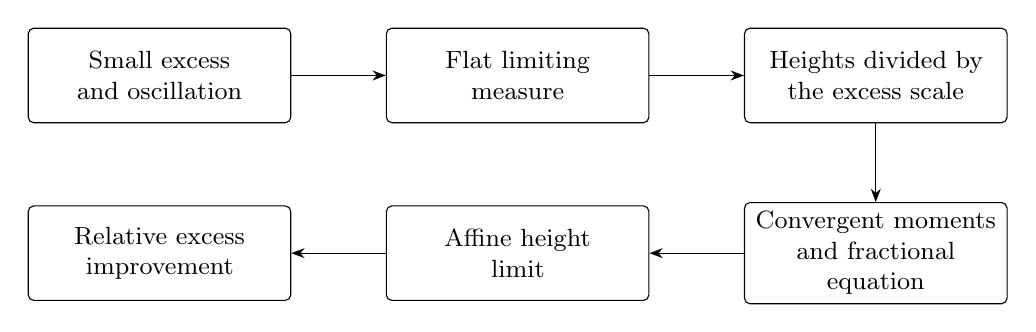
\begin{tikzpicture}[>=Stealth,
 box/.style={draw,rounded corners=2pt,align=center,text width=3.1cm,
 minimum height=1.2cm,font=\small},node distance=1.2cm]
 \node[box] (a) {Small excess\\and oscillation};
 \node[box,right=of a] (b) {Flat limiting\\measure};
 \node[box,right=of b] (c) {Heights divided by\\the excess scale};
 \node[box,below=1cm of c] (d) {Convergent moments\\and fractional equation};
 \node[box,left=of d] (e) {Affine height\\limit};
 \node[box,left=of e] (f) {Relative excess\\improvement};
 \draw[->] (a)--(b); \draw[->] (b)--(c); \draw[->] (c)--(d);
 \draw[->] (d)--(e); \draw[->] (e)--(f);
\end{tikzpicture}
\caption{The second limiting argument retains the size of the incoming
error. Its affine conclusion supplies the improvement needed to
propagate flatness. The independent weighted-rigidity lemma also
identifies the density in the flat limiting measure.}\label{fig:two-limits}
\end{figure}

Finally, start at a flat descendant and follow a chain of cells.
A later cell with large bilateral flatness must have an intervening
oscillation-bad cell. Lemma~\ref{lem:seed-charging} counts these
interventions for an arbitrary finite bad family. This proves
Proposition~\ref{prop:beta-packing}, and the geometric endpoint then
completes Theorem~\ref{thm:main}.

\section{Analytic oscillation and flat seeds}
\label{sec:flat-balls}

This section provides two inputs for the later geometric argument.
Large oscillations of the Riesz pairing occur on a Carleson family of
cubes, and, outside another Carleson family, every cube has a
bilaterally flat descendant at a uniformly bounded depth.  We first prove the oscillation estimate by a Bessel inequality for
mean-zero Lipschitz tests. For the second assertion, two successive
tangents give a local alternative: absence of a flat ball forces a large
annular transform. Differences of local averages then turn that
alternative into a packing estimate.

Throughout the section $1\leq n<d$, and $\mu$ satisfies the
AD regularity and operator hypotheses of Theorem~\ref{thm:main}.
We use the global upper growth constant $G$ from
Lemma~\ref{lem:global-growth}.  Constants may depend on
$d,n,C_{\rm AD},C_{\rm R}$ and the lattice constants; additional
parameters are indicated when they occur.

\subsection{Packing the oscillation tests}

We use the Lipschitz-test and finite-depth Haar Riesz-system estimates
developed in \cite[Section~14]{NazarovTolsaVolberg2014} and include
the estimates with our normalization below. The mean-zero Lipschitz
test estimate and its oscillation-packing consequence also appear in
\cite[Section~5 and Appendix~B]{JayeNazarov2013}.

Write $\mathcal D(Q_0)=\{Q\in\mathcal D:Q\subset Q_0\}$.
We use the Carleson condition \eqref{eq:carleson-definition}, the
oscillation quantity \eqref{eq:oscillation-definition}, and the cell
mass bounds from Proposition~\ref{prop:dyadic-lattice}:
\begin{equation}\label{eq:packing-cell-masses}
 c_1\ell(Q)^n\le\mu(Q)\le C_1\ell(Q)^n.
\end{equation}
For bounded support, the diameter-truncated lattice has at most one
level with $\ell(Q)>D_E$. That level may be included in an exceptional
family at Carleson cost one. No estimate uses infinitely many scales
larger than the support diameter. Put $E^*=E\setminus N$, where $N$ is
the common null set in Proposition~\ref{prop:dyadic-lattice}. Its
partitions and nesting hold exactly on $E^*$. Also $E^*$ is dense in
$E$, since every ball centered on $E$ has positive measure.

\begin{lemma}[Bessel estimate for dyadic tests]\label{lem:dyadic-test-bessel}
Fix $J>1$. For each cube in a finite family $\mathcal A\subset\mathcal D$,
choose one test $\varphi_Q$ from the class defining $W_J(Q)$. There is
$B_J<\infty$, independent of $\mathcal A$ and the choices, such that
\begin{equation}\label{eq:dyadic-test-bessel}
 \sum_{Q\in\mathcal A}
 \frac{\left|\int\varphi_Q u\,d\mu\right|^2}{\ell(Q)^n}
 \le B_J\int |u|^2\,d\mu\qquad(u\in L^2(\mu)).
\end{equation}
For vector-valued $u$ the same constant works with
$\int\varphi_Q u$ replaced by
$\int\varphi_Q\langle e_Q,u\rangle$, where each $|e_Q|\le1$ may be chosen
independently.
\end{lemma}

\begin{proof}
Put $r_Q=\ell(Q)$, $w_Q=r_Q^{n/2}$ and $f_Q=\varphi_Q/w_Q$.
The support and Lipschitz conditions give $|\varphi_Q|\le2J$: compare a
point of its support with a point on the sphere of radius $Jr_Q$ where
the function vanishes. The tests are in $L^1\cap L^2$ by compact support.
If $r_P\le r_Q$, cancellation in $f_P$ gives
\begin{align}
 |\langle f_Q,f_P\rangle|
 &=\left|\int(f_Q(x)-f_Q(z_P))f_P(x)\,d\mu(x)\right|\notag\\
 &\le H_J\frac{r_P}{r_Q}\frac{w_P}{w_Q},
 \qquad H_J=GJ^{n+1}(2J+1)^2.
 \label{eq:gram-cancellation}
\end{align}
Indeed, on the support of $f_P$ the difference is at most
$Jr_P/(r_Qw_Q)$, and
\[
 \int|f_P|\,d\mu\le \frac{2JG(Jr_P)^n}{w_P}.
\]
The symmetric estimate follows by reversing $P,Q$.

A nonzero inner product requires the two support balls to meet. Fix
$Q$ and a finer level $r_P=2^{-k}r_Q$. Every interacting cube $P$ lies
in $B(z_Q,(2J+C_0)r_Q)$, up to its null boundary. Same-level cells are
pairwise disjoint, so \eqref{eq:packing-cell-masses} and global upper
growth imply
\begin{equation}\label{eq:gram-fine-mass}
 \sum_{\substack{P\text{ at this level}\\
                  \langle f_Q,f_P\rangle\ne0}}r_P^n
 \le H'_J r_Q^n,
 \qquad H'_J=c_1^{-1}G(2J+C_0)^n.
\end{equation}
At a coarser level $r_P=2^kr_Q$, the same argument in
$B(z_Q,(2J+C_0)r_P)$ bounds the number of interacting cubes by $H'_J$.
These are estimates in the measure dimension $n$.

Multiply \eqref{eq:gram-cancellation} by $w_P$. Summing first over a
finer level using \eqref{eq:gram-fine-mass}, and then over a coarser level
using its counting bound, gives respectively
\[
 \sum_{r_P=2^{-k}r_Q}|\langle f_Q,f_P\rangle|w_P
 \le H_JH'_J2^{-k}w_Q,
 \qquad
 \sum_{r_P=2^kr_Q}|\langle f_Q,f_P\rangle|w_P
 \le H_JH'_J2^{-k}w_Q.
\]
Zero inner products may be discarded. Summing the geometric series
therefore yields
\[
 \sum_{P\in\mathcal A}|\langle f_Q,f_P\rangle|w_P
 \le4H_JH'_Jw_Q.
\]
For completeness, a symmetric matrix $(a_{QP})$ of nonnegative entries
with $\sum_P a_{QP}w_P\le Bw_Q$ satisfies
\[
 \sum_{Q,P}a_{QP}|t_Qt_P|\le B\sum_Q|t_Q|^2.
\]
This follows by applying
$2|t_Qt_P|\le |t_Q|^2w_P/w_Q+|t_P|^2w_Q/w_P$ and using symmetry.
Apply it to $a_{QP}=|\langle f_Q,f_P\rangle|$. The resulting bound for
$\|\sum_Qt_Qf_Q\|_2^2$ gives \eqref{eq:dyadic-test-bessel} by Hilbert-space
duality, with $B_J=4H_JH'_J$.

For the vector assertion, write $v_Q=\int f_Qu\,d\mu$. Then
$|\langle e_Q,v_Q\rangle|^2\le|v_Q|^2$. Expand the latter in an
orthonormal basis, apply the scalar estimate to each coordinate of $u$,
and sum by Parseval's identity. The constant is unchanged.
\end{proof}

\begin{proposition}[Oscillation packing]\label{prop:oscillation-packing}
For every $J>1$ and $v>0$, the family
\[
 \mathcal O(J,v)=\{Q\in\mathcal D:W_J(Q)>v\ell(Q)^n\}
\]
is Carleson. Its constant depends only on the fixed data, $J$, and $v$.
\end{proposition}

\begin{proof}
Fix $Q_0$, put $L=\ell(Q_0)$, and fix the single outer ball
\[
 S=B(z_{Q_0},(C_0+2)L).
\]
Let $\mathcal A\subset\mathcal O(J,v)\cap\mathcal D(Q_0)$ be finite.
For each selected cube write $r_Q=\ell(Q)$ and choose a witnessing test
$\varphi_Q$ and a unit-bounded direction $e_Q$, so that
\[
 |\langle e_Q,\mathcal R_\mu(\varphi_Q)\rangle|>vr_Q^n.
\]
For $r_Q\le L/(2J)$ the support of the test lies in $S$, and its distance
from $S^c$ is at least $L$. With $\nu=\mu|S$, cancellation gives
\begin{align*}
 \mathcal R_\mu(\varphi_Q)-\mathcal R_\nu(\varphi_Q)
 =\int\varphi_Q(x)\int_{S^c}
 [K_n(x-y)-K_n(z_Q-y)]\,d\mu(y)\,d\mu(x).
\end{align*}
This integral is absolutely convergent. The kernel derivative bound and
upper growth on dyadic annuli give
\[
 \int_{|y-z_Q|\ge L}|y-z_Q|^{-n-1}\,d\mu(y)
 \le C(n)G/L.
\]
Since $|x-z_Q|\le Jr_Q$ on the support and
$\int|\varphi_Q|\,d\mu\le2JG(Jr_Q)^n$, it follows that
\begin{equation}\label{eq:oscillation-outer-error}
 |\mathcal R_\mu(\varphi_Q)-\mathcal R_\nu(\varphi_Q)|
 \le T_J(r_Q/L)r_Q^n,
 \qquad T_J=C(n)G^2J^{n+2}.
\end{equation}
Choose an integer $N\ge1$, depending only on $J,v$ and the fixed data,
with
\[
 2^{-N}\le\min\{(2J)^{-1},\ v/[2(T_J+1)]\}.
\]
If $Q$ lies at least $N$ generations below $Q_0$, its restricted pairing
therefore has magnitude at least $(v/2)r_Q^n$ in the direction $e_Q$.

The same hard-truncated function $R_{\mu,\varepsilon}1_S$ can be used for
all these fine cubes. For each such cube,
\[
 \int\varphi_Q(x)R_{\mu,\varepsilon}1_S(x)\,d\mu(x)
 =\frac12\iint_{S\times S,\ |x-y|>\varepsilon}
  (\varphi_Q(x)-\varphi_Q(y))K_n(x-y)\,d\mu(x)d\mu(y).
\]
As $\varepsilon\downarrow0$ this converges to
$\mathcal R_\nu(\varphi_Q)$. Antisymmetry gives the displayed identity;
Lipschitz cancellation and upper growth make its near-diagonal majorant
integrable. Also $\int\varphi_Q\,d\nu=0$ because the support lies in $S$.
Lemma~\ref{lem:dyadic-test-bessel} and the hard-truncation bound imply
\[
 \sum_{Q\in\mathcal A}
 \frac{\left|\int\varphi_Q\langle e_Q,
                R_{\mu,\varepsilon}1_S\rangle\,d\mu\right|^2}{r_Q^n}
 \le B_J C_{\rm R}^2\mu(S).
\]
Restrict the sum to the fine cubes and pass to the limit in this finite
sum. We obtain
\[
 \sum_{\substack{Q\in\mathcal A\\r_Q\le2^{-N}L}}r_Q^n
 \le4v^{-2}B_JC_{\rm R}^2\mu(S).
\]
Now $\mu(S)\le G(C_0+2)^nL^n\le
G(C_0+2)^nc_1^{-1}\mu(Q_0)$, so
\eqref{eq:packing-cell-masses} bounds the total mass of the fine cubes
by a fixed multiple of $\mu(Q_0)$. At each of the fewer than $N$ remaining
levels, disjointness and containment in $Q_0$ bound the selected masses
by $\mu(Q_0)$. This proves the desired estimate for every finite
$\mathcal A$, hence for the entire family.
\end{proof}

\subsection{Flat descendants outside a Carleson family}

The second packing estimate provides a small flat region inside every
cube outside a Carleson family. The allowed depth depends on the desired
aperture and flatness, but is uniform over all cubes.

\begin{proposition}[Flat seeds outside a Carleson family]\label{prop:flat-seeds}
For every $A_{\rm F}\ge1$ and $\eta>0$ there are an integer $N_{\rm F}\ge1$
and a Carleson family $\mathcal F$ such that every
$Q\in\mathcal D\setminus\mathcal F$ has a proper descendant $P\subset Q$
with
\begin{equation}\label{eq:flat-seed-conclusion}
 1\le\operatorname{depth}_Q(P)\le N_{\rm F},
 \qquad b_\mu(z_P,A_{\rm F}\ell(P))<\eta.
\end{equation}
One may also require
$B(z_P,A_{\rm F}\ell(P))\subset B(z_Q,c_0\ell(Q)/4)$.
The constants are uniform in $Q$ and the top cube used in the Carleson
estimate; they depend only on the fixed data, $A_{\rm F}$ and $\eta$.
\end{proposition}

We prove this proposition by detecting a large annular transform whenever
such a descendant is absent. The next lemma supplies the geometric
alternative independently of the operator bound; the subsequent
comparison of averages makes its annular branch available to a Bessel
estimate.

\subsubsection{The local annular alternative}

The argument follows the flat-ball/large-annulus method of Nazarov,
Tolsa and Volberg; see \cite[Section~10]{NazarovTolsaVolberg2014}.
We give the version needed here in arbitrary codimension, with the
stated smooth annuli and admissible-radius conventions.

Fix a smooth radial function $\chi:\R^d\to[0,1]$ which equals one
on $\overline B(0,1)$ and vanishes outside $B(0,2)$.  For $r>0$ put
$\chi_{a,r}(y)=\chi((y-a)/r)$, and, for $0<r\leq R$, define
\begin{equation}\label{eq:smooth-annular-transform}
 \mathcal S_\mu(a;r,R)
   =\int \bigl(\chi_{a,R}(y)-\chi_{a,r}(y)\bigr)
                 K_n(a-y)\,d\mu(y).
\end{equation}
This is an absolutely convergent vector integral: its integrand is
bounded, compactly supported, and zero near $a$.  The same definition
will be used for any measure with locally finite mass.

\begin{lemma}[A flat ball or a large annulus]\label{lem:annular-alternative}
Fix $0<\kappa<1/8$, $\varepsilon>0$, and $T>0$.  There exists
$\rho\in(0,\kappa)$, depending only on
$d,n,C_{\rm AD},G,\kappa,\varepsilon,T$, with the following property.
For every $a_0\in E$ and $0<s\leq D_E$, at least one of the
following assertions holds:
\begin{enumerate}
\item There are $a\in E\cap B(a_0,\kappa s)$ and
      $\rho s\leq t<\kappa s$ such that
      $b_\mu(a,t)<\varepsilon$.
\item There are $a\in E\cap B(a_0,\kappa s)$ and
      $\rho s\leq r\leq R<\kappa s$ such that
      $|\mathcal S_\mu(a;r,R)|>T$.
\end{enumerate}
The number $\rho$ is chosen before $\mu$, $a_0$, and $s$.
The operator bound is not needed in this lemma.
\end{lemma}

\begin{proof}
We first prove a qualitative assertion for measures with global
upper and lower growth.  We then localize it by taking a tangent and
obtain the uniform radius floor by compactness.

\paragraph{Support convergence and annular bounds.}
We record the elementary convergence facts needed at both stages.
Suppose $\sigma_j$ converge weakly on compact sets to $\sigma$,
have a common upper growth bound, and satisfy
\begin{equation}\label{eq:capped-lower-growth-flat}
 \sigma_j(B(x,t))\geq c t^n
 \qquad(x\in\supp\sigma_j,\quad 0<t\leq h),
\end{equation}
where $c,h>0$ are fixed.  On every bounded region their supports
converge in both directions, with an arbitrarily small enlargement
of that region.  Indeed, if bounded support points $x_j$ stayed a
positive distance from $\supp\sigma$, a subsequence would converge
to such a point $x$.  A continuous cutoff near $x$, together with
\eqref{eq:capped-lower-growth-flat} at a sufficiently small fixed
radius, would have uniformly positive $\sigma_j$ integrals and
zero $\sigma$ integral.  Conversely, a ball about a point of
$\supp\sigma$ contains a nonnegative compactly supported
continuous test with positive $\sigma$ integral.  Its $\sigma_j$
integral is eventually positive.  Finite coverings make both
assertions uniform on bounded sets.  The limit also has lower growth:
for $x\in\supp\sigma$ and $0<t\leq h$, choose $x_j\to x$
and a continuous cutoff equal to one on $B(x,t/2)$ and supported
in $B(x,t)$.  Eventually $B(x_j,t/4)\subset B(x,t/2)$, so passing
the cutoff integrals to the limit gives
$\sigma(B(x,t))\geq c(t/4)^n$.

In particular, if $a_j\in\supp\sigma_j$ tend to
$a\in\supp\sigma$ and the limit is sufficiently flat on
$B(a,2t)$, then the sources are flat on $B(a_j,t)$.
For example, for $0<\eta\leq1$,
\begin{equation}\label{eq:nonflat-limit-flat}
 \left[ b_{\sigma_j}(x,t)\geq\eta
 \text{ for all nearby support centers and all large }j\right]
 \quad\Longrightarrow\quad
 b_\sigma(a,2t)\geq\eta/64.
\end{equation}
To check the numerical slack, if the last inequality failed, choose
an $n$-plane whose sum of deviations on $B(a,2t)$ is
less than $\eta t/32$.  Approximate $a$ by $a_j$ and both supports
within $\eta t/32$.  Points of either set in $B(a_j,t)$ and all
the points used to approximate them then lie in $B(a,2t)$.
Each of the two deviations for the sources is less than
$\eta t/8$, contradicting $b_{\sigma_j}(a_j,t)\geq\eta$.
This reasoning uses only the lower growth at small fixed radii;
the tested radius $t$ need not be below $h$.

For fixed $r,R>0$, the kernel in
\eqref{eq:smooth-annular-transform} is continuous with compact
support.  If its center varies from $a_j$ to $a$, the kernels
converge uniformly and have a common bounded support.  The upper
growth bound therefore gives
\begin{equation}\label{eq:annular-center-convergence}
 \mathcal S_{\sigma_j}(a_j;r,R)
       \longrightarrow \mathcal S_\sigma(a;r,R).
\end{equation}
Here and below support centers in a limit can be approximated by
source support centers, as just proved.

For $u>0$ define the normalized dilation
\[
 \sigma_{a,u}=u^{-n}
       \bigl(y\mapsto (y-a)/u\bigr)_\#\sigma.
\]
A change of variables gives the exact identities
\begin{equation}\label{eq:annular-flat-scaling}
 \begin{split}
 \mathcal S_{\sigma_{a,u}}(b;r,R)
      &=\mathcal S_\sigma(a+ub;ur,uR),\\
 b_{\sigma_{a,u}}(b,t)&=b_\sigma(a+ub,ut).
 \end{split}
\end{equation}
Thus a bound $|\mathcal S_\sigma(x;r,R)|\leq T$ at all support
centers and all positive radii survives dilations and compact
limits.  A global lower bound $b_\sigma\geq\eta$ survives a
compact limit with the loss $\eta\mapsto\eta/64$.
The compactness and nonvanishing of normalized dilations follow
from Lemma~\ref{lem:weak-compactness}: upper growth controls the
mass on each compact set, and lower growth preserves positive mass
in every ball about the origin.

\paragraph{Two tangents reduce the containing dimension.}
Suppose, towards a contradiction, that a nonzero measure $\sigma$
satisfies global bounds
\[
 c t^n\leq\sigma(B(x,t)),\qquad
 \sigma(B(y,t))\leq G_1t^n
 \quad(x\in\supp\sigma,\ y\in\R^d,\ t>0),
\]
that $|\mathcal S_\sigma(x;r,R)|\leq T$ at every support
center and all $0<r\leq R$, and that
$b_\sigma(x,t)\geq\eta>0$ everywhere.  Decreasing $\eta$ if
necessary, assume $\eta\leq1$.  Let $P$ be a linear subspace
containing the support, initially $P=\R^d$.

The support cannot fill $P$.  If it did, upper and lower growth
would force $\dim P=n$.  To see this, write $k=\dim P$ and
cover its unit ball by $O(u^{-k})$ balls of radius $u$.
For $k<n$, upper growth would make its mass tend to zero.
For $k>n$, a family of $\gtrsim u^{-k}$ disjoint balls of
radius comparable to $u$, centered in the unit ball of $P$,
would have total mass $\gtrsim u^{n-k}$, contradicting the
upper bound on a fixed larger ball.  When $k=n$, the support
is an $n$-plane and all its bilateral beta numbers are zero.
Each possibility contradicts the assumptions.

Choose $c_1\in P\setminus\supp\sigma$ and a nearest support
point $a$ to $c_1$.  Such a point exists because the support is
nonempty and closed in finite-dimensional Euclidean space.
Set $e=a-c_1\in P\setminus\{0\}$.  The nearest-point inequality
implies
\[
 2\langle e,y-a\rangle+|y-a|^2\geq0
       \qquad(y\in\supp\sigma).
\]
After dilation at $a$ by scales $u_j\downarrow0$ this becomes
$2\langle e,x\rangle+u_j|x|^2\geq0$.
Pass to a nonzero limit $\tau$.  The support-convergence argument
shows that
\[
 \supp\tau\subset P\cap\{x:\langle e,x\rangle\geq0\},
 \qquad 0\in\supp\tau.
\]
This first tangent retains global upper and lower growth,
the annular bound $T$, and positive global nonflatness.

We next use the sign of the normal kernel to take a second
tangent.  Define
\[
 p_e(x)=\frac{\langle e,x\rangle_+}{|x|^{n+1}}
 \quad(x\ne0),\qquad p_e(0)=0,
 \qquad t_+=\max\{t,0\}.
\]
For $2r\leq R_0$, the weight
$\chi_{0,R_0}-\chi_{0,r}$ is nonnegative everywhere and equals
one when $2r\leq|x|\leq R_0$.  In fact, inside the $R_0$-ball
the outer cutoff is one, and outside it the inner cutoff is zero.
This argument requires no monotonicity of the cutoff.
On the support of $\tau$,
\[
 \int(\chi_{0,R_0}-\chi_{0,r})p_e\,d\tau
       =-\langle e,\mathcal S_\tau(0;r,R_0)\rangle
       \leq |e|T.
\]
Given $v>0$, take $r=\min(v,R_0)/4$ to obtain
\[
 \int_{v<|x|<R_0}p_e(x)\,d\tau(x)\leq |e|T.
\]
Monotone convergence, using $p_e(0)=0$, proves
$p_e\in L^1(\tau|_{B(0,R_0)})$.  This establishes an actual
integrability statement before taking the next limit.

For any fixed $R>0$, exact scaling gives
\begin{align}\label{eq:vanishing-normal-moment}
 \int_{B(0,R)}\langle e,x\rangle_+\,d\tau_{0,u}(x)
  &=u^{-n-1}\int_{B(0,uR)}\langle e,y\rangle_+\,d\tau(y)\notag\\
  &\leq R^{n+1}\int_{B(0,uR)}p_e(y)\,d\tau(y)
       \longrightarrow0 \qquad(u\downarrow0).
\end{align}
The convergence follows from absolute continuity of the integral:
upper growth and $n>0$ give $\tau(B(0,uR))\to0$.
Take a nonzero compact limit $\nu$ of these second dilations.
Testing with nonnegative compact continuous cutoffs times
$\langle e,x\rangle_+$ shows that this continuous nonnegative
function vanishes throughout $\supp\nu$.
The negative normal part already vanishes on every dilated
support.  Hence
\[
 \supp\nu\subset Q:=P\cap e^\perp,
 \qquad \dim Q<\dim P.
\]
The last inequality uses $e\in P\setminus\{0\}$:
$e$ itself is not in $e^\perp$.  Both tangents retain support
in $P$ because their centers lie in $P$.

The new measure is nonzero, satisfies global upper and lower
growth, has annular bound $T$, and has global beta lower bound
at least $\eta/4096$.  For definiteness, the compactness
estimates may multiply the upper constant by $2^n$ and divide
the lower constant by $4^n$ at each tangent; their precise
values are immaterial.  Strong induction on $\dim P$, allowing
these constants and the positive beta threshold to vary, gives
a contradiction.  We have proved that a globally regular,
globally annular-bounded measure has a flat ball at every
prescribed positive tolerance.

\paragraph{Localization and a uniform radius floor.}
Suppose a measure has global upper growth, lower growth only
for $0<t\leq h$, and annular bound $T$ for support centers in
an open set $U$ with $U\cap\supp\sigma\ne\varnothing$,
and outer radii below a positive cap.
If there were no $\eta$-flat ball in $U$ below another positive
cap, take a tangent at any point of $U\cap\supp\sigma$.
Every fixed normalized radius eventually lies below the physical
caps, and bounded normalized centers dilate into $U$.
Equations~\eqref{eq:annular-center-convergence}--
\eqref{eq:annular-flat-scaling} and
\eqref{eq:nonflat-limit-flat} therefore make the annular bound
and a positive beta lower bound global on the tangent.
The lower growth also becomes global, since its normalized cap
is $h/u_j\to\infty$.  This contradicts the preceding paragraph.
Thus the local qualitative alternative holds with no radius floor.

Normalize the statement of the lemma by $a_0=0$, $s=1$.
The resulting measures have common global upper growth, origin
in their supports, and lower growth at all support centers for
$0<t\leq1$.  If no common $\rho$ worked, choose counterexamples
$\mu_j$ with floors $\rho_j\downarrow0$.
The uniform mass bounds on compact sets give a locally weakly
convergent subsequence, by the compactness argument in
Lemma~\ref{lem:weak-compactness}.  The fixed lower bound at zero
keeps its limit $\nu$ nonzero and puts $0\in\supp\nu$.
The support-convergence argument above transfers the lower bound
at radii below a fixed positive cap to $\nu$.  Every fixed annulus with center in $B(0,\kappa)$ and
$0<r\leq R<\kappa$ eventually lies above the floor $\rho_j$.
Its transform on the limit is therefore bounded by $T$.
For every fixed $0<t<\kappa$, the failure of flat balls at
radius $t/2$ and \eqref{eq:nonflat-limit-flat} give
\[
 b_\nu(a,t)\geq\min(\varepsilon,1)/64
 \qquad(a\in\supp\nu\cap B(0,\kappa)).
\]
The local qualitative alternative contradicts these two
properties.  This proves the existence of $\rho$ before the
measure is chosen.  Finally,
\eqref{eq:annular-flat-scaling} transports the conclusion back
to $a_0,s$.  Only the original lower growth below $s\leq D_E$
has been used.
\end{proof}

\subsubsection{From large annuli to flat descendants}

The passage from a large annulus to a difference of local averages,
and then to a packing estimate, follows the mechanism in
\cite[Section~15]{NazarovTolsaVolberg2014}.

The next comparison makes the large-annulus branch of
Lemma~\ref{lem:annular-alternative} usable in an $L^2$ packing argument.
For a positive finite-measure set $A$, write
$\langle u\rangle_A=\mu(A)^{-1}\int_Au\,d\mu$.

\begin{lemma}[Annuli and differences of averages]\label{lem:annular-average-gap}
Let $0<r\le R$, let $S$ be a bounded measurable set containing
$B(a,2R)$, and let $A\subset B$ be measurable sets of positive finite
measure satisfying
\[
 A\subset B(a,r/2),\qquad B\subset B(a,R/2),\qquad
 r^n\le M\mu(A),\qquad R^n\le M\mu(B).
\]
There is a constant
\[
 E_0=3C_{\rm R}(G2^nM)^{1/2}+3C(n)G,
\]
independent of $r,R,R/r,S$ and $\varepsilon$, such that, for every
$0<\varepsilon<r/2$,
\begin{equation}\label{eq:annular-average-error}
 \left|\mathcal S_\mu(a;r,R)
 -\bigl(\langle R_{\mu,\varepsilon}1_S\rangle_A
       -\langle R_{\mu,\varepsilon}1_S\rangle_B\bigr)\right|
 \le E_0.
\end{equation}
In particular, one direction chosen from $\mathcal S_\mu(a;r,R)$
witnesses an average gap at least $|\mathcal S_\mu(a;r,R)|-E_0$
for every such $\varepsilon$.
\end{lemma}

\begin{proof}
Decompose the one fixed input as
\[
 1_S=f+g+h,\qquad
 f=\chi_{a,r},\quad g=\chi_{a,R}-\chi_{a,r},\quad
 h=1_S-\chi_{a,R}.
\]
Here $|g|,|h|\le1$, $g$ vanishes on $B(a,r)$, and $h$ vanishes on
$B(a,R)$. All three functions belong to $L^2(\mu)$. Upper growth gives
\[
 \|f\|_2^2\le G(2r)^n,
 \qquad \|g\|_2^2\le G(2R)^n.
\]
Cauchy--Schwarz and the operator bound consequently bound each of
\[
 |\langle R_{\mu,\varepsilon}f\rangle_A|,
 \quad |\langle R_{\mu,\varepsilon}f\rangle_B|,
 \quad |\langle R_{\mu,\varepsilon}g\rangle_B|
\]
by $C_{\rm R}(G2^nM)^{1/2}$; use $r\le R$ for the middle term.

If $u\in L^2(\mu)$, $|u|\le1$, and $u$ vanishes on $B(a,t)$, then for $|x-a|\le t/2$
and $0<\varepsilon<t/2$ there is no truncation boundary on its support.
The kernel derivative estimate therefore gives
\[
 |R_{\mu,\varepsilon}u(x)-R_{\mu,\varepsilon}u(a)|
 \le C(n)|x-a|\int_{|y-a|\ge t}|y-a|^{-n-1}\,d\mu(y)
 \le C(n)G.
\]
Apply this once to $g$ on $A$, and twice to $h$ on $A$ and $B$.
Since $R_{\mu,\varepsilon}g(a)=\mathcal S_\mu(a;r,R)$, expanding the
two averages of $R_{\mu,\varepsilon}(f+g+h)$ proves
\eqref{eq:annular-average-error}. Finally choose a unit-bounded $e$ with
$\langle e,\mathcal S_\mu(a;r,R)\rangle=|\mathcal S_\mu(a;r,R)|$.
This choice precedes $\varepsilon$; projecting
\eqref{eq:annular-average-error} onto $e$ proves the last assertion.
\end{proof}



\begin{proof}[Proof of Proposition~\ref{prop:flat-seeds}]
Put $L_0=\max\{1,2C_0\}$ and $M=(8L_0)^n/c_1$.
Fix the comparison constant $E_0$ in
Lemma~\ref{lem:annular-average-gap}, with this value of $M$.
Apply Lemma~\ref{lem:annular-alternative} with
\[
 \kappa=c_0/32,\qquad
 \epsilon_{\rm F}=\frac{\eta A_{\rm F}}{32(A_{\rm F}+C_0)},
 \qquad T=E_0+2.
\]
Let $\rho>0$ be its uniform relative radius. These choices, including
$\rho$, are made before the cube $Q$ is chosen. For now assume
$\ell(Q)\le D_E$ and apply that lemma at $a_0=z_Q$, $s=\ell(Q)$.

\smallskip\noindent
\emph{The flat branch produces a seed.}
Suppose the lemma gives $a\in E\cap B(z_Q,\kappa\ell(Q))$ and
$\rho\ell(Q)\le t<\kappa\ell(Q)$ with $b_\mu(a,t)<\epsilon_{\rm F}$.
Choose $b\in E^*\cap B(a,t/8)$, and choose the dyadic scale of $P$ so that
\[
 \frac{t}{16(A_{\rm F}+C_0)}<\ell(P)
 \le\frac{t}{8(A_{\rm F}+C_0)}.
\]
Let $P$ be the cell at that scale containing $b$.
Both $b\in Q$ and $\ell(P)<\ell(Q)$ follow from the core containment
and $t<\kappa\ell(Q)$, so exact nesting on $E^*$ gives $P\subset Q$.
Also $|z_P-b|\le C_0\ell(P)$, whence
\[
 B(z_P,A_{\rm F}\ell(P))\subset B(a,t)
 \cap B(z_Q,c_0\ell(Q)/4).
\]
Choose an affine plane for which the sum of the two deviations in
$B(a,t)$ is less than $\epsilon_{\rm F}t$. Restricting both suprema to
the smaller ball gives
\[
 b_\mu(z_P,A_{\rm F}\ell(P))
 <\frac{\epsilon_{\rm F}t}{A_{\rm F}\ell(P)}
 <\frac{16\epsilon_{\rm F}(A_{\rm F}+C_0)}{A_{\rm F}}
 =\eta/2.
\]
The lower bound for $t$ bounds the depth of $P$ uniformly. For example,
any integer $N_{\rm F}>\log_2(16(A_{\rm F}+C_0)/\rho)$ suffices.

\smallskip\noindent
\emph{Cubes without a flat seed have a large annulus.}
Let $\mathcal F_1$ be the cubes with $\ell(Q)\le D_E$ for which no seed
as in \eqref{eq:flat-seed-conclusion}, with the additional ball
containment, exists at depth at most $N_{\rm F}$. They must lie in the
annular branch. Thus each has radii
\[
 \rho\ell(Q)\le r_Q\le R_Q<\kappa\ell(Q)
\]
and a center $a_Q$ in the same core with
$|\mathcal S_\mu(a_Q;r_Q,R_Q)|>E_0+2$.
For these fixed positive radii the annular transform is continuous in
its center. Indeed the annular kernel is zero near its center, is
continuous there after extension by zero, and has bounded compact
support locally uniformly in the center; dominated convergence applies
using local finiteness. Density of $E^*$ therefore permits replacing
$a_Q$ by $a'_Q\in E^*$ so close that
\[
 |a'_Q-z_Q|<2\kappa\ell(Q),\qquad
 |\mathcal S_\mu(a'_Q;r_Q,R_Q)|>E_0+1.
\]
This perturbation uses the strict core and norm margins, and does not
change either radius.

Choose dyadic scales $s_r,s_R$ with
\[
 \frac{r_Q}{8L_0}<s_r\le\frac{r_Q}{4L_0},\qquad
 \frac{R_Q}{8L_0}<s_R\le\frac{R_Q}{4L_0},
\]
using the same monotone rounding rule, so $s_r\le s_R$.
Let $A_Q$ and $B_Q$ be the cells at those scales containing $a'_Q$.
They are descendants of $Q$ with $A_Q\subset B_Q\subset Q$.
Since a cell at scale $s$ has diameter at most $L_0s$,
\[
 A_Q\subset B(a'_Q,r_Q/2),\qquad
 B_Q\subset B(a'_Q,R_Q/2),
 \quad r_Q^n\le M\mu(A_Q),\quad R_Q^n\le M\mu(B_Q).
\]
Fix an integer $I\ge1$ larger than $\log_2(8L_0/\rho)$.
The depth of $A_Q$ below $Q$ is at most $I$, and
\begin{equation}\label{eq:haar-inner-parent-mass}
 \mu(Q)\le H_I\mu(A_Q),\qquad
 H_I=(C_1/c_1)2^{In}.
\end{equation}
Neither $M$ nor $E_0$ depends on $\rho$; the depth cost $H_I$ is allowed
to depend on the now fixed $\rho$.

\smallskip\noindent
\emph{Haar Bessel gives the Carleson estimate.}
Set
\[
 h_Q=\mu(A_Q)^{1/2}
       \left(\frac{1_{A_Q}}{\mu(A_Q)}-
             \frac{1_{B_Q}}{\mu(B_Q)}\right).
\]
Direct integration gives $\int h_Q\,d\mu=0$ and
$\|h_Q\|_2^2=1-\mu(A_Q)/\mu(B_Q)\le1$.
This function is supported in $Q$ and is constant almost everywhere on
every cell at least $I$ generations below $Q$.
Partition a finite collection of these functions according to the
level of $Q$ modulo $I$. Within one class, distinct equal-level parents
are disjoint. For unequal levels, the gap is at least $I$: the coarser
function is constant on the finer parent, or their supports are
disjoint. The finer function's mean zero gives orthogonality. Bessel's
inequality in each class and summation give
\begin{equation}\label{eq:bounded-depth-haar-bessel}
 \sum_Q\left|\int h_Q\langle e_Q,u\rangle\,d\mu\right|^2
 \le I\|u\|_2^2
\end{equation}
for vector $u\in L^2(\mu)$ and independently chosen $|e_Q|\le1$.
The vector extension follows by the same Parseval argument as in
Lemma~\ref{lem:dyadic-test-bessel}.

Fix a top cube $Q_0$ and a finite
$\mathcal A\subset\mathcal F_1\cap\mathcal D(Q_0)$. Use, for every
selected cube, the same set
$S=B(z_{Q_0},(C_0+2)\ell(Q_0))$.
The annular center and radius bounds ensure
$B(a'_Q,2R_Q)\subset S$.
Choose $e_Q$ from the annular vector as in
Lemma~\ref{lem:annular-average-gap}; then choose a single
\[
 0<\varepsilon<\tfrac12\min_{Q\in\mathcal A}r_Q
\]
when the family is nonempty. The average gap is greater than one for
every selected $Q$ at this same truncation. Consequently
\[
 \mu(A_Q)
 <\left|\int h_Q
       \langle e_Q,R_{\mu,\varepsilon}1_S\rangle\,d\mu\right|^2.
\]
By \eqref{eq:haar-inner-parent-mass},
\eqref{eq:bounded-depth-haar-bessel}, and the operator bound,
\[
 \sum_{Q\in\mathcal A}\mu(Q)
 \le H_I I C_{\rm R}^2\mu(S)
 \le H_I I C_{\rm R}^2
       \frac{G(C_0+2)^n}{c_1}\mu(Q_0).
\]
The empty family is immediate. Taking the supremum over finite
subfamilies proves that $\mathcal F_1$ is Carleson. Finally add the possible top level with $\ell(Q)>D_E$ to obtain
$\mathcal F$. Its mass below any top cube is at most the mass of that
top cube. The seed conclusion and its uniform depth bound
hold for every cube outside this family.
\end{proof}

\section[Reflectionless limits and normal coordinates]{Reflectionless limits and compatible normal coordinates}
\label{sec:planar-limits}

We first compare two planes using points near both of them. This gives one
reference plane that controls the errors over a finite range of dyadic radii.
We then identify the
measure obtained when those errors vanish.  Three assertions enter that
identification separately: the limit is supported in a plane, its support
fills the plane, and its density on that plane is constant.

\subsection{Comparison from measured errors}

\begin{lemma}[Comparison of fitting planes]\label{lem:plane-comparison}
Fix $1\le n\le d$, $G\ge0$, and $c>0$.  There are constants
$A>0$ and $0<\varepsilon_0\le1$, depending only on $n,d,G,c$, with the
following property.  Suppose that $\sigma$ has global upper $n$-growth $G$,
$R>0$, and $\sigma(B(0,R))\ge cR^n$.  If $S,W$ are affine $n$-planes and
$0<\eta\le\varepsilon_0R$ satisfy
\begin{equation}\label{eq:joint-plane-error}
 \int_{B(0,R)}\bigl(\dist(x,S)^2+\dist(x,W)^2\bigr)\,d\sigma(x)
 \le \frac c2\eta^2R^n,
\end{equation}
then
\begin{align}
 \dist(x,W)&\le A\eta(1+|x|/R) &&(x\in S),\label{eq:plane-comparison}\\
 |\dist(x,S)-\dist(x,W)|&\le A\eta(3+|x|/R)
       &&(x\in\R^d).\label{eq:distance-comparison}
\end{align}
The first conclusion also holds with $S$ and $W$ interchanged.
\end{lemma}

\begin{proof}
Every integral in \eqref{eq:joint-plane-error} is finite, since its integrand
is bounded on the ball and upper growth implies local finiteness.  Markov's
inequality shows that
\[
 F=\{x\in B(0,R):\dist(x,S)^2+\dist(x,W)^2<\eta^2\}
 \quad\hbox{satisfies}\quad \sigma(F)\ge(c/2)R^n.
\]
In particular, every point of $F$ is within $\eta$ of both planes.

Here is the quantitative nonconcentration needed to choose points in $F$.
If $V$ is an affine $k$-plane, $k<n$, and $0<\tau\le1$, then
\begin{equation}\label{eq:lower-dimensional-tube}
 \sigma\{x\in\overline B(0,R):\dist(x,V)<\tau R\}
 \le G2^n3^k\tau R^n.
\end{equation}
Indeed, projection onto $V$, centered at the projection of $0$, sends
$\overline B(0,R)$ into its intrinsic closed $R$-ball.  A maximal
$\tau R$-separated subset of this intrinsic ball has at most
$(1+2/\tau)^k$ points: its disjoint open $\tau R/2$-balls lie in the
$(R+\tau R/2)$-ball, and comparison of their $k$-dimensional volumes gives
this bound.  Maximality gives a $\tau R$-net.  Ambient balls of radius
$2\tau R$ about its points cover the indicated tube.  Upper growth gives
$G2^n3^k\tau^{n-k}R^n$, which implies
\eqref{eq:lower-dimensional-tube}.

Choose
\[
 \tau=\min\{1,c/[4(G2^n3^n+1)]\}.
\]
The tube mass in \eqref{eq:lower-dimensional-tube} is strictly less than
$(c/2)R^n$.  Thus we can successively choose
$p_0,\ldots,p_n\in F\cap\supp\sigma$ such that, for $1\le j\le n$,
\[
 \dist\bigl(p_j,p_0+\operatorname{span}
              \{p_i-p_0:1\le i<j\}\bigr)\ge\tau R.
\]
At each step the affine span has dimension less than $n$, and $\supp\sigma$
has full measure.  Put $v_j=p_j-p_0$.  Then $|v_j|\le2R$.  These vectors
satisfy
\begin{equation}\label{eq:anchor-conditioning}
 \sum_{j=1}^n|t_j|\le \frac KR\left|\sum_{j=1}^nt_jv_j\right|,
\end{equation}
where $K$ depends only on $n,\tau$.  For completeness, define
$K_0=0$ and $K_{j+1}=K_j(1+2/\tau)+1/\tau$.
Projection perpendicular to the span of the first $j$ vectors bounds the
last coefficient by the norm of the complete linear combination divided
by $\tau R$.  Subtracting its last term enlarges that norm by at most
$1+2/\tau$.  Induction proves \eqref{eq:anchor-conditioning} with $K=K_n$.
It also proves independence of the $v_j$.

Let $a=\pi_Sp_0$ and $w_j=\pi_Sp_j-a$, where $\pi_S$ is orthogonal
projection.  We have $|w_j-v_j|\le2\eta$.  If
$\eta/R\le1/[4(K+1)]$, \eqref{eq:anchor-conditioning} and absorption give
\[
 \sum|t_j|\le\frac{2K}{R}\left|\sum t_jw_j\right|.
\]
The $n$ vectors $w_j$ consequently form a basis of the direction of $S$.
Every projected anchor $a,a+w_1,\ldots,a+w_n$ lies within $2\eta$ of $W$.
The orthogonal normal-coordinate map for $W$ is affine and has norm
$\dist(\cdot,W)$.  Applying this affine map to
$x=a+\sum t_jw_j$ gives
\[
 \dist(x,W)\le2\eta+4\eta\sum|t_j|
 \le2\eta+\frac{8K\eta}{R}|x-a|.
\]
Since $|a|\le R+\eta\le2R$, this proves
\eqref{eq:plane-comparison}, for example with
$A=2(1+8K)$ and
$\varepsilon_0=\min\{1,1/[4(K+1)]\}$.
All choices preceded $\sigma,R,S,W,\eta$.

Finally, for arbitrary $x$, let $p=\pi_Sx$.  Since
$|\pi_S0|\le|a|\le2R$ and the linear part of $\pi_S$ is a contraction,
$|p|\le|x|+2R$.  Hence
\[
 \dist(x,W)\le|x-p|+\dist(p,W)
 \le\dist(x,S)+A\eta(3+|x|/R).
\]
Interchanging the planes proves \eqref{eq:distance-comparison}.
\end{proof}

\begin{lemma}[One reference plane through a finite horizon]
\label{lem:fixed-plane-moments}
Fix $0<\gamma<1/2$ and the constants $n,d,G,c$ of
Lemma~\ref{lem:plane-comparison}.  There are $\kappa>0$ and $M<\infty$,
depending only on these data and $\gamma$, as follows.  Suppose $K\ge0$ is
an integer, $\delta>0$, $\delta2^{\gamma K}\le\kappa$, $\sigma$ has
global upper growth $G$, and, for $0\le k\le K$,
\[
 \sigma(B(0,2^k))\ge c2^{kn},
 \qquad e_\sigma(0,2^k)\le\delta2^{\gamma k}.
\]
Then an affine $n$-plane $S$ satisfies
\begin{equation}\label{eq:fixed-plane-moments}
 \int_{B(0,2^k)}\dist(x,S)^2\,d\sigma(x)
 \le M\delta^2 2^{k(n+2+2\gamma)}
 \qquad(0\le k\le K).
\end{equation}
\end{lemma}

\begin{proof}
Write $b=2^\gamma>1$ and $R_i=2^i$.  The definition of the infimum in
$e_\sigma$ and the positivity of $\delta b^i$ give affine planes $P_i$,
$0\le i\le K$, with
\[
 \int_{B(0,R_i)}\dist(x,P_i)^2\,d\sigma
 \le2(\delta b^i)^2R_i^{n+2}.
\]
No attainment of a least-squares infimum is required.  For $0\le i<K$,
restricting the error for $P_{i+1}$ to $B(0,R_i)$ shows that the sum of neighboring errors
is at most
$D(\delta b^i)^2R_i^{n+2}$, where
$D=2+2\cdot2^{n+2}b^2$.
Choose $L>0$ with $D\le L^2c/2$, and put
$\eta_i=L\delta R_i b^i$.  Taking
$\kappa=\varepsilon_0/L$ ensures $\eta_i\le\varepsilon_0R_i$ through
the horizon.  Lemma~\ref{lem:plane-comparison} gives, at the same arbitrary
point $x$ in each step,
\[
 \dist(x,P_i)\le\dist(x,P_{i+1})
       +AL\delta b^i(3R_i+|x|).
\]
For $|x|\le R_k$, the sum of these errors for $i<k$ is bounded by
$B\delta R_kb^k$, where
\[
 B=AL\left(\frac3{2b-1}+\frac1{b-1}\right).
\]
Indeed, sum the geometric series with ratios $2b$ and $b$ separately.
Consequently
$\dist(x,P_0)\le\dist(x,P_k)+B\delta R_kb^k$ on that ball.
Squaring, integrating, and using upper growth proves
\eqref{eq:fixed-plane-moments} with $S=P_0$ and $M=4+2GB^2$.
\end{proof}

\subsection{Rigidity on the limiting plane}

We shall use the symmetric fractional operator
\begin{equation}\label{eq:fractional-operator-definition}
 \mathcal Lg(x)=\int_{\R^n}
 \frac{2g(x)-g(x+z)-g(x-z)}{2|z|^{n+1}}\,dz,
 \qquad g\in C_c^\infty(\R^n).
\end{equation}
This integral is absolutely convergent: the numerator is $O(|z|^2)$ near
zero and is bounded at infinity. Lemma~\ref{lem:fractional-rigidity}
proves that a measurable function $v:\R^n\to\R$ satisfying
$\int|v(x)|(1+|x|)^{-n-2}\,dx<\infty$ and
$\int v\mathcal Lg=0$ for every compact smooth mean-zero test is affine
almost everywhere. If $v$ is essentially bounded, it is constant
almost everywhere.
That lemma concerns functions on $\R^n$ and is proved independently
of the limiting measures constructed here.

\begin{lemma}[Rigidity of a planar reflectionless measure]
\label{lem:planar-rigidity}
Let $1\le n\le d$, let $L$ be an affine $n$-plane, and let $\sigma$ be a
nonzero Radon measure on $\mathbb R^d$ supported in $L$.  Suppose that
$c,G>0$ and
\[
 \sigma(B(x,r))\le Gr^n\quad(x\in\mathbb R^d,\ r>0),
 \qquad
 \sigma(B(x,r))\ge cr^n\quad(x\in\supp\sigma,\ r>0).
\]
Suppose also that $\mathcal R_\sigma(\varphi)=0$ for every compactly
supported Lipschitz function $\varphi$ with $\int\varphi\,d\sigma=0$.
Assume the hard Riesz truncations are uniformly bounded on $L^2(\sigma)$.
Then
\[
 \supp\sigma=L,
 \qquad \sigma=\theta\,\mathcal H^n\!\restriction L
 \quad\text{for some }\theta>0.
\]
The same conclusion holds if the operator assumption on $\sigma$ is
replaced by the following source assumption: $\sigma_j$ are Radon
measures on $\mathbb R^d$ converging to $\sigma$ against compact continuous
tests, with a common global upper $n$-growth bound and a common uniform
hard-truncation $L^2$ bound.  With the Euclidean normalization of
$\mathcal H^n$, the resulting constant satisfies
$c/\omega_n\le\theta\le G/\omega_n$, where
$\omega_n=|B_{\mathbb R^n}(0,1)|$.
\end{lemma}

\begin{proof}
An affine isometry identifies $L$ with $\mathbb R^n$.  Under this
identification write $\mu$ for $\sigma$.  The kernel and its scalar
projections commute with this isometry.  Reflectionlessness passes to
$\mu$ with its actual measure: extend an intrinsic compact Lipschitz test
by composing with orthogonal projection and multiplying by an ambient
compact cutoff equal to one on its trace support.  Its integral is
unchanged.  Choose a localization ball containing the extension and use
the localization independence of the mean-zero pairing from
Lemma~\ref{lem:pairings}.  Thus no density or full-support assertion is
needed to make this identification.

\emph{Full support.}
We first derive an annular bound using only growth and
reflectionlessness.  For a test supported in $\overline B(a,R/2)$, denote by
$P_{a,R}(\varphi)$ the vector expression
\begin{align*}
 &\frac12\iint_{B(a,R)^2}
 K_n(x-y)\bigl(\varphi(x)-\varphi(y)\bigr)\,d\mu(x)d\mu(y)\\
 &\qquad+\int_{B(a,R)}\varphi(x)
 \int_{B(a,R)^c}\bigl[K_n(x-y)-K_n(a-y)\bigr]\,d\mu(y)d\mu(x).
\end{align*}
Both terms are absolutely integrable by the Lipschitz cancellation near
the diagonal and the extra power of decay in the exterior difference.
This expression is defined without a mean-zero assumption; on mean-zero
tests it equals $\mathcal R_\mu$.  Splitting the larger ball into the
smaller ball and its complement, and using oddness, gives
\begin{equation}\label{eq:planar-radius-difference}
 P_{a,R}(\varphi)-P_{a,r}(\varphi)
 =\left(\int\varphi\,d\mu\right)
   \int_{B(a,R)\setminus B(a,r)}K_n(a-y)\,d\mu(y)
\end{equation}
when $0<r\le R$ and $\supp\varphi\subset\overline B(a,r/2)$.
One may first perform the splitting with a finite outer cutoff; the
integrable exterior differences justify its removal.

Choose a nonnegative Lipschitz bump equal to one on $B(a,s)$ and zero
outside $B(a,2s)$, and divide it by its $\mu$-integral.  For $a\in\supp\mu$
the resulting function $\eta_s$ has integral one and satisfies
\[
 \|\eta_s\|_\infty\le (cs^n)^{-1},\qquad
 \Lip(\eta_s)\le (cs^{n+1})^{-1},\qquad
 |P_{a,4s}(\eta_s)|\le C_n(G^2/c+G)=:A.
\]
For the last estimate the interior term is at most a constant times
$(cs^{n+1})^{-1}(Gs^n)(Gs)$; the exterior term is at most a constant
times $Gs/s$, since $\int\eta_s\,d\mu=1$.
Apply reflectionlessness to $\eta_{r/4}-\eta_{R/4}$ and then use
\eqref{eq:planar-radius-difference}.  It follows that
\[
 \left|\int_{B(a,R)\setminus B(a,r)}K_n(a-y)\,d\mu(y)\right|
 \le 2A\qquad(0<r\le R).
\]
Letting inner radii decrease strictly to $\varepsilon$ gives the same
bound on $\{y:\varepsilon<|y-a|<R\}$.  At fixed
$\varepsilon>0$ the kernel is integrable there, so this passage does not
require zero mass on spheres.

Suppose now that $z\notin\supp\mu$, and let $a$ be a nearest support
point to $z$.  Translate $a$ to zero and put $e=a-z\ne0$.
The nearest-point property gives
\[
 2\langle e,x\rangle+|x|^2\ge0\qquad(x\in\supp\mu).
\]
Define
$p_e(x)=\max(0,\langle e,x\rangle)/|x|^{n+1}$ for $x\ne0$,
and set $p_e(0)=0$.  Then
\[
 p_{-e}(x)\le\tfrac12|x|^{1-n},\qquad
 p_e(x)=\langle e,K_n(x)\rangle+p_{-e}(x).
\]
Upper growth makes the first majorant integrable on bounded balls: its
integral on $B(0,R)$ is at most $C_nGR$, as follows by dyadic annuli.
The signed annular bound therefore bounds the nonnegative truncated
integrals of $p_e$ on $B(0,1)$ uniformly.  Monotone convergence proves
$p_e\in L^1(\mu|_{B(0,1)})$.

Take a weakly convergent subsequence of the normalized blowups
$\mu_r(A)=r^{-n}\mu(rA)$ as $r\downarrow0$.
Upper growth supplies compactness, and the lower bound at zero makes the
limit $\tau$ nonzero.  These are the conclusions of
Lemma~\ref{lem:weak-compactness}, applied to the blowups.  The rescaled
quadratic inequality is
$2\langle e,x\rangle+r|x|^2\ge0$; hence
$\supp\tau\subset\{\langle e,x\rangle\ge0\}$.
For every fixed $T>0$,
\[
 \int_{B(0,T)}\max(0,\langle e,x\rangle)\,d\mu_r(x)
 \le T^{n+1}\int_{B(0,rT)}p_e(y)\,d\mu(y)\longrightarrow0.
\]
Testing with compact nonnegative cutoffs shows that $\tau$ is also
supported in $\{\langle e,x\rangle\le0\}$.  It is consequently supported
on a proper hyperplane in $\mathbb R^n$.  This is impossible for a
nonzero measure with upper $n$-growth: covering open sets by disjoint
dyadic cubes and enclosing each cube in a ball shows that such a measure
is bounded above by $C_nG'\,dx$, where $G'$ is its growth constant.
A proper hyperplane has Lebesgue measure zero.  This contradiction proves
$\supp\mu=\mathbb R^n$.

\emph{A positive bounded density.}
The same cube comparison gives $\mu=f\,dx$ with $f\le C_nG$ almost
everywhere.  Full support makes the lower ball bound valid at every
point.  Lebesgue differentiation then gives $f\ge c/\omega_n$ almost
everywhere.  Choose a measurable representative with
\begin{equation}\label{eq:planar-two-sided-density}
 0<c_1\le f(x)\le C_1<\infty\qquad(x\in\mathbb R^n).
\end{equation}
Changing $f$ on a null set has not changed $\mu$.

\emph{A local representative for the pairing.}
Fix a unit direction $u\in\mathbb R^n$, a center $a$, and radii
$0<H$ and $2H\le R$.  Put $B=B(a,R)$ and
\[
 T_{\varepsilon,B}1(x)=\int_B
 \frac{\langle u,x-y\rangle}{\max(\varepsilon,|x-y|)^{n+1}}\,d\mu(y).
\]
There is a constant $D_1$, independent of $B$ and $\varepsilon>0$, such
that
\begin{equation}\label{eq:planar-local-cap-bound}
 \|T_{\varepsilon,B}1\|_{L^2(\mu|_B)}
 \le D_1\mu(B)^{1/2}.
\end{equation}
For the direct operator hypothesis, subtract the hard truncation.
The error kernel is bounded by
$\varepsilon^{-n}\mathbf1_{\{|x-y|\le\varepsilon\}}$.
Its row and column integrals are at most $2^nG$, so Schur's inequality
gives \eqref{eq:planar-local-cap-bound} from the original operator bound.
Restricting the hard operator to a ball preserves that bound, by extending
the input by zero.

Here is also the justification under the source assumption.  Work first
in $\mathbb R^d$ on the ambient ball corresponding to $B$.  Its boundary
has $\sigma$-measure zero by \eqref{eq:planar-two-sided-density}.
Restricted source measures therefore converge weakly as finite measures.
The same Schur estimate gives uniformly bounded capped bilinear pairings
on every source restriction.  For fixed $\varepsilon>0$ these pairings
pass to the limit against two bounded continuous tests: the capped kernel
is bounded continuous, as are the squared tests giving their $L^2$
norms.  Take the input test to be one and the other test to be the capped
output for the limiting finite measure.  That output is bounded
continuous, by dominated convergence at this fixed cap.  The resulting
bilinear estimate gives its genuine $L^2$ bound
\eqref{eq:planar-local-cap-bound}.  Isometric pullback gives precisely the
displayed intrinsic transform.  This argument passes no singular kernel
through weak convergence.

Choose a subsequence $\varepsilon_j\downarrow0$ along which
$T_{\varepsilon_j,B}1$ converges weakly in $L^2(\mu|_B)$ to $v$.
This one subsequence works against every test in that Hilbert space.
Oddness gives, for bounded Lipschitz $\varphi$,
\[
 \int_B T_{\varepsilon,B}1\,\varphi\,d\mu
 =\frac12\iint_{B^2}
 \frac{\langle u,x-y\rangle(\varphi(x)-\varphi(y))}
      {\max(\varepsilon,|x-y|)^{n+1}}\,d\mu(x)d\mu(y).
\]
Removing the cap on the right changes the integral by at most
$C_nG\Lip(\varphi)\mu(B)\varepsilon$.  Thus $v$ represents the actual
interior singular pairing.  On $B(a,H)$ the function
\[
 F(x)=\int_{B(a,R)^c}
 \langle u,K_n(x-y)-K_n(a-y)\rangle\,d\mu(y)
\]
is well defined and bounded: the kernel difference is at most
$C_n|x-a||y-a|^{-n-1}$, whose exterior integral is at most
$C_nG|x-a|/R$.  Fubini now identifies the scalar component of
$\mathcal R_\mu(\varphi)$ with $\int(v+F)\varphi\,d\mu$ for mean-zero
compact Lipschitz tests supported in $B(a,H)$.

Choose a compact Lipschitz test $\eta$ supported in $B(a,H)$ with
$\int\eta\,d\mu=1$, using the positive mass of that ball, and put
$b=\int(v+F)\eta\,d\mu$.  For any smooth compact test $q$ in this smaller
ball, reflectionlessness applied to
$q-(\int q\,d\mu)\eta$ gives
$\int(v+F-b)q\,d\mu=0$.
Since $\mu=f\,dx$, the fundamental lemma for locally integrable functions
applied to $(v+F-b)f$ proves
\begin{equation}\label{eq:planar-local-constant}
 v+F=b\quad\text{$\mu$-almost everywhere on }B(a,H).
\end{equation}
This is a statement about the transform; constancy of $f$ has not yet
been used or proved.

\emph{An unweighted equation and density constancy.}
Let $g\in C_c^\infty(B(a,H))$ be real with $\int g\,dx=0$.
By \eqref{eq:planar-two-sided-density}, $g/f$ belongs to
$L^2(\mu|_B)$.  It is therefore an allowed test for the weak convergence,
even though it need not be Lipschitz.  Moreover, $\mu$ and Lebesgue measure
have the same null sets.  Testing with $g/f$ and using
\eqref{eq:planar-local-constant} yields
\begin{equation}\label{eq:planar-unweighted-local}
 \lim_j\left[\int g(x)T_{\varepsilon_j,B}1(x)\,dx
                   +\int g(x)F(x)\,dx\right]=0.
\end{equation}
The subsequence and $b$ were selected before $g$.

For a compact smooth function $g$, define the scalar test transform
\[
 R_ug(x)=-\frac12\int_{\mathbb R^n}
 \frac{\langle u,h\rangle[g(x+h)-g(x-h)]}{|h|^{n+1}}\,dh.
\]
The integral is absolutely convergent: the first difference is
$O(|h|)$ near zero, and the translated compact supports control infinity.
The analogous capped expression equals the capped transform of $g$ by
translation and reflection.  It converges pointwise to $R_ug$ and is
uniformly bounded on bounded $x$-sets.  If $\supp g\subset B(a,H)$ and
$\int g=0$, then for $|x-a|\ge2H$ and $\varepsilon\le H$ the cap is
inactive and mean-zero cancellation gives
\[
 |R_{u,\varepsilon}^{\rm cap}g(x)|
 \le C_n H\|g\|_1|x-a|^{-n-1}.
\]
Together these bounds form an integrable majorant independent of small
$\varepsilon$.  Since $f$ is bounded, dominated convergence applies to
$\int f R_{u,\varepsilon}^{\rm cap}g$.

For $\varepsilon\le H$, oddness and Fubini identify the expression in
brackets in \eqref{eq:planar-unweighted-local} with
$-\int f R_{u,\varepsilon}^{\rm cap}g\,dx$.
The local capped product is absolutely integrable.  For the exterior
term, use the centered kernel difference, which is absolutely integrable
against $|g(x)|\,dx\,d\mu(y)$; cancel the center term using $\int g=0$
inside the $x$-integral before integrating over the infinite exterior.
The open ball and its closed exterior are exact complements.  Thus no
separate divergent exterior integral or omitted boundary term occurs.
It follows that
\begin{equation}\label{eq:planar-density-riesz}
 \int_{\mathbb R^n}f(x)R_ug(x)\,dx=0
 \qquad\left(g\in C_c^\infty(\mathbb R^n),\ \int g=0\right).
\end{equation}
The ball may be chosen after the test, so this statement has no fixed
support restriction.

Let $u_1,\ldots,u_n$ be an orthonormal basis and
$\psi\in C_c^\infty(\mathbb R^n)$ be real.  Each
$g_i=\partial_{u_i}\psi$ has integral zero.  We claim
\begin{equation}\label{eq:planar-riesz-gradient}
 \sum_{i=1}^nR_{u_i}(\partial_{u_i}\psi)(x)=\mathcal L\psi(x).
\end{equation}
Indeed, set
\[
 Q_x(t)=\int\frac{\psi(x+th)+\psi(x-th)-2\psi(x)}{|h|^{n+1}}\,dh.
\]
Scaling gives $Q_x(t)=tQ_x(1)$ for $t>0$.  Differentiation under the
integral at $t=1$ is justified by second-derivative cancellation near
zero; for $1/2\le t\le2$ the derivative integrand vanishes for all
sufficiently large $|h|$ at fixed $x$.  Consequently
\[
 Q_x(1)=\int\frac{D\psi(x+h)h-D\psi(x-h)h}{|h|^{n+1}}\,dh.
\]
Expand $h$ in the orthonormal basis and use the definition of $R_u$ to
obtain \eqref{eq:planar-riesz-gradient}.  Every pairing with bounded $f$
is integrable by the preceding estimates.  Summing
\eqref{eq:planar-density-riesz} therefore gives
\[
 \int f\mathcal L\psi\,dx=0\qquad(\psi\in C_c^\infty(\mathbb R^n)).
\]
Real and imaginary parts give the same identity for complex tests.
Boundedness supplies $\int|f(x)|(1+|x|)^{-n-2}\,dx<\infty$.
Lemma~\ref{lem:fractional-rigidity} now makes $f$ affine almost everywhere.
A bounded affine function is constant: any nonzero linear part is
unbounded along a line, and continuity promotes an almost-everywhere
bound to an everywhere bound.  Thus $f=\theta$ almost everywhere, with
$\theta>0$ by \eqref{eq:planar-two-sided-density}.  The original ball
bounds give $c\le\theta\omega_n\le G$, completing the proof.
\end{proof}

\subsection{A common flat limit and its normal coordinates}

The passage from vanishing mean-zero pairings to a reflectionless weak
limit is part of the compactness method of Jaye and Nazarov
\cite{JayeNazarov2018I}. Here the common growth bounds control the
singular diagonal and exterior tails, as proved in
Lemma~\ref{lem:weak-compactness}. We combine that local argument with
the measured plane errors; we do not invoke a classification of
arbitrary higher-codimension reflectionless measures.

\begin{proposition}[The flat limit]\label{prop:flat-limit}
Fix $1\le n<d$, $c>0$, $0<G<\infty$, $0\le D_0<\infty$, and
$0<\gamma<1/2$.  Let $\mu_j$ be Radon measures on $\R^d$ with
$0\in E_j=\supp\mu_j$, global upper $n$-growth $G$, and
\[
 \mu_j(B(x,r))\ge cr^n
 \quad(x\in E_j,\ 0<r\le\diam E_j).
\]
Assume every hard-truncated Riesz transform on $L^2(\mu_j)$ has norm at
most $D_0$.  Let $\delta_j>0$, integers $K_j\ge0$, and $A_j,v_j>0$
satisfy
\begin{equation}\label{eq:flat-limit-horizons}
 \begin{gathered}
 \delta_j\longrightarrow0,\quad K_j\longrightarrow\infty,\quad
 \delta_j2^{\gamma K_j}\longrightarrow0,\\
 2^{K_j}\le\diam E_j,\quad A_j\longrightarrow\infty,\quad v_j\longrightarrow0.
 \end{gathered}
\end{equation}
Suppose
\begin{equation}\label{eq:flat-limit-source-excess}
 e_{\mu_j}(0,2^k)\le\delta_j2^{\gamma k}
 \qquad(0\le k\le K_j)
\end{equation}
and
\begin{equation}\label{eq:flat-limit-source-oscillation}
 |\mathcal R_{\mu_j}(\varphi)|\le v_j
 \quad\text{if }\ \Lip\varphi\le1,\quad
 \supp\varphi\Subset B(0,A_j),\quad\int\varphi\,d\mu_j=0.
\end{equation}
There is a subsequence, relabeled by $j$, with the following properties.
All the input sequences are restricted along this same subsequence when
we relabel them.
For each index there are an affine plane
$S_j=a_j+L_j(\R^n)$, tangent and normal linear isometries
\[
 L_j:\R^n\longrightarrow\R^d,
 \qquad N_j:\R^{d-n}\longrightarrow\R^d,
 \qquad L_jL_j^*+N_jN_j^*=I,
\]
such that $a_j$ is the point of $S_j$ nearest $0$,
$a_j\to0$, and $L_j\to L_\infty$ in operator norm, where $L_\infty$ is
an isometry.  Along this same subsequence,
\begin{equation}\label{eq:flat-limit-measure}
 \mu_j\rightharpoonup q(L_\infty)_\#\mathcal L^n,
 \qquad \frac{c}{4^n\omega_n}\le q\le\frac{2^nG}{\omega_n},
 \qquad \omega_n=\mathcal L^n(B(0,1)).
\end{equation}
Here convergence is against continuous compactly supported tests, and
$\mathcal L^n$ in \eqref{eq:flat-limit-measure} denotes Lebesgue measure.
The planes obey \eqref{eq:fixed-plane-moments} with a single constant
$M=M(n,d,c,G,\gamma)$.  In particular, writing $e_i$ for the standard
basis of $\R^{d-n}$ and
\begin{equation}\label{eq:flat-limit-normal-coordinate}
 u_{j,i}(x)=\langle N_je_i,x-a_j\rangle,
\end{equation}
we have
\begin{equation}\label{eq:flat-limit-normal-moments}
 \int_{B(0,2^k)}|u_{j,i}|^2\,d\mu_j
 \le M\delta_j^2 2^{k(n+2+2\gamma)}
 \qquad(0\le k\le K_j, 1\le i\le d-n).
\end{equation}
Moreover, on every bounded ball, the supports converge bilaterally to
$L_\infty(\R^n)$: each source support point approaches that plane uniformly,
and each point of the plane approaches $E_j$ uniformly.
\end{proposition}

\begin{proof}
After discarding finitely many indices, the smallness threshold in
Lemma~\ref{lem:fixed-plane-moments} holds.  That lemma gives $S_j$ and the
uniform moment bounds.  Each fixed-radius squared-distance integral tends
to zero: choose a larger fixed dyadic radius first, and then use
$K_j\to\infty$ and $\delta_j\to0$.

This integral conclusion also controls all support points in bounded
balls.  If $x_j\in E_j\cap B(0,R)$ and $\dist(x_j,S_j)\ge t>0$, the
$1$-Lipschitz distance function is at least $t/2$ on
$B(x_j,\min\{1,t/2\})$.  This ball lies in $B(0,R+1)$, and its radius
is admissible for all large $j$.  The lower growth bound therefore forces
a fixed positive lower bound on the squared-distance integral there,
a contradiction.  Thus
\begin{equation}\label{eq:moving-support-tube}
 \sup_{x\in E_j\cap B(0,R)}\dist(x,S_j)\longrightarrow0
 \quad\text{for every fixed }R.
\end{equation}
Because $0\in E_j$, the nearest points $a_j$ tend to $0$.
Choose orthonormal tangent and complementary normal frames $L_j,N_j$.
The compactness of the finite-dimensional set of tangent isometries gives
a subsequence with $L_j\to L_\infty$; norm preservation shows that the
limit is still an isometry.  The normal frames are retained along this
subsequence; their convergence is not required.

Lemma~\ref{lem:weak-compactness}, followed if necessary by a further
subsequence, gives a nonzero limit $\nu$ with $0\in\supp\nu$, hard
truncation bound $D_0$, global upper growth $2^nG$, and
\begin{equation}\label{eq:flat-limit-lower-growth}
 \nu(B(x,r))\ge4^{-n}cr^n
 \qquad(x\in\supp\nu, r>0).
\end{equation}
All frames and moment bounds are kept along the composition of the two
subsequences.  If $x\in\supp\nu$, positivity of compact tests in every
neighborhood of $x$ supplies nearby points of $E_j$ for all large $j$.
Together with \eqref{eq:moving-support-tube}, this gives
$\dist(x,S_j)\to0$.  On the other hand the affine projections
\[
 a_j+L_jL_j^*(x-a_j)\longrightarrow L_\infty L_\infty^*x.
\]
It follows that $x=L_\infty L_\infty^*x$.  At this stage we have proved
only $\supp\nu\subset L_\infty(\R^n)$.

We next verify that this same $\nu$ is reflectionless. Let $\varphi$ be a
compactly supported Lipschitz function with $\int\varphi\,d\nu=0$.
The pairing-convergence assertion of Lemma~\ref{lem:weak-compactness}
provides compact Lipschitz tests $\varphi_j$ of zero $\mu_j$-mean,
with uniformly bounded supports and Lipschitz constants, such that
\[
 \mathcal R_{\mu_j}(\varphi_j)\longrightarrow
 \mathcal R_\nu(\varphi).
\]
Choose $C\ge1$ bounding their Lipschitz constants. For all sufficiently
large $j$, their supports lie compactly inside $B(0,A_j)$, so
\eqref{eq:flat-limit-source-oscillation}, applied to $\varphi_j/C$,
gives $|\mathcal R_{\mu_j}(\varphi_j)|\le Cv_j\to0$.
Thus $\mathcal R_\nu(\varphi)=0$. This argument applies to every such
test on the measure subsequence already selected above.

Apply Lemma~\ref{lem:planar-rigidity} to this plane-supported limit, using
the inherited hard-truncation bound $D_0$.  It gives
$\nu=q(L_\infty)_\#\mathcal L^n$ with $q>0$.
Its upper growth and \eqref{eq:flat-limit-lower-growth}, evaluated on a
ball centered on the plane, give the two bounds for $q$ in
\eqref{eq:flat-limit-measure}.
Since $|u_{j,i}(x)|\le|N_j^*(x-a_j)|=\dist(x,S_j)$, the normal moment
bounds follow from those of $S_j$.

Finally, convergence of the affine projections is uniform on bounded
sets, so \eqref{eq:moving-support-tube} gives uniform closeness of source
support points to the limiting plane.  Conversely, if points $y_j$ of
that plane in a fixed bounded ball stayed a positive distance from $E_j$,
a subsequence would converge to a point $y$ of the plane.  A sufficiently
small ball about $y$ would then miss $E_j$ for all large $j$.  A nonnegative
compact test in that ball with positive integral against
$q(L_\infty)_\#\mathcal L^n$ contradicts weak convergence.  This proves
the stated bilateral convergence.
\end{proof}

In the later contradiction argument we take
$\gamma=1/4$, $\delta_j=2^{-j}$, $K_j=2j+3$, $A_j=8\cdot2^{K_j}$,
and $v_j=\delta_j^3$.  These choices satisfy
$\delta_j2^{\gamma K_j}\to0$ as well as
$\delta_j^{-1}2^{-K_j}\to0$.  The latter condition will control the
normalized exterior remainder; it was not needed to identify the
unnormalized planar measure.

\section{Fractional energy compactness on moving measures}
\label{sec:height-compactness}

The planar limit identifies the support at order one.  To improve the
\emph{normalized} excess, we must retain the first-order normal displacement.
Two ingredients do this: a positive energy estimate obtained by testing with
an unnormalized height, and a finite-partition compactness argument for
functions whose underlying measures vary.  We state the resulting convergence
in terms of measures and moments; its formulation will also justify the
singular limiting equation in the next section.

\subsection{A local energy estimate}

For a measure $\sigma$, a bounded measurable set $U$, and a real measurable
function $f$, write
\begin{equation}
 \mathcal E_{\sigma,U}(f)
 =\iint_{U\times U}
       \frac{|f(x)-f(y)|^2}{|x-y|^{n+1}}\,d\sigma(x)d\sigma(y),
 \label{eq:height-energy-definition}
\end{equation}
when this nonnegative integral is finite.  Its integrand is assigned value
zero on the diagonal.  Positive-dimensional upper growth implies that
singletons have measure zero, so this convention has no effect.

The following statement uses the geometric and moment hypotheses supplied
by Proposition~\ref{prop:flat-limit}, together with explicit oscillation
and horizon conditions.  The small parameter is denoted by
$\delta_j$; the integer $K_j$ records the last available dyadic moment.

\begin{lemma}[Energy of a normalized affine height]
\label{lem:height-energy}
Let $1\le n<d$, $0<\gamma<1$, and let $\mu_j$ be Radon measures on $\R^d$
with $0\in\supp\mu_j$.  Suppose that, for fixed $G,c>0$,
\begin{align}
 \mu_j(B(x,r))&\le Gr^n
       &&(x\in\R^d, r>0),\notag\\
 \mu_j(B(0,r))&\ge cr^n
       &&(0<r\le\diam\supp\mu_j),
 \label{eq:height-growth}
\end{align}
and $\diam\supp\mu_j\to\infty$.
Let $u_j$ be real affine functions with
\begin{equation}
 u_j(x)-u_j(y)=\langle e_j,x-y\rangle,
 \qquad |e_j|\le1,\qquad |u_j(0)|\le W.
 \label{eq:height-affine-data}
\end{equation}
Assume $\delta_j>0$, $\delta_j\to0$, $K_j\to\infty$, and
\begin{equation}
 \frac{2^{-K_j}}{\delta_j}\longrightarrow0.
 \label{eq:height-last-radius}
\end{equation}
Suppose, with a fixed $M<\infty$, that
\begin{equation}
 \int_{B(0,2^k)}|u_j|^2\,d\mu_j
 \le M\delta_j^2 2^{(n+2+2\gamma)k}
 \qquad(0\le k\le K_j).
 \label{eq:height-dyadic-moments}
\end{equation}
Finally, let $A_j\to\infty$ and suppose that every compactly supported
Lipschitz function $\phi$ with
$\supp\phi\subset B(0,A_j)$ and $\int\phi\,d\mu_j=0$ satisfies
\begin{equation}
 |\mathcal R_{\mu_j}(\phi)|
       \le \delta_j^3\Lip(\phi).
 \label{eq:height-small-oscillation}
\end{equation}
Then $w_j=u_j/\delta_j$ has finite local energy, and for every
$H<\infty$ there is $C_H<\infty$, independent of $j$, such that
\begin{equation}
 \int_{B(0,H)}|w_j|^2\,d\mu_j
       +\mathcal E_{\mu_j,B(0,H)}(w_j)\le C_H.
 \label{eq:height-uniform-energy}
\end{equation}
The eventual bound depends only on $H,n,\gamma,G,c,M,W$; finitely many
initial terms may be included by enlarging $C_H$.
\end{lemma}

\begin{proof}
It suffices to consider $H\ge1$.  Fix a Lipschitz function $\chi$ with
$0\le\chi\le1$, $\Lip(\chi)\le2/H$, equal to one on $B(0,H)$,
and zero outside $B(0,3H/2)$.  Its support lies in $B(0,2H)$.
Choose the smallest dyadic radius $R\ge4H$, and put $D=B(0,R)$.
All estimates below concern sufficiently large $j$, so that $K_j\ge\log_2R$,
$\delta_j\le1$, $A_j>2H$, and the lower estimate in
\eqref{eq:height-growth} is available at radius $H$.  Constants may depend
on the fixed quantities displayed in the lemma and on $H,R$, but not on $j$.
We omit the index $j$ temporarily.

The moment bound at radius $R$ gives
\begin{equation}
 \int_D u^2\,d\mu\le C\delta^2,
 \qquad
 \int\chi^2\,d\mu\ge\mu(B(0,H))\ge cH^n>0.
 \label{eq:height-cutoff-mass}
\end{equation}
Define the weighted center and its centered test by
\begin{equation}
 b=\frac{\int\chi^2u\,d\mu}{\int\chi^2\,d\mu},
 \qquad U=u-b,\qquad \phi=\chi^2U.
 \label{eq:height-centered-test}
\end{equation}
Cauchy--Schwarz, followed by \eqref{eq:height-cutoff-mass}, proves
\begin{equation}
 |b|\le C\delta,\qquad
 \int_DU^2\,d\mu\le C\delta^2,\qquad
 \int|\phi|\,d\mu\le C\delta,
 \qquad \int|\phi U|\,d\mu\le C\delta^2.
 \label{eq:height-centered-bounds}
\end{equation}
In particular, these estimates precede any energy bound.  The function
$\phi$ has mean zero.  It also has a Lipschitz constant bounded independently
of $j$: on the support of $\chi$,
$|U(x)|\le W+2H+C$, and the product rule for Lipschitz functions gives the
bound.  The same bound across the complement follows because $\chi$ vanishes
there.  Consequently \eqref{eq:height-small-oscillation} implies
\begin{equation}
 |\langle e,\mathcal R_\mu(\phi)\rangle|\le C\delta^3.
 \label{eq:height-tested-pairing}
\end{equation}

The positive part of this pairing comes from the exact identity
\begin{align}
 &(U(x)-U(y))(\chi(x)^2U(x)-\chi(y)^2U(y))\notag\\
 &\hspace{12mm}=
     |\chi(x)U(x)-\chi(y)U(y)|^2
       -U(x)U(y)(\chi(x)-\chi(y))^2.
 \label{eq:height-cutoff-identity}
\end{align}
All terms in its integral over $D\times D$ are integrable before a
quantitative energy estimate is made.  Indeed, a Lipschitz difference
cancels one power of the distance in each factor.  For every $x\in D$,
upper growth and dyadic annuli imply
\begin{equation}
 \int_D |x-y|^{1-n}\,d\mu(y)\le C G R.
 \label{eq:height-near-row}
\end{equation}
The integrability of local affine and cutoff energies follows from this
bound and the finiteness of $\mu(D)$.  For the signed cutoff error, symmetry
and $2|U(x)U(y)|\le U(x)^2+U(y)^2$ give the sharper estimate
\begin{align}
 &\iint_{D\times D}
   |U(x)U(y)|\frac{|\chi(x)-\chi(y)|^2}{|x-y|^{n+1}}
                      \,d\mu(x)d\mu(y)\notag\\
 &\hspace{12mm}\le C G R\Lip(\chi)^2\int_D U^2\,d\mu
       \le C\delta^2.
 \label{eq:height-cutoff-error}
\end{align}
This is an estimate from the already known second moment; it assumes no
bound on the unknown fractional energy.

We next separate the local pairing from its exterior remainder.  Set
$q(x,y)=|x-y|^{-n-1}$.  The affine identity in
\eqref{eq:height-affine-data}, and the pairing formula in
Lemma~\ref{lem:pairings}, give
\begin{align}
 \langle e,\mathcal R_\mu(\phi)\rangle
   &=\frac12\iint_{D\times D}
        (U(x)-U(y))(\phi(x)-\phi(y))q(x,y)
                         \,d\mu(x)d\mu(y)+\mathrm{Ext},
 \label{eq:height-pairing-split}\\
 \mathrm{Ext}
   &=\int_D\phi(x)\int_{D^c}
       \bigl[U(x)q(x,y)
           -U(y)\{q(x,y)-q(0,y)\}\bigr]\,d\mu(y)d\mu(x).
 \label{eq:height-exterior-cancelled}
\end{align}
To obtain the second identity, the base-point subtraction initially also
contributes $-U(0)q(0,y)$.  That term is separately integrable on $D^c$
and disappears because $\int\phi\,d\mu=0$.  The difference multiplying
$U(y)$ in \eqref{eq:height-exterior-cancelled} is kept together.

For $|x|\le2H$ and $|y|\ge R$,
\begin{equation}
 q(x,y)\le C|y|^{-n-1},
 \qquad |q(x,y)-q(0,y)|\le CH|y|^{-n-2}.
 \label{eq:height-tail-kernel}
\end{equation}
The global affine bound $|U(y)|\le |y|+W+C$, together with upper
growth and \eqref{eq:height-tail-kernel}, makes the exterior expression
absolutely integrable.  We may therefore integrate
\eqref{eq:height-cutoff-identity} and use
\eqref{eq:height-pairing-split} and \eqref{eq:height-cutoff-error} to obtain
\begin{equation}
 \mathcal E_{\mu,D}(\chi U)
 \le 2|\langle e,\mathcal R_\mu(\phi)\rangle|
       +2|\mathrm{Ext}|+C\delta^2.
 \label{eq:height-energy-reduction}
\end{equation}
It remains to bound the exterior remainder at the scale of the known
second moment.  Put $T=2^K$.
Upper growth and dyadic annuli give
$\int_{D^c}|y|^{-n-1}\,d\mu(y)\le C/R$.
On a controlled shell $t\le |y|<2t$, where $t=2^k$ and $k<K$,
Cauchy--Schwarz and the moment at radius $2t$ give
\begin{equation}
 \int_{t\le|y|<2t}|U(y)|\,d\mu(y)
          \le C\delta t^{n+1+\gamma}
 \qquad(t\ge R).
 \label{eq:height-shell-first-moment}
\end{equation}
Here the contribution of $b$ is absorbed using $t\ge1$.
Since $\gamma<1$, summing the controlled shells gives
\begin{equation}
 \int_{R\le|y|<T}\frac{|U(y)|}{|y|^{n+2}}\,d\mu(y)
       \le C\delta\sum_{\substack{t\ge R\\t\text{ dyadic}}}t^{\gamma-1}
       \le C\delta.
 \label{eq:height-controlled-tail}
\end{equation}
Beyond the actual last controlled radius, use the global affine bound
$|U(y)|\le |y|+W+C$.  Upper growth then gives
\begin{equation}
 \int_{|y|\ge T}\frac{|U(y)|}{|y|^{n+2}}\,d\mu(y)
       \le C(T^{-1}+T^{-2})\le C T^{-1}.
 \label{eq:height-uncontrolled-tail}
\end{equation}
The half-open shells and the closed final exterior cover every point,
including their boundary spheres.  Combining
\eqref{eq:height-centered-bounds} with the kernel and tail bounds
\eqref{eq:height-tail-kernel}--\eqref{eq:height-uncontrolled-tail}
gives the quantitative estimate
\begin{equation}
 |\mathrm{Ext}|\le C(\delta^2+\delta T^{-1}).
 \label{eq:height-exterior-bound}
\end{equation}
Thus the remote part retains the factor $\delta$ supplied by the centered
test.  Replacing that factor by a constant would lose the required
normalization.

The reduction \eqref{eq:height-energy-reduction}, the tested-pairing bound
\eqref{eq:height-tested-pairing}, and \eqref{eq:height-exterior-bound}
now yield
\begin{equation}
 \mathcal E_{\mu,D}(\chi U)
       \le C(\delta^3+\delta^2+\delta T^{-1}).
 \label{eq:height-unnormalized-energy}
\end{equation}
On $B(0,H)$, $\chi=1$ and the centered difference $U(x)-U(y)$ is
$u(x)-u(y)$.  Restriction to this smaller product set and division by
$\delta^2>0$ give
\begin{equation}
 \mathcal E_{\mu,B(0,H)}(u/\delta)
       \le C\left(1+\delta+\frac{1}{\delta T}\right).
 \label{eq:height-normalized-bound}
\end{equation}
The last term is bounded by \eqref{eq:height-last-radius}.  The local
$L^2$ estimate follows directly from the moment bound at a fixed dyadic
radius containing $H$.

For each of the finitely many omitted indices, $u_j/\delta_j$ is an
ordinary Lipschitz function.  Upper growth gives its finite $L^2$ norm
on every fixed ball, and \eqref{eq:height-near-row} gives its finite local
energy.  Enlarging the bound to cover those indices completes the proof.
\end{proof}

In our application $\delta_j=2^{-j}$ and $K_j=2j+3$.  In particular,
$\delta_j^{-1}2^{-K_j}=2^{-j-3}\to0$.  The conclusion of
Lemma~\ref{lem:height-energy} is a \emph{bounded} normalized energy;
no vanishing of that energy has been asserted.

\subsection{Finite partitions on bounded projection regions}

Fix a linear $n$-plane $L$ through the origin, an isometry
$e:\R^n\to L$, and the orthogonal coordinate map $\pi=e^*$, so that
$e\pi$ is the orthogonal projection onto $L$.  Set
\begin{equation}
 Q_H=(-(H+1),H+1)^n,
 \qquad
 \Omega_H=\pi^{-1}(Q_H)\cap
 B\bigl(0,(\sqrt n+1)(H+1)\bigr),
 \qquad H=0,1,2,\ldots .
 \label{eq:height-projection-regions}
\end{equation}
These bounded open sets exhaust $\R^d$.  Their intersection with $L$ is
$e(Q_H)$: the closed box $e(\overline Q_H)$ lies strictly inside the
ambient bounding ball, because $|e(z)|\le\sqrt n(H+1)$ there.  Consequently
\begin{equation}
 \nu(\partial\Omega_H)=0
 \quad\text{for}\quad \nu=q\,e_\#\mathcal L^n,\quad q>0.
 \label{eq:height-region-null-boundary}
\end{equation}
Only the coordinate faces meet the plane on this boundary, and those faces
have zero $n$-dimensional volume.

\begin{lemma}[Compactness with moving measures]
\label{lem:moving-compactness}
Suppose $\mu_j$ are Radon measures with a common global upper $n$-growth
bound and a common lower bound $cr^n$ at every support point and every
admissible radius.  Suppose also that
$\diam\supp\mu_j\to\infty$ and
\begin{equation}
 \mu_j\longrightarrow\nu=q\,e_\#\mathcal L^n,
       \qquad q>0,
 \label{eq:height-flat-measure-limit}
\end{equation}
against continuous compactly supported tests.  Let
$w_j^1,\ldots,w_j^s$ be finitely many real measurable functions.  Assume
that each belongs to $L^2$ on bounded balls and has integrable local
fractional energy, and that for every $R<\infty$
\begin{equation}
 \sup_j\sum_{a=1}^s
 \left(\int_{B(0,R)}|w_j^a|^2\,d\mu_j
        +\mathcal E_{\mu_j,B(0,R)}(w_j^a)\right)<\infty.
 \label{eq:height-compactness-hypothesis}
\end{equation}
There are one subsequence and measurable functions
$v^1,\ldots,v^s\in L^2_{\mathrm{loc}}(L,\nu)$ such that, on that
subsequence, for every $H$ and every continuous function $\psi$ on the
compact set $\overline\Omega_H$,
\begin{align}
 \int_{\Omega_H}w_j^a\psi\,d\mu_j
       &\longrightarrow\int_{\Omega_H}v^a\psi\,d\nu,
 \label{eq:height-signed-moment-limit}\\
 \int_{\Omega_H}|w_j^a|^2\psi\,d\mu_j
       &\longrightarrow\int_{\Omega_H}|v^a|^2\psi\,d\nu.
 \label{eq:height-square-moment-limit}
\end{align}
The ordinary restrictions $\mu_j|_{\Omega_H}$ also converge weakly to
$\nu|_{\Omega_H}$ as finite measures on $\overline\Omega_H$.
In particular,
\begin{equation}
 \int_{\Omega_H}|w_j^a|^2\,d\mu_j
       \longrightarrow\int_{\Omega_H}|v^a|^2\,d\nu.
 \label{eq:height-norm-limit}
\end{equation}
The subsequence and the functions are common to all these localizations
and tests.
\end{lemma}

\begin{proof}
We give the construction, including the norm convergence.
On each bounded projection region, fractional energy controls the
variance inside small cells. A common subsequence of their finitely many
averages will recover both first and second moments, not just weak
convergence of the heights.
First, \eqref{eq:height-region-null-boundary} and compact support cutoffs
imply finite-measure weak convergence on each $\Omega_H$.  Indeed, multiply
by a compact continuous cutoff equal to one on $\overline\Omega_H$;
weak convergence of these finite measures passes to restriction to the
continuity set $\Omega_H$.  In particular their masses are bounded.

We will also use the consequence
\begin{equation}
 \sup\{\dist(x,L):x\in\supp\mu_j\cap B(0,R)\}
                       \longrightarrow0
 \quad(R<\infty).
 \label{eq:height-physical-tube}
\end{equation}
If this failed, some bounded sequence of support points would stay a
positive distance from $L$.  Passing to a subsequence, a fixed small ball
about its limit would be disjoint from $L$ and would contain a smaller
ball about each of those support points.  The lower growth bound would
give the smaller ball a fixed positive mass; its radius is admissible
for large $j$.  A continuous compact cutoff, equal to one on all the
smaller balls and supported away from $L$, would then contradict
\eqref{eq:height-flat-measure-limit}.  The cutoff is taken on a larger
ambient ball, so the smaller support balls retain their full mass even
if they cross a localization boundary.

Fix $H$, and partition the half-open box
$(-(H+1),H+1]^n$ into equal dyadic boxes of side length
$h=2(H+1)2^{-k}$.  For such a box $D$, set
\[
 C_D=\Omega_H\cap\pi^{-1}(D).
\]
These finitely many disjoint measurable cells cover $\Omega_H$.  Each
cell boundary has $\nu$-measure zero, by
\eqref{eq:height-region-null-boundary} and the nullity of coordinate
faces.  The same holds for intersections of cells from different
partition levels.  Hence
\begin{equation}
 \mu_j(C_D)\longrightarrow\nu(C_D)=q h^n,
 \qquad
 \mu_j(C_D\cap C_{D'})\longrightarrow\nu(C_D\cap C_{D'}).
 \label{eq:height-cell-mass-limits}
\end{equation}
For each fixed partition level, all its cell masses are therefore at
least $(q/2)h^n$ for sufficiently large $j$.  This uses positivity on
\emph{every} full-plane cell, rather than just nonzero total mass.
By \eqref{eq:height-physical-tube}, at that same fixed level the actual
support points in one cell have mutual distance at most
$(\sqrt n+2)h$ for sufficiently large $j$.  The entire projection cylinder
need not have bounded diameter; only pairs seen by the restricted measure
are used.

For $w_j=w_j^a$, let $m_{j,D}$ be its average on $C_D$ (zero if the
cell has zero mass), and let $P_k^jw_j$ be the corresponding step function.
The exact variance
identity gives
\begin{align}
 \int_{C_D}|w_j-m_{j,D}|^2\,d\mu_j
 &=\frac{1}{2\mu_j(C_D)}
    \iint_{C_D\times C_D}|w_j(x)-w_j(y)|^2\,d\mu_j(x)d\mu_j(y)
       \notag\\
 &\le C_n q^{-1}h
    \iint_{C_D\times C_D}
       \frac{|w_j(x)-w_j(y)|^2}{|x-y|^{n+1}}
                     \,d\mu_j(x)d\mu_j(y).
 \label{eq:height-cell-variance}
\end{align}
All averages are defined for these sufficiently large indices, and their
$L^2$ bounds follow from \eqref{eq:height-compactness-hypothesis}.
The sets $C_D\times C_D$ are disjoint subsets of
$\Omega_H\times\Omega_H$.  Summing
\eqref{eq:height-cell-variance} yields
\begin{equation}
 \int_{\Omega_H}|w_j-P_k^jw_j|^2\,d\mu_j
                 \le C_H h.
 \label{eq:height-partition-error}
\end{equation}
There is no factor counting the cells in this estimate.

For fixed $H,k,D,a$, Cauchy--Schwarz and the positive limiting cell mass
bound $m_{j,D}^a$.  A diagonal subsequence therefore makes all these
averages converge simultaneously: the collection of indices is
countable, including all $H,k$ and the finite set of coordinates $a$.
Write $m_D^a$ for their limits and $P_{H,k}^a$ for the corresponding step
function on the limiting plane box.

At fixed levels $k,l$, expand the squared difference of the two step
functions.  Convergence of the finitely many coefficients, cell masses,
and intersection masses in \eqref{eq:height-cell-mass-limits} gives
\[
 \int_{\Omega_H}|P_k^jw_j^a-P_l^jw_j^a|^2\,d\mu_j
       \longrightarrow
       \int_{\Omega_H}|P_{H,k}^a-P_{H,l}^a|^2\,d\nu.
\]
The triangle inequality and \eqref{eq:height-partition-error} show that
the last integral is at most $2C_H(h_k+h_l)$.  The step functions thus
converge in $L^2(\nu|_{\Omega_H})$ to some $v_H^a$.

The reverse triangle inequality also gives
\[
 \left|\|w_j^a\|_{L^2(\mu_j|_{\Omega_H})}
       -\|P_k^jw_j^a\|_{L^2(\mu_j|_{\Omega_H})}\right|
       \le (C_H h_k)^{1/2}.
\]
For fixed $k$, the step-function norm converges, since its square is the
finite sum $\sum_D(m_{j,D}^a)^2\mu_j(C_D)$.  First let $j\to\infty$,
then $k\to\infty$.  This proves
\eqref{eq:height-norm-limit} with $v_H^a$ in place of $v^a$.

For a continuous $\psi$ on $\overline\Omega_H$, the signed testing error
from replacing $w_j^a$ by $P_k^jw_j^a$ is at most
\[
 (C_Hh_k)^{1/2}\|\psi\|_\infty\mu_j(\Omega_H)^{1/2}.
\]
For fixed $k$, weak convergence on the continuity cells gives
$\int_{C_D}\psi\,d\mu_j\to\int_{C_D}\psi\,d\nu$.  Passing first in
$j$, then in $k$, proves \eqref{eq:height-signed-moment-limit} for
$v_H^a$.

The local limits agree on overlaps.  To see this without choosing new
subsequences, let $U=\Omega_H\cap\Omega_J$ and
$\eta(x)=\min\{1,\dist(x,U^c)\}$.  This bounded Lipschitz function is
positive exactly on $U$.  For a compactly supported Lipschitz $\psi$,
use $\eta\psi$ in the two signed-moment limits.  The source integrals
are identical, since $\eta\psi$ vanishes outside the overlap.  Their
limits imply
\[
 \int_U\eta(v_H^a-v_J^a)\psi\,d\nu=0.
\]
Compact Lipschitz tests are dense in $L^2(\nu|_U)$, so
$\eta(v_H^a-v_J^a)=0$ almost everywhere.  Since $\eta>0$ on $U$,
the local limits agree there.  Choosing measurable representatives and,
on the plane, using the first region containing a point now produces
one measurable $v^a$ agreeing with every $v_H^a$ almost everywhere.
Countability of the cover ensures this simultaneous agreement.

It remains to prove the weighted squared-moment conclusion.  Fix $H,a$,
and abbreviate $w_j=w_j^a$, $v=v^a$.  There are bounded compactly supported
ambient Lipschitz functions $g$ whose restrictions approximate $v$ in
$L^2(\nu|_{\Omega_H})$.  For completeness, simple functions are dense
in this space; regularity of finite plane volume approximates their sets
by compact and open sets, and distance cutoffs approximate their
indicators.  Extend the resulting plane Lipschitz functions by $\pi$,
and multiply by a fixed ambient compact cutoff equal to one on
$\overline\Omega_H$.

For each such fixed $g$, the norm limit, the signed limit tested against
$g$, and ordinary weak convergence tested against $g^2$ give
\begin{equation}
 \lim_j\int_{\Omega_H}|w_j-g|^2\,d\mu_j
       =\int_{\Omega_H}|v-g|^2\,d\nu.
 \label{eq:height-continuous-approximation}
\end{equation}
This identity involves $g$, an actual continuous function, on the moving
supports.  For any continuous weight $\psi$,
\begin{align*}
 \left|\int_{\Omega_H}\psi(w_j^2-g^2)\,d\mu_j\right|
 &\le \|\psi\|_\infty
     \|w_j-g\|_{L^2(\mu_j|_{\Omega_H})}\\
 &\hspace{8mm}\cdot
     \left(\|w_j\|_{L^2(\mu_j|_{\Omega_H})}
                  +\|g\|_{L^2(\mu_j|_{\Omega_H})}\right).
\end{align*}
The last factor remains bounded for an $L^2$-approximating family $g$,
after taking $j\to\infty$ for each fixed $g$.  Ordinary weak convergence
handles $\psi g^2$.  Equation~\eqref{eq:height-continuous-approximation}
and Cauchy--Schwarz for the limiting measure then allow $g\to v$ in
$L^2(\nu|_{\Omega_H})$.  This proves
\eqref{eq:height-square-moment-limit} in the stated order of limits.
\end{proof}

The lemma may equivalently be read as three finite-measure convergences
on each common compact closure:
\begin{equation}
 \mu_j|_{\Omega_H}\ \longrightarrow\ \nu|_{\Omega_H},\qquad
 w_j^a\mu_j|_{\Omega_H}\ \longrightarrow\ v^a\nu|_{\Omega_H},\qquad
 |w_j^a|^2\mu_j|_{\Omega_H}\ \longrightarrow\ |v^a|^2\nu|_{\Omega_H}.
 \label{eq:height-three-measures}
\end{equation}
The middle measures are signed; their total variations are uniformly
bounded by Cauchy--Schwarz.  These statements do not require evaluating
an arbitrary representative of $v^a$ against $\mu_j$.  Once the next
section identifies $v^a$ with an affine function, the same polarization
as in \eqref{eq:height-continuous-approximation} will give a genuine
squared-error limit for that fixed affine representative.

\section[The height equation and affine rigidity]{The renormalized height equation and affine rigidity}
\label{sec:fractional-rigidity}

The compactness lemma produces a single limiting height.  We now pass the
small Riesz pairing to that height, keeping the cancellation at infinity
throughout the passage.  The resulting equation is tested only against
functions of integral zero.  That class is sufficient to locate the Fourier
transform at the origin and hence to prove that the height is affine.
Interpreting a fractional operator modulo constants is natural for
functions of polynomial growth; compare
\cite{DipierroSavinValdinoci2019}. We prove the measurable weak
formulation needed here directly, rather than importing a regularity
or equivalence statement from a different formulation.

\subsection{A fixed normalization for the height pairing}

Write $k(z)=|z|^{-n-1}$ for $z\ne0$.  Let $\rho$ be a measure with upper
$n$-growth, and let $w$ be a measurable function with finite local
$L^2(\rho)$ norm and finite local energy
\[
 \iint_{B(0,T)^2}|w(x)-w(y)|^2 k(x-y)\,d\rho(x)d\rho(y)<\infty
 \qquad(T>0).
\]
Suppose also that
\begin{equation}\label{eq:height-weighted-tail}
 \int_{|y|>T}|w(y)|\,|y|^{-n-2}\,d\rho(y)<\infty
 \qquad(T>0).
\end{equation}
For a compactly supported Lipschitz function $\phi$, choose a bounded
measurable set $A$ containing a ball $B(0,R)$, with
$\supp\phi\subset B(0,H)$ and $2H<R$.  Define
\begin{align}
 \mathcal B_{\rho,A}(w,\phi)
 ={}&\frac12\iint_{A\times A}
       (w(x)-w(y))(\phi(x)-\phi(y))k(x-y)\,d\rho(x)d\rho(y)
       \label{eq:normalized-height-pairing}\\
 &+\iint_{A\times A^c}\phi(x)
       \bigl[w(x)k(x-y)-w(y)\{k(x-y)-k(-y)\}\bigr]
       \,d\rho(x)d\rho(y).\notag
\end{align}
This expression is defined even when $\int\phi\,d\rho\ne0$.  The set $A$
and the subtraction point $0$ are part of its normalization.

Both integrals in \eqref{eq:normalized-height-pairing} are absolutely
convergent.  For the interior integral, Cauchy--Schwarz, the Lipschitz bound,
and upper growth give, for every $h>0$,
\begin{align}
 &\iint_{\substack{x,y\in A\\|x-y|\le h}}
   |w(x)-w(y)|\,|\phi(x)-\phi(y)|k(x-y)\,d\rho(x)d\rho(y)
   \label{eq:height-diagonal-estimate}\\
 &\hspace{15mm}\le
  C\,\Lip(\phi)
  \left(\iint_{A^2}|w(x)-w(y)|^2k(x-y)\,d\rho(x)d\rho(y)\right)^{1/2}
  \rho(A)^{1/2}h^{1/2}.\notag
\end{align}
Indeed, the square of the remaining factor is bounded by
\[
 \Lip(\phi)^2\iint_{A^2\cap\{|x-y|\le h\}}|x-y|^{1-n}
 \,d\rho(x)d\rho(y)\le C\Lip(\phi)^2\rho(A)h.
\]
The part separated from the diagonal follows from local $L^1$ integrability.
For $x\in\supp\phi$ and $|y|\ge R$, the mean value theorem gives
\begin{equation}\label{eq:height-kernel-tail}
 k(x-y)\le C|y|^{-n-1},\qquad
 |k(x-y)-k(-y)|\le C H|y|^{-n-2}.
\end{equation}
The first term is integrable by upper growth and
$\phi w\in L^1(\rho)$; the second uses
\eqref{eq:height-weighted-tail}.

When $\int\phi\,d\rho=0$, the value in
\eqref{eq:normalized-height-pairing} is independent of the sufficiently
large localization $A$.  To see this without subtracting two divergent
integrals, restrict $\rho$ first to a common finite outer ball.  Symmetry
splits the half double integral into its $A^2$ part and the cross term.
The added center term integrates to
\[
 \left(\int\phi\,d\rho\right)
 \left(\int_{A^c}w(y)k(-y)\,d\rho(y)\right)=0
\]
in that finite restriction.  For two choices of $A$, both expressions
therefore equal the same finite double integral.  Now increase the outer
ball; \eqref{eq:height-kernel-tail} and
\eqref{eq:height-weighted-tail} permit dominated convergence of each
renormalized exterior term.  This proves the asserted independence.

There is also an exact connection with the vector pairing of
Lemma~\ref{lem:pairings}.  Suppose
\begin{equation}\label{eq:affine-source-height}
 u(x)-u(y)=e\cdot(x-y),\qquad w=u/\delta,\qquad \delta>0.
\end{equation}
Then for a compact Lipschitz test of $\rho$-mean zero,
\begin{equation}\label{eq:height-riesz-identification}
 \mathcal B_{\rho,A}(w,\phi)
       =\delta^{-1} e\cdot\mathcal R_\rho(\phi).
\end{equation}
The interior identity follows directly from
\eqref{eq:affine-source-height}.  In the exterior, subtraction of
$e\cdot K_n(-y)$ produces
\[
 \delta^{-1}\bigl[u(x)k(x-y)
       -u(y)\{k(x-y)-k(-y)\}-u(0)k(-y)\bigr].
\]
The last term integrates to zero against $\phi$.  Its exterior kernel is
integrable by upper growth and separation from $0$, so this cancellation is
legitimate.  The identity imposes no bound on $w(0)$.

\subsection{Passing to the same limiting height}

\begin{proposition}[The limiting height equation]\label{prop:height-equation}
Assume the hypotheses and conclusions of
Lemmas~\ref{lem:height-energy} and~\ref{lem:moving-compactness} for a scalar
height. We retain their notation and record the conditions used below.
Let $\mu_j$ converge on compact tests to
$\nu=q\H^n|_L$, where $q>0$ and $L$ is an $n$-plane through $0$.
Here $\H^n|_L$ has Euclidean normalization, equal to Lebesgue measure
in orthonormal coordinates on $L$.
Let $u_j$ satisfy \eqref{eq:affine-source-height} with $|e_j|\le1$, let
$w_j=u_j/\delta_j$, and let $v$ be the common limit given by
Lemma~\ref{lem:moving-compactness}.  Suppose $\delta_j>0$, $\delta_j\to0$,
$K_j\to\infty$,
and, for some fixed $0<\gamma<1$ and $M<\infty$,
\begin{equation}\label{eq:height-source-moment}
 \int_{B(0,2^k)}|u_j|^2\,d\mu_j
       \le M\delta_j^2\,2^{k(n+2+2\gamma)}
       \quad(0\le k\le K_j),\qquad
 \delta_j^{-1}2^{-K_j}\longrightarrow0.
\end{equation}
Assume that there are radii $A_j\to\infty$ such that, for every $j$ and
every compact Lipschitz test $\xi$ supported in $B(0,A_j)$ with
$\int\xi\,d\mu_j=0$,
\begin{equation}\label{eq:height-source-oscillation}
 |\mathcal R_{\mu_j}(\xi)|
      \le C(\Lip\xi+1)\delta_j^3.
\end{equation}
The constant here is independent of $j$ and of the test.

Then $v$ has finite local fractional energy and satisfies
\begin{equation}\label{eq:limit-height-weight}
 \int_L |v(x)|(1+|x|)^{-n-2}\,d\H^n(x)<\infty.
\end{equation}
After identifying $L$ isometrically with $\R^n$, for every compactly
supported smooth complex function $g$ with $\int_{\R^n}g=0$,
\begin{equation}\label{eq:limit-fractional-equation}
 \int_{\R^n}v(x)\mathcal Lg(x)\,dx=0,
 \qquad
 \mathcal Lg(x)=\frac12\int_{\R^n}
       \frac{2g(x)-g(x+h)-g(x-h)}{|h|^{n+1}}\,dh.
\end{equation}
The integral on the left is absolutely convergent.  The same conclusions
hold simultaneously for the finite family of normal heights in
Lemma~\ref{lem:moving-compactness}, without further extraction.
\end{proposition}

\begin{proof}
We retain the subsequence already selected in
Lemma~\ref{lem:moving-compactness}.  In the proof below every bounded
region and every test is chosen after this subsequence and its height $v$.

\emph{Local energy and singular pairings.}
Let $\Omega$ be one of the bounded continuity regions used in that lemma.
On its common compact closure, the three measures
\[
 \mu_j|_\Omega,\qquad w_j\mu_j|_\Omega,
       \qquad w_j^2\mu_j|_\Omega
\]
converge against continuous functions to the corresponding measures
$\nu|_\Omega$, $v\nu|_\Omega$, and $v^2\nu|_\Omega$.
Their total variations are uniformly bounded.  Finite sums of products of
continuous functions approximate a continuous function on the product of
this compact set uniformly.  Thus, after replacing $k(x-y)$ by
$(\max(h,|x-y|))^{-n-1}$, both the quadratic energy and every bilinear
pairing against a fixed bounded Lipschitz test converge.  For the energy,
expand $(w_j(x)-w_j(y))^2$; its three terms use exactly the three measures
above.  Monotone convergence as $h\downarrow0$ shows that the limiting
energy is no larger than the common bound from
Lemma~\ref{lem:height-energy}.  Positive-dimensional upper growth makes
the diagonal null.

Estimate~\eqref{eq:height-diagonal-estimate} applies uniformly to the
source and limiting heights on $\Omega$.  The error caused by capping the
bilinear kernel is bounded by its absolute integral on $|x-y|\le h$.
Consequently
\begin{align}\label{eq:height-local-bilinear-limit}
 &\iint_{\Omega^2}(w_j(x)-w_j(y))(\phi(x)-\phi(y))k(x-y)
       \,d\mu_j(x)d\mu_j(y)\\
 &\qquad\longrightarrow
 \iint_{\Omega^2}(v(x)-v(y))(\phi(x)-\phi(y))k(x-y)
       \,d\nu(x)d\nu(y).\notag
\end{align}
This argument first fixes $h$, then takes $j\to\infty$, and finally takes
$h\downarrow0$.

\emph{Inherited moments and the two exterior errors.}
The weak convergence of $w_j^2\mu_j$ on an enclosing continuity region,
tested with nonnegative cutoffs, passes
\eqref{eq:height-source-moment} to the limit at every fixed scale.  Changing
the radius by at most a factor two gives
\begin{equation}\label{eq:limiting-height-moments}
 \int_{L\cap B(0,t)}|v|^2\,d\nu\le C t^{n+2+2\gamma}
 \qquad(t\ge1).
\end{equation}
Each fixed radius eventually lies below $2^{K_j}$; no estimate past that
horizon for a fixed sample has been used.  Cauchy--Schwarz on dyadic shells,
followed by summation of $2^{k(\gamma-1)}$, now gives
\begin{equation}\label{eq:limiting-height-tail-bound}
 \int_{L\cap\{|y|>T\}} |v(y)|\,|y|^{-n-2}\,d\nu(y)
       \le C T^{\gamma-1}\qquad(T\ge2).
\end{equation}
Together with local $L^2$ integrability and $q>0$, this proves
\eqref{eq:limit-height-weight}.

Fix $H$ containing the supports of the tests to be considered.  Their
uniform supremum bounds and the local second-moment bound imply uniform
bounds on
$\int|\phi|\,d\mu_j$ and $\int|\phi w_j|\,d\mu_j$.
For $2H<T\le 2^{K_j}$, the same shell calculation using
\eqref{eq:height-source-moment} controls the renormalized exterior
integral outside $B(0,T)$ by
\begin{equation}\label{eq:two-height-tail-errors}
 C_\phi\bigl(T^{-1}+T^{\gamma-1}
                    +\delta_j^{-1}2^{-K_j}\bigr).
\end{equation}
Here is the bound beyond the last controlled radius.  The affine functions
$u_j$ are $1$-Lipschitz.  The mass of $B(0,1)$ is bounded below eventually,
by convergence to the plane measure, so
\eqref{eq:height-source-moment} implies
$|u_j(0)|\le1+C\delta_j$.  Hence $|u_j(y)|\le C+|y|$.
Upper growth gives
\[
 \int_{|y|\ge2^{K_j}}|w_j(y)||y|^{-n-2}\,d\mu_j(y)
      \le C\delta_j^{-1}2^{-K_j}.
\]
This bound uses the unnormalized height at $0$; the normalized value
$w_j(0)$ may diverge.  The $T^{-1}$ term in
\eqref{eq:two-height-tail-errors} comes from the $w_j(x)k(x-y)$ term,
whose $x$-integral stays on the fixed test support.  The kernel difference
in \eqref{eq:height-kernel-tail} gives the remaining terms.  Thus the order
is to choose $T$ large and then choose $j$ large.  The analogous limiting
tail tends to zero by \eqref{eq:limiting-height-tail-bound}.

\emph{A common normalization and mean correction.}
Take two fixed compact ambient Lipschitz functions $\phi,\eta$ such that
\[
 \int\phi\,d\nu=0,\qquad \int\eta\,d\nu\ne0.
\]
Choose one continuity region $A$ containing $B(0,R)$ with a positive
margin beyond both supports.  For each of these tests separately,
\begin{equation}\label{eq:fixed-normalization-convergence}
 \mathcal B_{\mu_j,A}(w_j,\phi)
       \longrightarrow\mathcal B_{\nu,A}(v,\phi),
 \qquad
 \mathcal B_{\mu_j,A}(w_j,\eta)
       \longrightarrow\mathcal B_{\nu,A}(v,\eta).
\end{equation}
For the interior terms this is
\eqref{eq:height-local-bilinear-limit}.  For the exterior terms first
restrict $y$ to a larger fixed continuity region $B$.  The kernels are
separated from their singularities on the nonzero test support.  To justify
the restrictions, let $F_h$ be the closed $h$-neighborhood of
$\partial A\cup\partial B$, for small $h>0$, and choose one bounded
continuity region containing all these collars.  The local second-moment
bound, Cauchy--Schwarz, and Portmanteau give
\[
 \limsup_{j\to\infty}\int_{F_h}|w_j|\,d\mu_j
 \le C\bigl(\limsup_{j\to\infty}\mu_j(F_h)\bigr)^{1/2}
 \le C\nu(F_h)^{1/2}\longrightarrow0
 \qquad(h\downarrow0).
\]
The final limit uses the $\nu$-nullity of both boundaries; the same
conclusion holds for ordinary mass.  Thus continuous cutoffs approximate
both restrictions, with product errors controlled by these collar masses
and the other factor's bounded total variation.  Convergence of $\mu_j$
and $w_j\mu_j$, followed by uniform approximation of the continuous
kernels by finite sums of product functions, now gives the exterior
limit on $B$.  Finally,
\eqref{eq:two-height-tail-errors} and
\eqref{eq:limiting-height-tail-bound} remove the outer restriction.
Both convergences in \eqref{eq:fixed-normalization-convergence} concern
the normalization \eqref{eq:normalized-height-pairing}; no Riesz pairing
is assigned to a test of nonzero mean.

Set
\[
 c_j=\frac{\int\phi\,d\mu_j}{\int\eta\,d\mu_j},
       \qquad \xi_j=\phi-c_j\eta.
\]
The denominator is nonzero eventually, and compact-test convergence gives
$c_j\to0$.  Eventually $|c_j|\le1$, so $\xi_j$ has a common compact
support, a uniform Lipschitz bound, and zero mean against the whole
$\mu_j$.  By linearity with the same $A$ and the same subtraction point,
\[
 \mathcal B_{\mu_j,A}(w_j,\xi_j)
       =\mathcal B_{\mu_j,A}(w_j,\phi)
        -c_j\mathcal B_{\mu_j,A}(w_j,\eta)
       \longrightarrow\mathcal B_{\nu,A}(v,\phi).
\]
The bump pairing on the right is already normalized and converges; the
only required fact about its coefficient is $c_j\to0$.
On the other hand, \eqref{eq:height-riesz-identification} and
\eqref{eq:height-source-oscillation} give
$|\mathcal B_{\mu_j,A}(w_j,\xi_j)|\le C_{\phi,\eta}\delta_j^2\to0$.
We conclude that
\begin{equation}\label{eq:compact-renormalized-height-equation}
 \mathcal B_{\nu,A}(v,\phi)=0
 \qquad\left(\int\phi\,d\nu=0\right).
\end{equation}

\emph{Intrinsic tests and the fractional operator.}
Let $U:\R^n\to L$ be a linear isometry.  For a compactly supported
intrinsic Lipschitz function $g$, choose an ambient radial cutoff $\chi$
equal to one on a ball containing $U(\supp g)$, and put
$\phi(x)=\chi(x)g(U^*x)$.
This is a compact ambient Lipschitz test and
$\phi(Ut)=g(t)$ for every $t$.  Its plane integral is $q\int g$.
A nonnegative compact radial bump positive at $0$ supplies the required
$\eta$.  Pulling \eqref{eq:compact-renormalized-height-equation} back by
$U$ and canceling the positive factor $q^2$ therefore gives the same
renormalized equation for $v(Ut)$ against every compact intrinsic
mean-zero test.  Localization independence allows us to take
$A=B(0,R)$ in the intrinsic plane.  We henceforth write this intrinsic
height simply as $v$.

For completeness, we identify this equation with
\eqref{eq:limit-fractional-equation}.  Let $g$ be compactly supported,
smooth and of integral zero, first real-valued, with support in $B(0,H)$;
choose $R>2H$.  For $\varepsilon>0$, define $\mathcal L_\varepsilon$
by restricting the $h$-integral in \eqref{eq:limit-fractional-equation}
to $|h|\ge\varepsilon$.  Reflection and translation give the absolutely
convergent single-increment formula
\[
 \mathcal L_\varepsilon g(x)
    =\int_{|x-y|\ge\varepsilon}(g(x)-g(y))k(x-y)\,dy.
\]
When $\varepsilon<R-H$, symmetrization on $B(0,R)^2$ yields
\begin{align*}
 \int v\mathcal L_\varepsilon g
 ={}&\frac12\iint_{B(0,R)^2\cap\{|x-y|\ge\varepsilon\}}
       (v(x)-v(y))(g(x)-g(y))k(x-y)\,dx\,dy\\
 &+\iint_{B(0,R)\times B(0,R)^c}g(x)
       [v(x)k(x-y)-v(y)\{k(x-y)-k(-y)\}]\,dx\,dy.
\end{align*}
To justify the exterior equality, integrate the test variable first:
$\int g=0$ permits the subtraction of $k(-y)$, after which
\eqref{eq:height-kernel-tail} makes the product integrable.  The direct
term involving $v(x)$ is separately integrable.  This proves the displayed
identity without applying Fubini to the uncancelled exterior height term.

The interior limit as $\varepsilon\downarrow0$ follows from
\eqref{eq:height-diagonal-estimate}.  On bounded $x$, the second difference
of $g$ is bounded by $C|h|^2$ near $h=0$, giving an
$\varepsilon$-independent bound for $\mathcal L_\varepsilon g$.
Outside a fixed ball containing the support, the cutoff is irrelevant and
$\int g=0$ gives
$|\mathcal L_\varepsilon g(x)|\le C_g(1+|x|)^{-n-2}$ for
$0<\varepsilon\le1$.  Dominated convergence using
\eqref{eq:limit-height-weight} therefore applies also to the left-hand
side.  The resulting identity is
$\int v\mathcal Lg=\mathcal B_{dx,B(0,R)}(v,g)=0$.
Real and imaginary parts give the complex statement.  All steps use the
same $v$ and the same preselected subsequence, so they apply to every
coordinate in a finite normal frame simultaneously.
\end{proof}

\subsection{Affine rigidity under the weighted tail bound}

We now prove the analytic rigidity statement needed for the limiting
heights.  Its tail hypothesis allows linear growth.  Write
$\mathcal S(\R^n)$ for the complex Schwartz space, with its usual
seminorms given by weighted suprema of derivatives.  On general Schwartz
tests, the same operator is given by
\begin{equation}\label{eq:rigidity-fractional-operator}
 \mathcal Lg(x)
 =-\frac12\int_{\R^n}
   \frac{g(x+h)+g(x-h)-2g(x)}{|h|^{n+1}}\,dh.
\end{equation}
The integral is absolutely convergent: the second difference is
$O(|h|^2)$ near zero and is bounded for large $h$.  The value assigned to
the integrand at $h=0$ has no effect.

\begin{lemma}[Weighted affine rigidity]\label{lem:fractional-rigidity}
Let $n\ge1$, and let $v:\R^n\to\R$ be measurable with
\begin{equation}\label{eq:rigidity-weighted-tail}
 \int_{\R^n}|v(x)|(1+|x|)^{-n-2}\,dx<\infty.
\end{equation}
Suppose that, for every $g\in C_c^\infty(\R^n;\mathbb C)$ with
$\int g=0$,
\begin{equation}\label{eq:rigidity-compact-equation}
 \int_{\R^n}v(x)\mathcal Lg(x)\,dx=0.
\end{equation}
Then there are $b\in\R$ and a real linear functional
$\ell:\R^n\to\R$ such that $v(x)=b+\ell(x)$ almost everywhere.
If $v$ is also essentially bounded, then $\ell=0$.
\end{lemma}

\begin{proof}
We first justify the extension of the test class in
\eqref{eq:rigidity-compact-equation}. We will then compute the positive
Fourier multiplier away from zero, deduce that the height is a
polynomial, and use the weighted tail bound to exclude degrees at
least two. For a Schwartz function $g$ put
\[
 p(g)=\sup_{y\in\R^n}(1+|y|)^{n+3}
       \bigl(|g(y)|+\|D^2g(y)\|\bigr),
 \qquad
 M_1(g)=\int_{\R^n}|y|\,|g(y)|\,dy.
\]
Here $D^2g$ is the second real derivative, with its operator norm.
The quantity $p$ is a continuous Schwartz seminorm, and
$M_1(g)\le C_n p(g)$, since
$\int |y|(1+|y|)^{-n-3}\,dy<\infty$.
We claim that
\begin{equation}\label{eq:rigidity-schwartz-decay}
 |\mathcal Lg(x)|\le C_n p(g)(1+|x|)^{-n-2}
 \qquad\text{if }\int g=0.
\end{equation}
Splitting the increment integral at radius one gives
$|\mathcal Lg(x)|\le C_n p(g)$ for every $x$.
For the spatial decay take $r=|x|\ge2$ and $R=r/2$.
If $|h|<R$, the segments from $x$ to $x\pm h$ stay outside
$B(0,r/2)$.  Taylor's formula therefore bounds the near part of
\eqref{eq:rigidity-fractional-operator} in absolute value by
\[
 C_n p(g)r^{-n-3}
      \int_{|h|<R}|h|^{1-n}\,dh
 \le C_n p(g)r^{-n-2}.
\]

For the far part let $E_x=\{y:|x-y|\ge R\}$ and
$k(z)=|z|^{-n-1}$.  Translation and reflection give exactly
\[
 g(x)\int_{|h|\ge R}k(h)\,dh
       -\int_{E_x}k(x-y)g(y)\,dy.
\]
These integrals are separately absolutely convergent.  The first term is
bounded by $C_n|g(x)|/r$.  Using the mean-zero condition in the second
term gives the identity
\begin{equation}\label{eq:rigidity-far-correction}
 \int_{E_x}k(x-y)g(y)\,dy
 =\int_{E_x}\bigl(k(x-y)-k(x)\bigr)g(y)\,dy
       -k(x)\int_{E_x^c}g(y)\,dy.
\end{equation}
On $|y|\le r/2$, the mean value theorem gives
\[
 |k(x-y)-k(x)|\le C_n|y|r^{-n-2}.
\]
On $E_x\cap\{|y|>r/2\}$, the kernel difference is bounded by
$C_n r^{-n-1}$, whereas
\[
 \int_{|y|>r/2}|g(y)|\,dy\le\frac{2}{r}M_1(g).
\]
Finally $E_x^c\subset\{|y|>r/2\}$, so the last term in
\eqref{eq:rigidity-far-correction} has the same bound
$C_n r^{-n-2}M_1(g)$.  This includes the correction for the omitted ball
around $x$.  The near and far estimates prove
\eqref{eq:rigidity-schwartz-decay}.

It follows from \eqref{eq:rigidity-weighted-tail} and
\eqref{eq:rigidity-schwartz-decay} that $v\mathcal Lg$ is integrable
for every mean-zero Schwartz function, and
\begin{equation}\label{eq:rigidity-pairing-continuity}
 \left|\int v\mathcal Lg\right|
 \le C_n p(g)\int |v(x)|(1+|x|)^{-n-2}\,dx.
\end{equation}
Choose $\chi,\rho\in C_c^\infty(\R^n)$ with $\chi=1$ near zero and
$\int\rho=1$.  For a mean-zero Schwartz function $g$ set
\[
 g_j(x)=\chi(x/j)g(x)
        -\left(\int\chi(y/j)g(y)\,dy\right)\rho(x).
\]
Each $g_j$ is compactly supported and has mean zero.
The product rule and rapid decrease show
$\chi(\cdot/j)g\to g$ in every Schwartz seminorm; also
$\int\chi(y/j)g(y)\,dy\to\int g=0$.
Thus $g_j\to g$ in Schwartz space.
Applying \eqref{eq:rigidity-pairing-continuity} to $g_j-g$ extends
\eqref{eq:rigidity-compact-equation} to every mean-zero
$g\in\mathcal S(\R^n)$.

We next compute the Fourier multiplier needed for localization away from
zero.  Use the convention
\[
 \widehat g(\xi)=\int_{\R^n}e^{-2\pi i x\cdot\xi}g(x)\,dx,
 \qquad
 \mathcal F^{-1}g(x)=\int_{\R^n}e^{2\pi i x\cdot\xi}g(\xi)\,d\xi.
\]
Define
\[
 a_n(\xi)=\int_{\R^n}
        \frac{1-\cos(2\pi\xi\cdot h)}{|h|^{n+1}}\,dh.
\]
This is an absolutely convergent nonnegative integral: quadratic
cancellation controls the origin, and boundedness of $1-\cos$ controls
infinity.  If $\xi\ne0$, the numerator equals $2$ at
$h=\xi/(2|\xi|^2)$ and is positive on a neighborhood of that point.
Consequently $a_n(\xi)>0$.  Orthogonal changes of variables show that
$a_n$ is radial, and the substitution $u=th$ gives
$a_n(t\xi)=t a_n(\xi)$ for $t>0$.  Hence
\begin{equation}\label{eq:rigidity-positive-symbol}
 a_n(\xi)=c_n|\xi|,\qquad c_n=a_n(e_1)>0.
\end{equation}

For $g\in\mathcal S(\R^n)$ the full absolute integral required to
interchange frequency and increments is finite:
\[
 \int_{\R^n}\int_{\R^n}
   \frac{1-\cos(2\pi\xi\cdot h)}{|h|^{n+1}}|g(\xi)|\,dh\,d\xi
 =c_n\int_{\R^n}|\xi|\,|g(\xi)|\,d\xi<\infty.
\]
Fubini's theorem and the second difference of the exponential therefore
give, pointwise in $x$,
\begin{equation}\label{eq:rigidity-fourier-multiplier}
 \mathcal L(\mathcal F^{-1}g)(x)
   =c_n\int_{\R^n}e^{2\pi i x\cdot\xi}|\xi|g(\xi)\,d\xi.
\end{equation}
The factor $-2$ in that second difference cancels the factor $-1/2$ in
\eqref{eq:rigidity-fractional-operator}.

The weighted hypothesis implies $v\in L^1_{\mathrm{loc}}$ and defines a
tempered distribution
\[
 T_v(g)=\int_{\R^n}v(x)g(x)\,dx.
\]
Indeed this integral is bounded by
$\sup_x(1+|x|)^{n+2}|g(x)|$ times the integral in
\eqref{eq:rigidity-weighted-tail}.  All distributional pairings here are
complex bilinear, without complex conjugation.
Let $S=\mathcal F^{-1}T_v$, so
$S(g)=T_v(\mathcal F^{-1}g)$.
Take $\psi\in C_c^\infty(\R^n\setminus\{0\})$.
The function $q(\xi)=\psi(\xi)/|\xi|$, extended by zero near the
origin, is smooth and compactly supported.  Its inverse Fourier transform
is Schwartz and has integral $q(0)=0$.  The extended weak equation and
\eqref{eq:rigidity-fourier-multiplier} give
\[
 0=T_v\bigl(\mathcal L(\mathcal F^{-1}q)\bigr)
   =c_nT_v(\mathcal F^{-1}\psi)=c_n S(\psi).
\]
Thus $S$ is supported at the origin.

For completeness we prove the point-support consequence; compare
\cite[Theorem~2.3.4]{Hormander2003}. Continuity of
$S$ on Schwartz space supplies $N\in\mathbb N$ and $C<\infty$ such that
\begin{equation}\label{eq:rigidity-finite-order}
 |S(g)|\le C\sum_{|\alpha|\le N}
       \sup_x(1+|x|)^N|\partial^\alpha g(x)|.
\end{equation}
A Schwartz function vanishing near zero is annihilated by $S$: multiply it
by expanding compact cutoffs, use the support property, and pass to the
Schwartz limit.  Consequently $S$ has the same value on two Schwartz
functions agreeing near zero.

Suppose now that $\partial^\alpha g(0)=0$ for every $|\alpha|\le N$.
Choose $\eta\in C_c^\infty(B(0,2))$ equal to one near zero and put
$\eta_\varepsilon(x)=\eta(x/\varepsilon)$.
For $0<\varepsilon<1/2$, Taylor's formula and the product rule give
\[
 \sup_x(1+|x|)^N
       |\partial^\alpha(\eta_\varepsilon g)(x)|
       \le C_g\varepsilon^{N+1-|\alpha|}
       \le C_g\varepsilon
       \qquad (|\alpha|\le N).
\]
To see the power, a derivative of order $j$ falling on the cutoff costs
$\varepsilon^{-j}$, while the remaining derivative of $g$, of order
$|\alpha|-j$, is $O(\varepsilon^{N+1-|\alpha|+j})$ on its support.
Since $S(g)=S(\eta_\varepsilon g)$, letting $\varepsilon\downarrow0$
in \eqref{eq:rigidity-finite-order} proves $S(g)=0$.

It follows that $S$ depends only on the derivatives through order $N$ at
zero.  More explicitly, subtract from $g$ the function
\[
 \eta(x)\sum_{|\alpha|\le N}
           \frac{\partial^\alpha g(0)}{\alpha!}x^\alpha.
\]
The remainder has vanishing jet through order $N$ at zero, and therefore there are
constants $c_\alpha\in\mathbb C$ such that
\[
 S(g)=\sum_{|\alpha|\le N}c_\alpha\partial^\alpha g(0).
\]
Using $T_v(g)=S(\widehat g)$ and differentiating the Fourier integral
of a Schwartz function at zero gives
\[
 T_v(g)=\int_{\R^n}P(x)g(x)\,dx,
 \qquad
 P(x)=\sum_{|\alpha|\le N}c_\alpha(-2\pi i x)^\alpha.
\]
Every polynomially weighted Schwartz function is integrable, so the
finite sum and these integrals may be interchanged.
Since $v$ is locally integrable, equality on compact smooth tests implies
$v=P$ almost everywhere.

Finally, \eqref{eq:rigidity-weighted-tail} implies
\[
 \int_{|x|\ge1}|P(x)|\,|x|^{-n-2}\,dx<\infty.
\]
If $P$ had degree $k\ge2$, its nonzero leading homogeneous part would
have absolute value bounded below on a nonempty open subset of the unit
sphere.  On the corresponding cone and for all sufficiently large $r$,
$|P(r\theta)|\ge c r^k$.  The last integral would then dominate a
positive constant times
\[
 \int_{R_0}^{\infty}r^{k-3}\,dr,
\]
which diverges for $k\ge2$.  (For $n=1$, one uses either of the two
rays.)  Hence $P$ has degree at most one.  Taking real parts gives
$v=b+\ell$ almost everywhere.
If $|v|\le M$ almost everywhere, continuity gives
$|b+\ell(x)|\le M$ for every $x$, since any open set violating this bound
would have positive measure.  Evaluating along rays shows $\ell=0$.
\end{proof}

The same conclusion holds if the compact weak equation is initially
known only for real mean-zero tests: apply it separately to the real and
imaginary parts, using the absolute integrability proved above.

\section{Relative excess improvement at every scale}
\label{sec:excess-propagation}

The preceding section identifies the limiting normal heights as affine
functions. We now turn that information into approximating planes.
Two details matter: the heights are integrated against changing measures,
and their normal coordinates belong to changing orthogonal frames.
Polarization first gives strong convergence to fixed affine
representatives. An explicit graph construction then gives planes with
vanishing normalized excess. A contradiction argument makes this
conclusion uniform in the measure, center, and scale.

Throughout this section, fix integers $1\le n<d$ and constants
$c,G>0$ and $D_0\ge0$. We consider Radon measures $\sigma$ satisfying
\begin{align}
 \sigma(B(x,s))&\le Gs^n
       &&(x\in\R^d,\ s>0),\label{eq:prop-upper}\\
 \sigma(B(x,s))&\ge cs^n
       &&(x\in\supp\sigma,\ 0<s\le\diam(\supp\sigma)),
       \label{eq:prop-lower}\\
 \|R_{\sigma,\eta}f\|_{L^2(\sigma)}
   &\le D_0\|f\|_{L^2(\sigma)}
       &&(\eta>0,\ f\in L^2(\sigma)).\label{eq:prop-riesz}
\end{align}
The last condition includes existence of the indicated $L^2$ output.
All truncations and pairings are those defined in Section~\ref{sec:background}.
The lower bound in \eqref{eq:prop-lower} is required only at admissible
radii; the upper bound in \eqref{eq:prop-upper} holds at every radius.

\subsection{Polarization under changing measures}

The first lemma records exactly how the moment convergence from
Lemma~\ref{lem:moving-compactness} becomes strong convergence. It uses an
actual Lipschitz function as its target.

\begin{lemma}[Polarization on a bounded region]
\label{lem:affine-polarization}
Let $\mu_j$ and $\nu$ be finite measures on $\R^d$, all concentrated on
one bounded set, and suppose that $\mu_j$ converges weakly to $\nu$.
Let $w_j\in L^2(\mu_j)$ and $f\in L^2(\nu)$. Suppose that
\begin{equation}\label{eq:polarization-norm}
 \int w_j^2\,d\mu_j\longrightarrow\int f^2\,d\nu
\end{equation}
and, for every compactly supported Lipschitz function $\psi$,
\begin{equation}\label{eq:polarization-moment}
 \int w_j\psi\,d\mu_j\longrightarrow\int f\psi\,d\nu.
\end{equation}
If $v:\R^d\to\R$ is globally Lipschitz and $f=v$ almost everywhere
for $\nu$, then
\[
 \int|w_j-v|^2\,d\mu_j\longrightarrow0.
\]
\end{lemma}

\begin{proof}
Choose a compactly supported Lipschitz cutoff equal to one on a ball
containing the common bounded set. Its product with $v$ is a compactly
supported Lipschitz function $\widetilde v$ agreeing with $v$ on that
set. Equation~\eqref{eq:polarization-moment}, with
$\psi=\widetilde v$, gives
\[
 \int w_jv\,d\mu_j\longrightarrow
 \int fv\,d\nu=\int f^2\,d\nu.
\]
Weak convergence tested against the bounded continuous function
$\widetilde v^2$ gives
\[
 \int v^2\,d\mu_j\longrightarrow
 \int v^2\,d\nu=\int f^2\,d\nu.
\]
The restrictions of $v$ belong to the respective $L^2$ spaces because
they are bounded on the common set. Thus all terms in the identity
\[
 \int|w_j-v|^2\,d\mu_j
 =\int w_j^2\,d\mu_j-2\int w_jv\,d\mu_j
       +\int v^2\,d\mu_j
\]
are integrable. Their limits prove the assertion.
\end{proof}

Let $L:\R^n\to\R^d$ be the isometry onto the limiting plane.
Use the regions $\Omega_m$ of \eqref{eq:height-projection-regions},
with coordinate map $L^*$. Each fixed ball lies in some $\Omega_m$.
Lemma~\ref{lem:moving-compactness} supplies weak convergence of the
finite restrictions and convergence of their signed and squared moments.

An intrinsic affine function $t\mapsto b+Mt$ on $L(\R^n)$ has the
globally Lipschitz representative
\begin{equation}\label{eq:ambient-affine-representative}
 v(x)=b+ML^*x.
\end{equation}
Thus Lemma~\ref{lem:affine-polarization} applies after affine rigidity.
No representative of an arbitrary limiting $L^2$ class is evaluated
against a different measure.

\subsection{Normal coordinates and tilted planes}

Write $q_0=d-n$. Let $a_j\in\R^d$, and let
$L_j:\R^n\to\R^d$ and $N_j:\R^{q_0}\to\R^d$ be linear isometries
forming a complete orthogonal splitting:
\begin{equation}\label{eq:complete-normal-splitting}
 L_j^*N_j=0,\qquad L_jL_j^*+N_jN_j^*=I_{\R^d}.
\end{equation}
For positive numbers $\delta_j$, define the normalized normal height
and the tangent projection by
\begin{equation}\label{eq:normalized-vector-height}
 w_j(x)=\delta_j^{-1}N_j^*(x-a_j),\qquad
 P_jx=a_j+L_jL_j^*(x-a_j).
\end{equation}

\begin{lemma}[Affine heights produce affine planes]
\label{lem:normal-affine-planes}
Let $\mu_j$ be measures, let the frames satisfy
\eqref{eq:complete-normal-splitting}, and suppose that
$\delta_j>0$ tends to zero. Assume
\[
 \sup_j\int\|w_j\|^2\,d\mu_j<\infty
\]
and that, for one fixed affine map $v(x)=b+Bx$ from $\R^d$ to
$\R^{q_0}$, each function $\|w_j-v\|^2$ is integrable and
\[
 \int\|w_j-v\|^2\,d\mu_j\longrightarrow0.
\]
Then there are affine $n$-planes $S'_j$ such that
\begin{equation}\label{eq:tilted-plane-distance-limit}
 \int\left(\frac{\dist(x,S'_j)}{\delta_j}\right)^2
       d\mu_j(x)\longrightarrow0.
\end{equation}
Every integral in this conclusion is finite. No convergence of the
normal frames $N_j$ is required.
\end{lemma}

\begin{proof}
The orthogonal decomposition gives
\begin{equation}\label{eq:physical-normal-error}
 x-a_j=L_jL_j^*(x-a_j)+\delta_jN_jw_j(x),
 \qquad |x-P_jx|=\delta_j\|w_j(x)\|.
\end{equation}
Since $v$ has Lipschitz constant at most $\|B\|$,
\begin{equation}\label{eq:affine-projection-replacement}
 \int\|v(x)-v(P_jx)\|^2\,d\mu_j(x)
 \le\|B\|^2\delta_j^2\int\|w_j\|^2\,d\mu_j
 \longrightarrow0.
\end{equation}
This estimate also proves integrability of the left side.
The inequality $\|u+z\|^2\le2\|u\|^2+2\|z\|^2$ now yields
\begin{equation}\label{eq:projected-affine-strong}
 \int\|w_j(x)-v(P_jx)\|^2\,d\mu_j(x)\longrightarrow0.
\end{equation}

Set $c_j=b+Ba_j$, $A_j'=BL_j$, and define
\begin{equation}\label{eq:genuine-tilted-plane}
 S'_j=\bigl\{a_j+L_jt+\delta_jN_j(c_j+A_j't):t\in\R^n\bigr\}.
\end{equation}
Its direction is the range of $L_j+\delta_jN_jA_j'$. By
\eqref{eq:complete-normal-splitting},
\[
 L_j^*(L_j+\delta_jN_jA_j')=I_{\R^n}.
\]
The parametrizing linear map is therefore injective. Its range has
dimension $n$, and \eqref{eq:genuine-tilted-plane} is a nonempty affine
$n$-plane. This conclusion needs no bound on its slope.

For a given $x$, choose $t=L_j^*(x-a_j)$ in
\eqref{eq:genuine-tilted-plane}. Since $v(P_jx)=c_j+A_j't$,
\eqref{eq:physical-normal-error} gives
\[
 \frac{\dist(x,S'_j)}{\delta_j}
 \le\|w_j(x)-v(P_jx)\|.
\]
The squared left side is measurable and dominated by an integrable
function. Integrating and using \eqref{eq:projected-affine-strong}
proves \eqref{eq:tilted-plane-distance-limit}.
\end{proof}

Lemma~\ref{lem:moving-compactness} treats the finite family of normal
coordinates on one common subsequence. Proposition~\ref{prop:height-equation}
and Lemma~\ref{lem:fractional-rigidity} identify those same limiting
functions without further extraction.

\subsection{The sequential improvement}

\begin{proposition}[Vanishing normalized excess]
\label{prop:normalized-excess-limit}
Fix $0<\gamma<1/2$. Let $\mu_j$ satisfy
\eqref{eq:prop-upper}--\eqref{eq:prop-riesz} with the same constants,
and suppose that $0\in\supp\mu_j$. Let $\delta_j>0$ and
$K_j\in\mathbb N$ satisfy
\begin{equation}\label{eq:sequential-horizon-schedule}
 \delta_j\to0,\qquad K_j\to\infty,\qquad
 \delta_j2^{\gamma K_j}\to0,\qquad
 \delta_j^{-1}2^{-K_j}\to0.
\end{equation}
Assume that $2^{K_j}\le\diam(\supp\mu_j)$ and
\begin{equation}\label{eq:sequential-horizon-excess}
 e_{\mu_j}(0,2^\ell)\le\delta_j2^{\gamma\ell}
       \qquad(0\le\ell\le K_j).
\end{equation}
Put $A_j=8\,2^{K_j}$. Suppose, for every compactly supported
1-Lipschitz scalar function $\varphi$ with
$\supp\varphi\subset B(0,A_j)$ and $\int\varphi\,d\mu_j=0$, that
\begin{equation}\label{eq:sequential-cubic-oscillation}
 |\mathcal R_{\mu_j}(\varphi)|\le\delta_j^3.
\end{equation}
There is one subsequence along which, for every fixed $r>0$,
\begin{equation}\label{eq:sequential-excess-conclusion}
 \frac{e_{\mu_j}(0,r)}{\delta_j}\longrightarrow0,
 \qquad b_{\mu_j}(0,r)\longrightarrow0.
\end{equation}
\end{proposition}

\begin{proof}
Admissibility of the growing horizons implies
$\diam(\supp\mu_j)\to\infty$.
Lemma~\ref{lem:plane-comparison} and
Proposition~\ref{prop:flat-limit}, applied to
\eqref{eq:sequential-horizon-excess}, give, after discarding finitely
many indices and passing to a subsequence, a full constant-density plane
limit
\[
 \mu_j\rightharpoonup\nu=q\H^n|_{L(\R^n)},\qquad q>0,
\]
where $L$ is a linear isometry. They also give approximate
fitting planes $S_j=a_j+L_j(\R^n)$, with $a_j\to0$ and $L_j\to L$,
and fixed-plane moment bounds
\begin{equation}\label{eq:prop-fixed-plane-moments}
 \int_{B(0,2^\ell)}\dist(x,S_j)^2\,d\mu_j(x)
 \le C_*\delta_j^2(2^\ell)^{n+2+2\gamma}
       \qquad(0\le\ell\le K_j).
\end{equation}
The constant $C_*$ is independent of $j$ and $\ell$.
The fitting planes are approximate minimizers; no existence of an exact
minimizer is used.

Choose complementary normal isometries $N_j$ so that
\eqref{eq:complete-normal-splitting} holds. For
$i=1,\dots,q_0$, write
\[
 u_{j,i}(x)=\langle N_je_i,x-a_j\rangle,
 \qquad w_{j,i}(x)=\delta_j^{-1}u_{j,i}(x),
\]
where $(e_i)$ is the standard orthonormal basis of $\R^{q_0}$.
The identity
$\sum_i u_{j,i}(x)^2=\dist(x,S_j)^2$ supplies the normal-coordinate
moment bounds required by Lemma~\ref{lem:height-energy}.
That lemma and Lemma~\ref{lem:moving-compactness}, with a common
subsequence as described above, give measurable limiting heights $f_i$
on the limiting plane. On every region $\Omega_m$, they satisfy
\begin{align}
 \int_{\Omega_m}w_{j,i}^2\,d\mu_j
   &\longrightarrow\int_{\Omega_m}f_i^2\,d\nu,
       \label{eq:normal-coordinate-norm-limit}\\
 \int_{\Omega_m}w_{j,i}\psi\,d\mu_j
   &\longrightarrow\int_{\Omega_m}f_i\psi\,d\nu
       \label{eq:normal-coordinate-signed-limit}
\end{align}
for every compactly supported Lipschitz $\psi$.
All these statements concern the same heights and the same subsequence.

Proposition~\ref{prop:height-equation} gives the mean-zero fractional
equation and the weighted tail integrability of each $f_i$.
Lemma~\ref{lem:fractional-rigidity} therefore gives a scalar $b_i$ and
a linear functional $M_i$ on $\R^n$ such that
\[
 f_i(Lt)=b_i+M_it\quad\text{for almost every }t\in\R^n.
\]
Use the ambient affine representative
$v_i(x)=b_i+M_iL^*x$. Applying
Lemma~\ref{lem:affine-polarization} to the finite restrictions on
$\Omega_m$ yields
\[
 \int_{\Omega_m}|w_{j,i}-v_i|^2\,d\mu_j\longrightarrow0.
\]
Assemble $v=(v_1,\dots,v_{q_0})=b+Bx$.
The Euclidean squared norm is the sum of the squared coordinates, so
\begin{equation}\label{eq:vector-affine-strong-limit}
 \int_{\Omega_m}\|w_j-v\|^2\,d\mu_j\longrightarrow0,
 \qquad \sup_j\int_{\Omega_m}\|w_j\|^2\,d\mu_j<\infty.
\end{equation}
Integrability of each coordinate square justifies the finite summation.

Fix $r>0$ and choose $m$ with $B(0,r)\subset\Omega_m$.
The integrands in \eqref{eq:vector-affine-strong-limit} are
nonnegative. Restricting them to $B(0,r)$ preserves the uniform bound
and the zero limit. In particular, this step requires no assertion about
mass on the sphere $\partial B(0,r)$.
Lemma~\ref{lem:normal-affine-planes}, applied to the restrictions on
this ball, supplies affine $n$-planes $S'_j$ with
\[
 \int_{B(0,r)}\left(\frac{\dist(x,S'_j)}{\delta_j}\right)^2
       d\mu_j(x)\longrightarrow0.
\]
By the definition of the excess,
\[
 0\le\left(\frac{e_{\mu_j}(0,r)}{\delta_j}\right)^2
 \le r^{-n-2}\int_{B(0,r)}
       \left(\frac{\dist(x,S'_j)}{\delta_j}\right)^2d\mu_j(x).
\]
This proves the first limit in
\eqref{eq:sequential-excess-conclusion} for every fixed $r$, without
another extraction.

Proposition~\ref{prop:flat-limit} also gives bilateral convergence of
the supports to $L(\R^n)$ on every bounded ball. This convergence
persists on the subsequence used for the height limits. For every fixed
$r>0$, both directed deviations in the definition of $b_{\mu_j}(0,r)$
therefore tend to zero when evaluated at the plane $L(\R^n)$.
Their sum divided by $r$ bounds $b_{\mu_j}(0,r)$ from above,
which proves the second limit in \eqref{eq:sequential-excess-conclusion}.
\end{proof}

\subsection{Uniform propagation at every admissible scale}

The next theorem is the input used in the cell-packing argument. The
normalization of its tests agrees with that of $W_J(Q)$ after replacing
the cell scale by $r$.

\begin{theorem}[Uniform excess propagation]
\label{thm:excess-propagation}
Fix $1\le n<d$, $c,G>0$, $D_0\ge0$, $0<\gamma<1/2$, and
$\varepsilon>0$. For every integer $J_0\ge0$, there is an integer
$J\ge J_0$, depending only on these fixed data, with the following
property. Set
\begin{equation}\label{eq:uniform-propagation-constants}
 \delta=2^{-J},\qquad K=2J+3,\qquad A=8\,2^K.
\end{equation}
Let $\mu$ satisfy \eqref{eq:prop-upper}--\eqref{eq:prop-riesz},
let $a\in\supp\mu$, and let $r>0$. Assume
\begin{align}
 2^Kr&\le\diam(\supp\mu),\label{eq:prop-admissible-horizon}\\
 e_\mu(a,2^\ell r)&\le\delta2^{\gamma\ell}
       &&(0\le\ell\le K),\label{eq:prop-horizon-assumption}
\end{align}
and assume
\begin{equation}\label{eq:prop-oscillation-assumption}
 |\mathcal R_\mu(\varphi)|\le\delta^3r^n
\end{equation}
for every compactly supported scalar function $\varphi$ satisfying
\[
 \Lip(\varphi)\le r^{-1},\qquad
 \supp\varphi\subset B(a,Ar),\qquad
 \int\varphi\,d\mu=0.
\]
Then
\begin{equation}\label{eq:uniform-propagation-conclusion}
 e_\mu(a,r/2)\le\delta,\qquad
 b_\mu(a,r/2)<\varepsilon.
\end{equation}
Equivalently, the oscillation hypothesis can be stated with
$\Lip(\varphi)\le1$ and threshold $\delta^3r^{n+1}$.
The constants $J,\delta,K,A$ are chosen before the measure, center,
and radius. The test radius $Ar$ need not be admissible.
\end{theorem}

\begin{proof}
We first work at center zero and scale one. If the assertion failed,
then for each $j\ge0$ we could choose a measure $\mu_j$ satisfying
the hypotheses at the index $j+J_0$, for which at least one conclusion
in \eqref{eq:uniform-propagation-conclusion} fails. Thus, with
\[
 \delta_j=2^{-(j+J_0)},\qquad
 K_j=2(j+J_0)+3,\qquad A_j=8\,2^{K_j},
\]
we would have either
$e_{\mu_j}(0,1/2)>\delta_j$ or
$b_{\mu_j}(0,1/2)\ge\varepsilon$ at every index.
The constants in the growth and operator hypotheses remain
$c,G,D_0$ for this entire sequence. Moreover,
\begin{align*}
 \delta_j2^{\gamma K_j}
   &=2^{3\gamma}\,2^{-(1-2\gamma)(j+J_0)}\longrightarrow0,\\
 \delta_j^{-1}2^{-K_j}
   &=2^{-(j+J_0)-3}\longrightarrow0.
\end{align*}
Thus every hypothesis of
Proposition~\ref{prop:normalized-excess-limit} holds.
On its common subsequence, the excess divided by $\delta_j$ is
eventually less than one and the bilateral beta number is eventually
less than $\varepsilon$. This contradicts the selected failure of
their conjunction. We have obtained one $J\ge J_0$ that works for
every source measure at center zero and scale one.

Fix this $J$. For arbitrary $\mu,a,r$ in the statement, define the
normalized measure
\[
 \sigma=r^{-n}(T_{a,r})_\#\mu,
 \qquad T_{a,r}(x)=\frac{x-a}{r}.
\]
The upper and admissible lower growth constants are unchanged, the
origin belongs to its support, and
$2^K\le\diam(\supp\sigma)$. The conjugation of hard truncations
under $T_{a,r}$ preserves the bound $D_0$; the truncation parameter
$\eta$ for $\sigma$ corresponds exactly to $r\eta$ for $\mu$.
Transporting all affine $n$-planes by this affine bijection gives
\begin{equation}\label{eq:prop-flatness-covariance}
 e_\sigma(0,s)=e_\mu(a,rs),\qquad
 b_\sigma(0,s)=b_\mu(a,rs).
\end{equation}
For the first equality, the squared distance contributes $r^{-2}$,
the measure contributes $r^{-n}$, and the normalizing radius contributes
$s^{-n-2}$; the result is exactly the expression normalized by
$(rs)^{n+2}$. The second equality follows directly by scaling both
directed distances and the radius by $r$.

If $\psi$ is a compactly supported 1-Lipschitz test in $B(0,A)$ with
zero $\sigma$-mean, then
$\varphi(x)=\psi(T_{a,r}x)$ has Lipschitz constant at most $r^{-1}$,
is supported in $B(a,Ar)$, and has zero $\mu$-mean.
The homogeneity of the kernel, applied to the renormalized pairing of
Lemma~\ref{lem:pairings}, gives
\[
 \mathcal R_\sigma(\psi)=r^{-n}\mathcal R_\mu(\varphi).
\]
Hence \eqref{eq:prop-oscillation-assumption} supplies the normalized
bound $|\mathcal R_\sigma(\psi)|\le\delta^3$.
The scale-one assertion applies to $\sigma$, and
\eqref{eq:prop-flatness-covariance} gives
\eqref{eq:uniform-propagation-conclusion} for $\mu$.
Finally, multiplying or dividing a test by $r$ proves the equivalence
of the two oscillation normalizations.
\end{proof}

We henceforth fix $\gamma=1/4$. The smallness parameter in
Theorem~\ref{thm:excess-propagation} can be made smaller than any
prescribed positive constant by increasing $J_0$ before choosing $J$.
The conclusion is simultaneous in excess and bilateral flatness;
there is no need to reconcile separately selected thresholds.

\section[Packing failures and Lipschitz images]{Packing failures and the Lipschitz-image conclusion}
\label{sec:packing-endpoint}

We now combine the two exceptional-family estimates with excess
propagation.  A flat descendant starts the propagation; a later failure
of bilateral flatness forces an oscillatory ancestor.  The finite counting
argument below converts this implication into a Carleson estimate without
requiring selected flat descendants to be disjoint.

Throughout this section, $\mu$ satisfies the hypotheses of
Theorem~\ref{thm:main}, $E=\supp\mu$ has positive diameter, and
$\mathcal D$ is the lattice of Proposition~\ref{prop:dyadic-lattice}.
Write $\mathcal D(R)=\{Q\in\mathcal D:Q\subset R\}$ and let $k(Q)$
be the generation of $Q$, so that $\ell(Q)=2^{-k(Q)}$.  Fix
\[
 H\geq 4(C_0+1),\qquad
 \beta_H(Q)=b_\mu(z_Q,H\ell(Q)).
\]
All constants below are uniform in the support center and scale.  Their
permitted dependencies are $d,n,C_{\rm AD},C_{\rm R}$ and the explicitly
chosen apertures and error thresholds.

\subsection{A finite seed-counting lemma}

The next lemma concerns only a nested measurable partition.  Its role is
to count parents by the mass of one selected descendant of each parent.

\begin{lemma}[Finite seed charging]\label{lem:seed-charging}
Let $R\in\mathcal D$ and let $\mathcal F$ be a finite family of
subcubes of $R$.  For each $Q\in\mathcal F$, choose a cube $S(Q)\subset Q$
such that, for fixed $N\in\mathbb N$ and $M\geq1$,
\[
 k(Q)\leq k(S(Q))\leq k(Q)+N,
 \qquad \mu(Q)\leq M\mu(S(Q)).
\]
Let $\mathcal O\subset\mathcal D(R)$ satisfy
$\sum_{T\in\mathcal O}\mu(T)\leq K\mu(R)$.
Suppose that whenever $Q,Q'\in\mathcal F$ satisfy
\[
 k(S(Q))<k(Q'),\qquad Q'\subset S(Q),
\]
there is a cube $T\in\mathcal O$ with
\[
 k(S(Q))\leq k(T)<k(Q'),\qquad Q'\subset T.
\]
Then
\[
 \sum_{Q\in\mathcal F}\mu(Q)
 \leq M(N+1)(1+K)\mu(R).
\]
\end{lemma}

\begin{proof}
For every eligible ordered pair $(Q,Q')$, choose one such $T$, and let
$\mathcal O_0$ be the resulting finite set.  Make these choices before
fixing a point.  Outside the common null set of lattice boundaries, fix
$x\in R$ and list the parents whose seeds contain $x$ in increasing order
of generation.  Their generations are distinct, because their parents
also contain $x$.

Starting with the first parent $Q_1$, group together every listed parent
of generation at most $k(S(Q_1))$.  This group has at most $N+1$ members.
If another parent remains, let $Q_2$ be the first one.  Nesting gives
$Q_2\subset S(Q_1)$, so the chosen charge for $(Q_1,Q_2)$ contains $x$
and has generation in
$[k(S(Q_1)),k(Q_2))$.  Repeat this procedure.  The intervals supplying
successive charges are disjoint: the next interval starts at
$k(S(Q_2))\geq k(Q_2)$.  Thus the number of groups is at most
$1+\sum_{T\in\mathcal O_0}\mathbf1_T(x)$, and
\[
 \sum_{Q\in\mathcal F}\mathbf1_{S(Q)}(x)
 \leq (N+1)\left(\mathbf1_R(x)
               +\sum_{T\in\mathcal O_0}\mathbf1_T(x)\right).
\]
Integrating this finite inequality and using the two mass bounds proves
the result.  In particular, overlapping seeds and arbitrarily long gaps
between selected generations cause no difficulty.
\end{proof}

\subsection{Propagation along a cube chain}

\begin{proposition}[Bilateral flatness has Carleson failures]
\label{prop:beta-packing}
For each $H\geq4(C_0+1)$ and $\varepsilon>0$, there is a constant
$C_{H,\varepsilon}<\infty$, depending only on
$d,n,C_{\rm AD},C_{\rm R},H,\varepsilon$, such that
\[
 \sum_{\substack{Q\subset R\\\beta_H(Q)\geq\varepsilon}}\mu(Q)
 \leq C_{H,\varepsilon}\mu(R)
 \qquad(R\in\mathcal D).
\]
\end{proposition}

\begin{proof}
We first fix all numerical parameters.  Apply
Theorem~\ref{thm:excess-propagation} with $\gamma=1/4$ and output
tolerance $\varepsilon$.  Write its resulting constants as
\[
 \delta=2^{-j_*},\qquad K_*=2j_*+3,\qquad A_*=8\cdot2^{K_*}.
\]
Choose
\[
 A_{\rm f}>H2^{K_*}+2C_0+1,\qquad
 0<\alpha<\min\left\{\frac{\varepsilon H}{4},
                  \frac{\delta H}{2\sqrt{G+1}}\right\},
 \qquad J_{\rm o}>A_*H+2C_0+1,
 \qquad v=\frac{\delta^3}{2}.
\]
Here $G\leq9^dC_{\rm AD}$ is supplied by
Lemma~\ref{lem:global-growth}.  Proposition~\ref{prop:oscillation-packing}
shows that
\[
 \mathcal O=\{T\in\mathcal D:
                  W_{J_{\rm o}}(T)>v\ell(T)^n\}
\]
is Carleson; denote its constant by $C_{\rm o}$.
Proposition~\ref{prop:flat-seeds}, with aperture $A_{\rm f}$ and
tolerance $\alpha/(2A_{\rm f})$, supplies a Carleson family
$\mathcal C$, a fixed depth $N$, and, for every $Q\notin\mathcal C$,
a descendant $S(Q)\subset Q$ at depth at most $N$ with
\[
 b_\mu(z_{S(Q)},A_{\rm f}\ell(S(Q)))
       <\frac{\alpha}{2A_{\rm f}}.
\]
A near-minimizing plane $L_S$ consequently satisfies both directed
bounds
\begin{equation}\label{eq:seed-plane-bounds}
 \sup_{E\cap B(z_S,A_{\rm f}\ell(S))}\dist(\cdot,L_S)
 \leq\alpha\ell(S),\qquad
 \sup_{L_S\cap B(z_S,A_{\rm f}\ell(S))}\dist(\cdot,E)
 \leq\alpha\ell(S).
\end{equation}
The lattice mass bounds give a uniform $M\geq1$ such that
\begin{equation}\label{eq:seed-mass-comparison}
 \mu(Q)\leq M\mu(S(Q)),\qquad
 M\leq C(d,n,C_{\rm AD})2^{nN}.
\end{equation}

Before iterating propagation, we ensure its admissible horizon.
The required condition is
$2^{K_*}H\ell(S)\leq D_E$. If $D_E<\infty$, restrict for now to
parents satisfying $\ell(Q)\leq D_E/B_*$, where
$B_*=H2^{K_*}$. Every selected seed then satisfies the condition,
as do all later radii in its chain. If $D_E=\infty$, there is no cutoff.
This restriction costs only finitely many generations:
the largest lattice scale lies in $[D_E,2D_E)$, so there are at most
$2+\lceil\log_2 B_*\rceil$ omitted generations. At each generation,
subcubes of a given $R$ are disjoint and have total mass at most $\mu(R)$.
We will restore all omitted cubes at this fixed Carleson cost.

We prove the implication needed by Lemma~\ref{lem:seed-charging}.
Let $S$ be one of these flat seeds and let $Q'\subset S$ be a proper
descendant, with
$m=k(Q')-k(S)>0$.  Suppose that every proper ancestor of $Q'$ between
$S$ and $Q'$ lies outside $\mathcal O$.  We claim that
$\beta_H(Q')<\varepsilon$.

Keep the center $a=z_{Q'}$ fixed throughout the argument.  Let $T_j$
be the ancestor of $Q'$ of generation $k(S)+j$, and set
\[
 r_j=H2^{-j}\ell(S)=H\ell(T_j),\qquad 0\leq j\leq m.
\]
The center belongs to the closure of every $T_j$, so
$|a-z_{T_j}|\leq2C_0\ell(T_j)$.  In particular,
$B(a,2^{K_*}r_0)\subset B(z_S,A_{\rm f}\ell(S))$.
The first bound in \eqref{eq:seed-plane-bounds} and global upper growth
give, for $0\leq i\leq K_*$,
\begin{equation}\label{eq:seed-initial-excess}
 e_\mu(a,2^ir_0)
 \leq\frac{\sqrt G\,\alpha\ell(S)}{2^ir_0}
 \leq\delta\,2^{i/4}.
\end{equation}

For $j<m$, a compactly supported mean-zero test $\varphi$ with
$\Lip\varphi\leq r_j^{-1}$ and
$\supp\varphi\subset B(a,A_*r_j)$ is admissible in the definition of
$W_{J_{\rm o}}(T_j)$: its support lies in the required enlarged ball,
and $r_j\geq\ell(T_j)$.  Therefore
\begin{equation}\label{eq:chain-oscillation}
 |\mathcal R_\mu(\varphi)|
 \leq v\ell(T_j)^n\leq\delta^3r_j^n.
\end{equation}
We may now iterate Theorem~\ref{thm:excess-propagation} at the radii
$r_0,r_1,\ldots,r_{m-1}$.  To check the complete horizon at the $j$th
step, observe that
\[
 2^ir_j=
 \begin{cases}
 r_{j-i},&i\leq j,\\
 2^{i-j}r_0,&i>j.
 \end{cases}
\]
In the first case the preceding induction gives excess at most $\delta$;
in the second, \eqref{eq:seed-initial-excess} gives at most
$\delta2^{(i-j)/4}\leq\delta2^{i/4}$.  Thus all horizon inequalities
hold at every step.  Together with \eqref{eq:chain-oscillation}, they
prove
\[
 e_\mu(a,r_j)\leq\delta\quad(0\leq j\leq m),\qquad
 b_\mu(a,r_j)<\varepsilon\quad(1\leq j\leq m).
\]
Since $r_m=H\ell(Q')$, the claim follows.  Notice that no test at the
terminal cube $Q'$ was used.

Fix $R\in\mathcal D$.  Take any finite family $\mathcal F$ of
remaining subcubes of $R$ with $\beta_H(Q)\geq\varepsilon$, and remove
the members of $\mathcal C$.
For each remaining parent use the seed selected above.  If
$Q'\subset S(Q)$ and $k(Q')>k(S(Q))$, then the just-proved implication,
applied contrapositively, supplies $T\in\mathcal O$ with
\[
 S(Q)\supset T\supset Q',\qquad
 k(S(Q))\leq k(T)<k(Q').
\]
Lemma~\ref{lem:seed-charging} and
\eqref{eq:seed-mass-comparison} give
\[
 \sum_{Q\in\mathcal F\setminus\mathcal C}\mu(Q)
 \leq M(N+1)(1+C_{\rm o})\mu(R).
\]
Add the Carleson bound for $\mathcal C$ and the finite coarse-generation
cost.  Taking the supremum over finite families proves the asserted
countable sum.  Every parameter was fixed before $R$ or any seed was
chosen.
\end{proof}

\subsection{From dyadic packing to the bilateral weak geometric lemma}

We spell out the passage to the intrinsic ball condition, so the final
geometric theorem does not depend on a choice of lattice.  First,
$b_\mu$ is Borel on $E\times(0,\infty)$.  Indeed, the two unnormalized
directed deviations on an open ball are jointly lower semicontinuous
in its center, radius, and affine plane.  Points strictly inside a ball
persist under small perturbations, and points of a limiting plane can
be approximated by points of the varying planes.  Along a convergent
sequence of centers and positive radii, near-minimizing planes with
bounded error have bounded offsets: the center belongs to $E$ and its
distance to the plane is one of the first directed deviations.
Compactness of the Grassmannian then supplies a convergent plane
subsequence.  The two lower-semicontinuity inequalities show that their
infimum $b_\mu$ is lower semicontinuous as well.

Fix $\varepsilon>0$, $a\in E$, and $0<R<D_E$.  Choose a lattice scale
$s$ with $R\leq s<2R$, and put $s_j=2^{-j}s$.  For almost every $x$,
let $Q_j(x)$ be its cube of side scale $s_j$.  Whenever
$s_j/2<t\leq s_j$,
\[
 B(x,t)\subset B(z_{Q_j(x)},Hs_j),\qquad
 b_\mu(x,t)\leq\frac{Hs_j}{t}\beta_H(Q_j(x))
                  \leq2H\beta_H(Q_j(x)).
\]
Both inequalities follow directly from the two directed deviations;
the same plane is used before taking the infimum.  Integrating over
the dyadic scale intervals and then over $E\cap B(a,R)$ yields
\begin{align*}
 &\int_{E\cap B(a,R)}\int_0^R
       \mathbf1_{\{b_\mu(x,t)>\varepsilon\}}\,\frac{dt}{t}\,d\mu(x)\\
 &\qquad\leq(\log2)
   \sum_{\substack{Q\text{ at scale }s_j,\ j\geq0\\
          Q\cap B(a,R)\ne\varnothing\\
          \beta_H(Q)>\varepsilon/(2H)}}\mu(Q).
\end{align*}
Group these cubes by their scale-$s$ ancestors $P$.  Such a $P$ meets
$B(a,R)$ and is contained in $B(a,(1+4C_0)R)$.  Applying
Proposition~\ref{prop:beta-packing} to each $P$, then summing their
disjoint masses and using global growth, proves
\begin{equation}\label{eq:continuous-bwgl}
 \int_{E\cap B(a,R)}\int_0^R
       \mathbf1_{\{b_\mu(x,t)>\varepsilon\}}\,\frac{dt}{t}\,d\mu(x)
 \leq C_\varepsilon R^n.
\end{equation}
This is the \emph{bilateral weak geometric lemma}: for every positive
flatness threshold, its failures occupy a Carleson set of positions
and scales.

\subsection{The geometric criterion and the ball-map conclusion}

For clarity, we recall the measure comparison used to apply the
geometric criterion.  AD regularity with $D_E>0$ gives
\begin{equation}\label{eq:measure-hausdorff-comparison}
 c\,\H^n\!\restriction E\ \leq\ \mu\ \leq\
 C\,\H^n\!\restriction E,
\end{equation}
with positive finite constants depending only on the AD data and the
Hausdorff-measure normalization.  Here is a direct justification.
Cover a subset of $E$ by sets of arbitrarily small diameter, recenter
each nonempty set at a point of $E$, and use the upper ball bound.
Infimizing the cover sums proves the upper inequality.  For the reverse
inequality, let $F\subset E$ be bounded and Borel, and let $U$ be an open
set containing $F$.  Cover $F$ by support-centered balls contained in
$U$, of radii less than both $D_E/10$ and an arbitrarily small prescribed
number.  The $5r$ covering lemma selects disjoint balls $B_i$ whose
fivefold dilates cover $F$.  The lower AD bound gives
\[
 \H^n_\eta(F)\leq C_n\sum_i r_i^n
      \leq C_nC_{\rm AD}\sum_i\mu(B_i)
      \leq C_nC_{\rm AD}\mu(U),
\]
Here $\H^n_\eta$ denotes Hausdorff content using covers of diameter
less than $\eta$, with the same normalization as $\H^n$; the chosen
radii make all fivefold diameters less than $\eta$.
Let $\eta\downarrow0$, use outer regularity, and then exhaust unbounded
sets by bounded sets.  This proves \eqref{eq:measure-hausdorff-comparison}.
In particular $E$ is an $n$-AD-regular set for $\H^n$.  Write $b_E$ for
the bilateral coefficient of Definition~\ref{def:flatness} with support
set $E$, so that $b_E=b_\mu$.  Replacing
$d\mu$ by $d\H^n$ in \eqref{eq:continuous-bwgl} changes only its constant.

\begin{theorem}[David--Semmes bilateral criterion]\label{thm:bwgl}
Let $E\subset\R^d$ be closed, of positive diameter, and $n$-AD regular
with respect to $\H^n$.  Suppose that for every $\varepsilon>0$ there is
$C_\varepsilon<\infty$ such that
\[
 \int_{E\cap B(a,R)}\int_0^R
   \mathbf1_{\{b_E(x,t)>\varepsilon\}}\,\frac{dt}{t}\,d\H^n(x)
 \leq C_\varepsilon R^n
 \quad(a\in E,\ 0<R<\diam E).
\]
Then $E$ has big pieces of uniformly Lipschitz images: there are
$\theta_0>0$ and $L<\infty$ such that for every $a\in E$ and
$0<r<\diam E$ there is an $L$-Lipschitz map
$f:B^n(0,r)\to\R^d$ for which
\[
 \H^n\bigl(E\cap B(a,r)\cap f(B^n(0,r))\bigr)\geq\theta_0r^n.
\]
The constants depend only on the dimensions, AD constants, and the
constants in the bilateral weak geometric lemma.
\end{theorem}

This is the Euclidean David--Semmes criterion
\cite[Chapter~II.2]{DavidSemmes1993}; see also
\cite[Theorem~2.5]{Tolsa2015Uniform} for the all-scale formulation and
\cite[Theorem~1.0.4]{BateHydeSchul2023} for finite diameter.
Appendix~\ref{app:geometric-conventions} verifies the finite-diameter,
open-ball and positive-mass conventions needed for this formulation.

\begin{proof}[Proof of Theorem~\ref{thm:main}]
If $E$ is empty or a singleton, there is no positive admissible radius,
and the asserted ball-map conclusion is vacuous.  Otherwise
Proposition~\ref{prop:beta-packing} gives
\eqref{eq:continuous-bwgl} for every threshold.  The comparison
\eqref{eq:measure-hausdorff-comparison} permits application of
Theorem~\ref{thm:bwgl}; its positive image-mass bound also holds with
$\mu$, after changing the positive constant.

For any $a\in E$ and $0<r\leq D_E$, apply this conclusion at $r/2$ and
write its map as $f:B^n(0,r/2)\to\R^d$.  The map
\[
 g:B^n(0,r)\longrightarrow\R^d,\qquad g(u)=f(u/2),
\]
has the same image and Lipschitz constant at most $L/2$.  Since
$B(a,r/2)\subset B(a,r)$, it captures at least
$c\theta_0 2^{-n}r^n$ of the original measure in $B(a,r)$.
This also covers $r=D_E$ when the diameter is finite.  All constants
were chosen before $a$ and $r$, and have only the dependencies asserted
in the theorem.  Thus the uniform ball-map condition in
Definition~\ref{def:ur} holds.
\end{proof}

\section{Variation and principal values}
\label{sec:consequences}

The uniform-rectifiability conclusion also allows the forward estimates
of Mas and Tolsa to be applied under the individual hard-truncation
bound \eqref{eq:riesz-bound}. For a scalar or Euclidean-vector family
$F=(F_\varepsilon)_{\varepsilon>0}$ and $\rho>2$, write
\[
 V_\rho(F)(x)=
 \sup_{\substack{m\ge1\\ \varepsilon_0>\cdots>\varepsilon_m>0}}
 \left(\sum_{j=0}^{m-1}
 |F_{\varepsilon_{j+1}}(x)-F_{\varepsilon_j}(x)|^\rho
 \right)^{1/\rho}.
\]
Thus the supremum is over all finite decreasing sequences of positive
scales, with the Euclidean norm for vector values. Let
$K:\R^d\setminus\{0\}\to\R$ be an odd $C^2$ convolution kernel satisfying,
for some finite $C_K>0$,
\begin{equation}\label{eq:variation-kernel}
 K(-z)=-K(z),\qquad
 |\partial^\beta K(z)|\le C_K|z|^{-n-|\beta|}
 \quad (|\beta|\le2,\ z\ne0),
\end{equation}
and set
\[
 T^{K,\mu}_\varepsilon f(x)
 =\int_{|x-y|>\varepsilon}K(x-y)f(y)\,d\mu(y).
\]
For the smooth family, fix one nondecreasing
$\varphi_{\R}\in C^2([0,\infty);[0,\infty))$ such that, for some finite
$C_\varphi>0$,
\begin{equation}\label{eq:variation-cutoff}
 \mathbf1_{[4,\infty)}\le\varphi_{\R}
 \le\mathbf1_{[1/4,\infty)},\qquad
 \mathbf1_{[1/3,3]}\le C_\varphi|\varphi_{\R}'|.
\end{equation}
Put $\varphi_\varepsilon(z)=\varphi_{\R}(|z|^2/\varepsilon^2)$ and
\[
 T^{K,\mu}_{\varphi,\varepsilon}f(x)
 =\int K(x-y)\varphi_\varepsilon(x-y)f(y)\,d\mu(y),
\]
where the cutoff kernel is defined to be zero on the diagonal.

\begin{corollary}[Consequences of Mas--Tolsa]\label{cor:variation}
Let $d\ge4$ and $2\le n\le d-2$ be integers, and let $\mu$ be an
$n$-Ahlfors--David regular Radon measure satisfying
\eqref{eq:riesz-bound}. Fix $\rho>2$ and a real odd $C^2$ convolution
kernel $K$ satisfying \eqref{eq:variation-kernel}. For every real
$f\in L^2(\mu)$,
\begin{equation}\label{eq:hard-variation-consequence}
 \bigl\|V_\rho((T^{K,\mu}_\varepsilon f)_{\varepsilon>0})\bigr\|_{L^2(\mu)}
 \le C_2\|f\|_{L^2(\mu)}.
\end{equation}
The principal value
\[
 T^{K,\mu}f(x)=\lim_{\varepsilon\downarrow0}T^{K,\mu}_\varepsilon f(x)
\]
exists finitely for $\mu$-almost every $x$, belongs to $L^2(\mu)$, and
\[
 \|T^{K,\mu}_\varepsilon f-T^{K,\mu}f\|_{L^2(\mu)}
 \longrightarrow0\qquad(\varepsilon\downarrow0).
\]
The vector Riesz family $R_{\mu,\varepsilon}f$ satisfies the analogous
hard-variation bound and has an almost-everywhere principal-value limit,
with strong convergence in $L^2(\mu;\R^d)$. The exceptional null set
may depend on $K$ and $f$. These are strong-convergence assertions on
each input; no operator-norm convergence is asserted.

For the fixed profile \eqref{eq:variation-cutoff}, every real
$f\in L^p(\mu)$ with $1<p<\infty$ satisfies
\begin{equation}\label{eq:smooth-variation-consequence}
 \bigl\|V_\rho((T^{K,\mu}_{\varphi,\varepsilon}f)_{\varepsilon>0})
 \bigr\|_{L^p(\mu)}
 \le C_p\|f\|_{L^p(\mu)}.
\end{equation}
For every real $f\in L^1(\mu)$ and $\lambda>0$,
\[
 \mu\left\{x:
 V_\rho((T^{K,\mu}_{\varphi,\varepsilon}f)_{\varepsilon>0})(x)
 >\lambda\right\}
 \le \frac{C_1}{\lambda}\|f\|_{L^1(\mu)}.
\]
The constants may depend on the dimensions, the fixed $\rho$, the kernel
bounds, the uniform-rectifiability data, and, for the smooth estimates,
the chosen profile and $p$ when relevant.
\end{corollary}

\begin{proof}
If $D_E=0$, the support is empty or a singleton. All the truncated
operators above vanish $\mu$-almost everywhere, so the assertions are
immediate. Suppose $D_E>0$. Theorem~\ref{thm:main} gives uniform
rectifiability, with constants $\theta,M$ and admissible radii when the
support is bounded. For unbounded support, the forward clauses
$(a)\Rightarrow(c)$ and $(a)\Rightarrow(b)$ of
Mas--Tolsa's Theorem~2.3 give, respectively, the hard $L^2$ and smooth
$L^p$/weak-$(1,1)$ estimates; their Definition~2.1 is precisely the
fixed cutoff above, and their Theorem~1.3 includes the vector Riesz
family \cite{MasTolsa2014Variation}. Their range $1\le n<d$ contains
the present one. We reduce bounded support to this unbounded setting.

Suppose $D=D_E<\infty$, and fix $a\in E$. Since $n<d$, choose an
affine $n$-plane $P$ with $\dist(a,P)=4D$, and set
\[
 \sigma=\mu+\H^n\!\restriction P.
\]
For $x\in E$, the diameter bound gives
$3D\le\dist(x,P)\le5D$. Thus $E$ and $P$ are disjoint and
$\supp\sigma=E\cup P$ is unbounded. Lemma~\ref{lem:global-growth}
and the Euclidean plane-volume bound give
\[
 \sigma(B(z,r))\le(9^dC_{\rm AD}+\omega_n)r^n
 \qquad(z\in\R^d,\ r>0),
\]
where $\omega_n$ is the volume of the unit ball in $\R^n$.

We verify lower growth and Lipschitz pieces at every support center
and radius. For centers on $P$, the plane supplies both properties at
every radius. For $x\in E$ and $r\le D$, use the corresponding
properties of $\mu$. If $D<r<12D$, the ball $B(x,D/2)$ lies in
$B(x,r)$ and has mass at least
\[
 C_{\rm AD}^{-1}(D/2)^n\ge C_{\rm AD}^{-1}24^{-n}r^n.
\]
The uniform-rectifiability map at scale $D/2$ captures at least
$\theta(D/2)^n\ge\theta24^{-n}r^n$ in the same ball. Composing
that map with $u\mapsto Du/(2r)$ gives a map on $B_{\R^n}(0,r)$
with the same image and Lipschitz constant at most $M$.
If $r\ge12D$, the disk in $P$ centered at $\pi_Px$ with radius
$r/2$ lies in $B(x,r)$, since every point $z$ of that disk satisfies
\[
 |z-x|\le |z-\pi_Px|+\dist(x,P)
 <r/2+5D\le11r/12.
\]
This disk has $\sigma$-mass at least $\omega_n2^{-n}r^n$ and is
the image of $B_{\R^n}(0,r)$ under a $1/2$-Lipschitz affine map.
These estimates prove that $\sigma$ is globally $n$-AD regular and
uniformly $n$-rectifiable, with constants controlled by the original
dimensions, AD data, $\theta$, and $M$.

For any input $f$ in one of the stated $L^p(\mu)$ spaces, extend it
by zero on $P$ to obtain $\widetilde f$. Disjointness gives
$\|\widetilde f\|_{L^p(\sigma)}=\|f\|_{L^p(\mu)}$.
For every positive truncation and every $x\in E$,
\[
 T^{K,\sigma}_\varepsilon\widetilde f(x)
   =T^{K,\mu}_\varepsilon f(x),\qquad
 T^{K,\sigma}_{\varphi,\varepsilon}\widetilde f(x)
   =T^{K,\mu}_{\varphi,\varepsilon}f(x).
\]
The vector Riesz truncations have the same identity. Apply the forward
estimates to $\sigma$ and restrict the output to $E$. Since
$\sigma|_E=\mu$, the identities transfer both the strong bounds and
the weak-$(1,1)$ bound to $\mu$, with the required constant dependence.

In either diameter regime, for a real $f\in L^2(\mu)$,
Lemma~\ref{lem:global-growth} and the size bound in
\eqref{eq:variation-kernel} give
\[
 \int_{|x-y|>\varepsilon}|K(x-y)|^2\,d\mu(y)
 \le C\varepsilon^{-n}.
\]
Consequently the displayed hard integrals converge absolutely for
every $x$ and tend to zero as $\varepsilon\to\infty$.
Approximate $f$ in $L^2$ by compactly supported $L^1\cap L^2$ inputs
$f_j$. The same kernel estimate gives pointwise convergence of each
positive truncation. Taking the supremum over finite sequences gives
\[
 V_\rho((T^{K,\mu}_\varepsilon f)_{\varepsilon>0})
 \le\liminf_{j\to\infty}
 V_\rho((T^{K,\mu}_\varepsilon f_j)_{\varepsilon>0}),
\]
so Fatou's lemma transfers the cited variation bound to the actual
integrals for $f$. For the smooth formulas, the analogous exterior
$L^{p'}(\mu)$ kernel estimate, with $p'=p/(p-1)>1$, and H\"older's
inequality give the same identification for $L^p$ inputs. For $L^1$
inputs the cutoff kernel is bounded at each fixed positive scale.

Let $V=V_\rho((T^{K,\mu}_\varepsilon f)_{\varepsilon>0})$. By
\eqref{eq:hard-variation-consequence}, $V$ is finite almost everywhere.
Finite variation forces the truncations to be Cauchy as
$\varepsilon\downarrow0$: otherwise a decreasing sequence with
infinitely many jumps bounded below would make $V$ infinite.
This proves existence of the finite principal value. The definition
gives $|T^{K,\mu}_\varepsilon f-T^{K,\mu}_\delta f|\le V$ for every
$\varepsilon,\delta>0$. Sending $\delta\downarrow0$ gives
$|T^{K,\mu}_\varepsilon f-T^{K,\mu}f|\le V$, while sending
$\delta\to\infty$ gives $|T^{K,\mu}_\varepsilon f|\le V$.
Thus the limit belongs to $L^2(\mu)$, and dominated convergence with
the majorant $V^2\in L^1(\mu)$ proves strong $L^2$ convergence.
The same argument with Euclidean norms applies to the vector Riesz
family.
\end{proof}

\appendix
\section{Conventions for the bilateral criterion}
\label{app:geometric-conventions}

We justify the precise version of Theorem~\ref{thm:bwgl}, including
positive image mass and bounded supports. The argument first transfers
our open-ball packing estimate to the metric coefficient used by
Bate, Hyde and Schul, and then turns one of their bi-Lipschitz pieces
into a Lipschitz image of the full parameter ball.

\begin{proof}[Proof of Theorem~\ref{thm:bwgl}]
The formulation of Bate, Hyde and Schul uses closed balls and maps
defined on all of $\R^n$ \cite[Theorem~1.0.4]{BateHydeSchul2023}.
If $\overline b_E$ denotes its closed-ball bilateral coefficient, then
\[
 \overline b_E(x,t)\leq2b_E(x,2t).
\]
Indeed, both closed-ball suprema at radius $t$ are bounded by the
open-ball suprema at radius $2t$ for the same plane. For
$R<\diam(E)/2$, enlarging the spatial ball to $B(a,2R)$ and substituting
$s=2t$ therefore transfers the Carleson hypothesis of
Theorem~\ref{thm:bwgl} to closed balls. If $D=\diam(E)<\infty$ and
$D/2\leq R<D$, cover $E$ by a
dimensionally bounded number of support-centered open balls of radius
$D/8$. On each enclosing radius-$D/4$ ball, the open-ball estimate
controls the transformed integral for $t<D/8$. For the remaining
$D/8\leq t<R$, the integral is at most
$(\log8)\H^n(E)\leq C D^n\leq C2^nR^n$.
Thus the closed-ball criterion applies with controlled constants in
both diameter regimes. AD regularity has the same open/closed-ball
equivalence, by doubling the radius and using the total-mass bound
when that doubled radius exceeds a finite diameter.

We next pass from Euclidean bilateral flatness to the metric coefficient
used in that source's corona decomposition. Its coefficient $\xi_E(a,t)$
\cite[Definition~3.1.3]{BateHydeSchul2023} minimizes, over maps from
$E\cap\overline B(a,t)$ to closed radius-$t$ balls in $n$-dimensional normed
spaces, the sum of two quantities: the largest pairwise distance
distortion divided by $t$, and the largest distance from a target-ball
point to the image divided by $t$. We claim
\[
 \xi_E(a,t)\leq36\overline b_E(a,2t).
\]
Choose an almost-fitting affine plane $L$ whose summed directed error
at radius $2t$ is at most $2\lambda t$, with $0<\lambda<1/12$.
Orthogonal projection, followed by translation, gives
$f(x)=\pi_L(x)-\pi_L(a)$ in the Euclidean closed radius-$t$ ball in the
direction of $L$. Its distance distortion is at most $4\lambda t$.
For a target vector $v$ with $|v|\leq t$, the point
$y=\pi_L(a)+(1-6\lambda)v$ satisfies
$|y-a|\leq(1-4\lambda)t$. The bilateral estimate supplies $z\in E$
with $|z-y|\leq2\lambda t$, so $z\in\overline B(a,t)$ and
$|f(z)-v|\leq8\lambda t$. Thus $\xi_E(a,t)\leq12\lambda$.
Letting $\lambda$ decrease to the infimum proves the claim when that
infimum is below $1/12$. Otherwise the constant map gives
$\xi_E(a,t)\leq3\leq36\overline b_E(a,2t)$.
The same doubling of scales and finite-diameter coarse-scale bound
proved above now transfer the Carleson estimate to $\xi_E$.
By \cite[Theorem~B, implication $(3)\Rightarrow(5)$]{BateHydeSchul2023},
$E$ therefore has the corona decomposition by normed spaces required
in that source's positive-mass construction, with controlled constants.

This corona decomposition supplies the bi-Lipschitz pieces in
\cite[Proposition~9.0.2 and Lemma~9.0.4]{BateHydeSchul2023}.
Choosing the omitted mass below half the lower AD bound gives a piece
$F\subset E\cap\overline B(a,s)$ with
$\H^n(F)\geq c s^n>0$ and a uniformly $K$-bi-Lipschitz map
$\phi:F\to\R^n$.
To see directly that a full parameter-ball image suffices, fix $p\in F$
and put $V=(\phi(F)-\phi(p))/(4K)$. Then
$V\subset B^n(0,s)$, and
$h(u)=\phi^{-1}(4Ku+\phi(p))$ on $V$ is $4K^2$-Lipschitz.
Coordinatewise Lipschitz extension gives a map on all of $\R^n$ with
constant at most $4\sqrt d K^2$ and image containing $F$.
Choose the preceding bi-Lipschitz piece at $s=r/2$ and restrict this map to the open ball
$B^n(0,r)$. Its image contains $F$, while
$\overline B(a,r/2)\subset B(a,r)$; the mass bound loses only the
factor $2^{-n}$. This proves precisely the open-ball formulation of
Theorem~\ref{thm:bwgl}.
\end{proof}

\bibliographystyle{amsplain}
\bibliography{references}
\end{document}
